\documentclass[%
%usectex, % 是否使用 CTEX 套件
master, % 硕士
%doctor, % 博士
%cleardb,% 章节奇数开始
]{sysuthesis}


% 新增for 表格多行
\usepackage{multirow}
\usepackage{diagbox} % 加载宏包

%花体字
\usepackage{mathrsfs}

% 定义所有的.eps/.pdf图片文件在figures子目录下
\graphicspath{%
    {figs/}%
}

\begin{document}

%%===================
%% 录入个人信息
% !Mode:: "TeX:UTF-8"

\cheading{中山大学理学硕士学位论文}      % 设置正文的页眉,需要填上对应的毕业年份
\ctitle{这是中山大学硕士研究生毕业论文\LaTeX 模板}    % 封面用论文标题,自己可手动断行
\etitle{Template of thesis for Master's in SYSU'} % 论文英文标题
\csubject{物理学}   % 专业名称
\esubject{Physics}

\cauthor{张三}            % 学生姓名
\eauthor{San Zhang}
\csupervisor{李四~教授}        % 导师姓名,~用于间隔职称
\esupervisor{Prof. Si Li}


% 盲审时用
%\cauthor{XXX}            % 学生姓名
%\eauthor{XXX}
%\csupervisor{XXX}        % 导师姓名
%\esupervisor{Prof. XXX}

% 自动数字日期
%\cdate{\the\year~年~\the\month~月~\the\day~日}
% 自动中文日期
%\cdate{\CJKnumber{\the\year}~年~\CJKnumber{\the\month}~月~\CJKnumber{\the\day}~ 日}
% 定制中文日期
%\cdate{二零二一~年~五~月~二十五~日}


%%===================
%% 封面
\makecover

%%===================
\frontmatter
%% 摘要
% !Mode:: "TeX:UTF-8"
%% This is abstract

\begin{cabstract}
广义相对论的检验以及对其他修改引力理论的研究一直是近百年来物理学研究的重点。

这里是摘要。。。

\ckeywords{关键词,关键词,关键词}
\end{cabstract}

\begin{eabstract}
Testing general relativity and constraining modified theories of gravity are always the research emphases over the past century. 

Here is the English abstract.

\ekeywords{keywords, keywords, keywords}
\end{eabstract}


%%===================
%% 目录
\tableofcontents

%%====================
\mainmatter
%% 正文
\chapter{绪论}

这是第一章节

\section{研究背景}

这是研究背景

\section{论文结构}

第一,地儿


%=== methology ===
% chapter-"极端质量比旋近"和”EMRI信号处理"都是属于国内外现状调研。
%\chapter{国内外相关研究综述}
%综述:针对拟研究的问题已有哪些工作和方法?
%分析:已有方法的优缺点对比,存在哪些缺陷
%归纳:方法分类,问题归纳(预示本文的工作)
%动因:阐述自己的思路,进行问题分解。
%15~20页,约1.8W字~2.4W字



%-------------------------------------------------

%论文第3~5章为主体内容。阐述自己的创新工作:理论与实验并重
%1、阐述自己最重要的创新
%2、注意几个创新点之间的关联
%3、有充分的实验对比和结果分析
%一般为50~60页,越6~7万字。

%-------------------------------------------------
\chapter{极端质量比旋近(EMRI)引力波}
%EMRI的名词解释(Extreme Mass Ratio Inspirals, EMRI)
%EMRI的波形模型:AK,AAK,AKS

本章介绍极端质量比旋近,目前对EMRI信号探测所建立的波形模型,及天琴对EMRI信号的响应和探测能力。


%\section{EMRI}
% 物理机制再补充一些,比如如何形成的损失锥,从而诱发EMRI事件
目前对银河系和河外星系研究表明,几乎每个星系中心都可能存在一个质量大约在$10^4-10^7 M_{\odot}$的黑洞。这个质量范围的黑洞也被称为大质量黑洞(Supermassive Black Hole, SMBH).在星系中心超大质量黑洞的周围,分布大量的致密天体,比如白矮星、中子星、恒星级黑洞等。当致密小天体足够靠近中心黑洞时,则其可能被中心黑洞的引力场所捕获,致使致密小天体以新的运动轨道围绕中心黑洞绕转,旋近过程中损失能量和角动量,从而辐射引力波\cite{amaro2012low,chua2017augmented},该天体源也被称为极端质量比旋近(Extreme Mass Ratio Inspirals , EMRI)。由于被捕获天体的质量大约在$1 - 100M_{\odot}$,相比之下中心黑洞质量远远超过该致密天体,由此可将该天体视为点粒子。假如假设一个$10M_{\odot}$小天体落入$10^6 M_{\odot}$黑洞视界前,旋近阶段前一年时间内将约有$10^5$次绕转圈数(cycles)。旋近轨迹类似于自由粒子做测地线运动。目前对于EMRI事件率的估计都很不准确,天琴每年观测事件数是O(1)-O(1000)\cite{Fan:2020zhy}。
%LISA给出一个参考值是每年每$Gpc^3$ 几个事件[9]。

% 绕转圈数
假设小天体绕转大质量黑洞的绕转周期为$p$,观测时长$T$为一年。则由公式$\frac{2\pi}{p}=\omega$和$\omega=2\pi f_{\rm orbit}$, 而引力波辐射频率$f_{\rm GW}$为轨道频率$f_{\rm orbit}$的2倍,则可以得到$f_{\rm GW}=\frac{2}{\rm p}$
\begin{equation}
    \label{equ:Ncycle}
    \begin{split}
    N_{cycle}&= \frac{T}{p}=\frac{1}{2}Tf_{\rm GW}  \\
    &=\frac{1}{2}\int dt f_{\rm GW}   \\
    &=\frac{1}{2}\int \frac{dt}{df_{\rm GW}} df_{\rm GW} f_{\rm GW}  \\
    &=\frac{1}{2} \frac{f_{GW}}{\dot{f_{GW}}} df_{GW}
    \end{split}
\end{equation}
取大质量黑洞为$10^6M_{\odot}$, 空间探测器灵敏度曲线大约为居中频率为$3 10^{-3} \rm Hz$ 则由\autoref{equ:Ncycle}可预估在观测时长一年内,取典型引力波频率为$10^{-4}-10^{-1}Hz$,小天体的轨道绕转圈数约为$\frac{1}{2}\times 3\times 10^7\times  10^{-3} \approx 10^4$次。


%大量观测结果暗示每个星系中心或许有一个质量大约在${10^{5} - 10^{7} M_{\odot}}$的黑洞。这个质量范围的黑洞也被称为超大质量黑洞(Supermassive Black Hole,SMBH).在超大质量星系中心黑洞的周围中,围绕了大量的致密天体,比如白矮星、恒星质量黑洞。由此中心黑洞周围常常出现多种动力学过程(包括双星的散射、双星的潮汐撕裂和巨星的剥离),这也是致密天体被中心黑洞所捕获的原因。致密天体被捕获后围绕中心黑洞绕转,旋近过程中会产生引力波\cite{AJK2017}。

\section{EMRI源天文学模型}
%描述如何构建波源的天文学分布,考虑了什么参数,考虑画出天文学分布的数学模型。
EMRI波源系统的形成受中心大质量黑洞的结构和分布情况(轻种子模型\cite{madau2001massive}、重种子模型等)以及其周围的恒星级致密小天体的分布情况(数密度尖峰、损失锥等)等因素影响,综合考虑二者结构和分布及动力学过程,EMRI事件发生率是具有很大的不确定度,基于一些观测事实和理论研究结果,目前可得到部分天文学模型来描述EMRI源的分布\cite{Fan:2020zhy,babak2017science}。

%在考虑建立EMRIs波源的天文学分布时,会有很多不确定的因素。其中主要考虑中心大质量黑洞的质量函数、小天体的质量函数等三个主要因素,则分别描述如下。
%考虑中心大质量黑洞的质量函数,取两种质量分布模型,分别如下。
这些EMRI源天文学模型可视为多个物理参数的联合概率分布,以用来衡量EMRI事件发生率,也方便后续定量评估该源辐射引力波的探测率(如天琴对EMRI的探测率)。具体来说,EMRI事件发生率按照事件形成过程中所需要的天文物理量(astrophysical ingredients)\cite{babak2017science}来分步描述。第一,考虑中心大质量黑洞质量$M$的概率分布,且$M \in [10^4, 10^7] M_{\odot}$;中心黑洞质量函数的随红移的演化及中心黑洞的自旋分布。第二,大质量黑洞落在数密度尖峰结构中的比例,这会影响EMRI的形成。第三,单个大质量黑洞的EMRI事件发生率,以及形成EMRI源之后的致密小天体的质量和偏心率分布。

基于基本观测事实和分析,考虑不同的理论模型,则上述每一步的物理量可能存在多种模型。下面进行分开陈述。
%大质量黑洞的分布
由于中心大质量黑洞分布的不确定性(如大质量黑洞种子黑洞不同分为轻种子模型和重种子模型),目前大质量黑洞质量函数可分为``Barausse12"\cite{shankar2008self,shankar2013black}和``Gair10"\cite{gair2010lisa}。中心黑洞自旋$a$也会影响EMRI事件发生率。在空间探测器灵敏频段内,不同中心黑洞质量的中心黑洞角动量和吸积盘角动量会有所不同\cite{sesana2014linking},中心黑洞更倾向于高自旋黑洞,故而定义自旋模型是``a98",即自旋的中值为0.98。为了进行比较,取另外一个自旋模型是均匀分布``aflat",和假设大质量黑洞没有自旋``a0"。
对第二步中的物理量,主要围绕中心大质量黑洞的数密度尖峰结构的模型,主要采用恒星数密度尖峰满足幂律关系$\rho(r)\propto r^{-7/4}$。但是由于星系并合,恒星数密度会被削弱。在这种情况下,不足以产生EMRI事件。故而需要考虑中心黑洞质量和其中心的弥散速度的关系,这其中采用的模型是``Gultekin09"\cite{gultekin2009m},``KormendyHo13"\cite{kormendy2013coevolution},
``GrahamScott13"\cite{graham2012black}。
第三步中,考虑每年单个大质量黑洞的EMRI事件发生率,需要考虑小天体的捕获率。这个过程中,中心质量黑洞会进行质量吸积,跟此种中心黑洞由于致密天体的坠落(plunge)数$N_p$和小天体的质量有关。故而取$N_p=0,10,100$三个模型\cite{babak2017science},以及考虑小天体质量为$m=10 M_{\odot},30M_{\odot}$\cite{woosley2002evolution}。

故而所有物理参数综合考虑之后,得到了12个天文学模型。
之后范会敏等人\cite{Fan:2020zhy}基于理想信噪比的计算评估了天琴对EMRI这类波源的探测事件率。
%按照这些天体物理量与形成过程采用的物理量,可得到12个天文学模型,
具体如表\ref{tab:astro-models}所示。在后续的工作中,我们采用了M12这个天文学模型。
\begin{table}[htbp]  
\begin{tabularx}{14.5cm}{p{1cm}p{2cm}p{1cm}p{1cm}p{2.5cm}p{1cm}p{1.5cm}|p{2cm}}  % 10cm 減去前兩個欄位寬度後,剩下的通通給   
\hline                      % 第三欄位使用,文字超出的部份會自動折行  
模型 & 质量函数  & 自旋  & 损失尖峰 & $M-\sigma$关系 & $N_p$ &致密天体质量 & EMRI事件率($yr^{-1}$)\\  
\hline  
M1 & Barausse12  & a98  & 是 & Gultekin09 & 10 &10 & 1600\\ 
M2 & Barausse12  & a98  & 是 & KormendyHo13 & 10 &10 & 1400\\
M3 & Barausse12  & a98  & 是 & GrahamScott13 & 10 &10 & 2770\\  
M4 & Barausse12  & a98  & 是 & Gultekin09 & 10 &30 & 520(620)\\ 
M5 & Gair10  & a98  & 否 & Gultekin09 & 10 &10 & 140\\
M6 & Barausse12  & a98  & 否 & Gultekin09 & 10 &10 & 2080\\ 
M7 & Barausse12  & a98  & 是 & Gultekin09 & 0 &10 & 15800\\ 
M8 & Barausse12  & a98  & 是 & Gultekin09 & 100 &10 & 180\\
M9 & Barausse12  & a98  & 是 & Gultekin09 & 10 &10 & 1530\\  
M10 & Barausse12  & a0  & 是 & Gultekin09 & 10 &10 & 1520\\ 
M11 & Gair10  & a0  & 否 & Gultekin09 & 10 &100 & 13\\
M12 & Barausse12  & a98  & 否 & Gultekin09 & 0 &10 & 20000\\ 
\hline  
\end{tabularx} 
\caption{EMRI源天文学模型中具体参数分布。第一列是中心大质量黑洞质量分布函数。第二列是中心黑洞自旋分布。第三列是数密度尖峰结构是否损失,由于星系并合,数密度尖峰结构会被破坏。第四列是星系中心黑洞质量-弥散速度关系,第五列是EMRI事件发生并合的比率。第六列是致密小天体的质量。第七列是每年EMRI事件发生率} 
\label{tab:astro-models}
\end{table} 






\section{EMRI波形}
目前主流EMRI源信号波形模型,有Kludge 波形\cite{barack2004lisa}\cite{babak2007kludge}\cite{chua2015improved}、考虑自力的波形\cite{van2018gravitational}-\cite{barack2009gravitational}、Teukolsky波形\cite{hughes2005gravitational}等等。波形越精确,计算速率越相对越慢。由于波形准确率和产生波形速率的综合考虑,应用于数据处理波形模型主要仍然是Kludge波形,包括AK波形(Analytic Kludge Waveform)\cite{barack2004lisa},NK 波形(Numerical Kludge Waveform)\cite{babak2007kludge},AAK波形(Augmented Analytic Kludge Waveform)\cite{chua2015improved}。
%总的囊括kludge波形的特点
Kludge 波形模型是在数据分析过程中强烈使用的半相对论性质的EMRI波形。


%\subsection{AK波形}
AK波形模型是由Barack和Cutler在2004年提出。
%AK波形模型是一个轨道假设为Newtonian,且低阶四极辐射的波形模型。
假设在致密小天体围着中心黑洞绕转的轨道为Newtonian 轨道,且辐射的是低阶引力波。
建立在Peters-Matthews的基础上,依据绕转轨道相关频率信息建立相应波形,主要是三种频率,一是轨道频率,一是近日点进动速率,最后是轨道平面的进动。这三者随着时间演化,从而也使得波形的分析愈加困难。

%在EMRI辐射引力波的波形模型中,一般有17个参数影响,有时候小天体相对于中心黑洞而言,相当于一个质点,所以忽略小天体的自旋,则考虑14个参数如表\ref{table2-p}所示。
采用AK波形描述一个EMRI事件的源波形,忽略致密小天体自旋的影响,需要14个源物理参数,其中包括中心大质量黑洞质量$M$,小天体质量$\mu$,中心大质量黑洞无量纲自旋角动量$S/M^2$,偏心率$e_0$,轨道面上近日点指向$\tilde{\gamma}$,轨道角动量L绕着大质量黑洞自旋S的指向角$\alpha$,黄道坐标系下源的方位角($\theta_S,\phi_S$),大质量黑洞自旋的方位坐标($\theta_K,\phi_K$),轨道角动量L与自旋S的夹角$\lambda$,波源的距离。一般会给参考时间$t$,给定初始时间$t=0$时,能得到这些物理参数的初始值。具体参数定义如表\ref{table2-p}所示。

\begin{table}[htbp]
\centering
\caption{Summary of EMRI parameters and their meaning}
\begin{tabular}{cccc} %表格7列 全部居中显示
\hline
Category     & Parameter    & Symbol   & Standard Units  \\
%\multicolumn{4}{|c|}{事件}\\  %横向合并7列单元格  两侧添加竖线
\hline
%\multirow{6}{*}{Intrinstic}&CO's mass& \nu & M\\  %纵向合并4行单元格
\multirow{6}{*}{Intrinstic}& CO'mass &$\mu$ &$M_{\odot}$\\
&SMBH's mass   & M      & $M_{\odot}$ \\
&Initial azimuthal orbital ... frequency & $\nu_0$ &Hertz \\
&Initial eccentricity&$e_0$&1 \\
&SMBH's spin &$\chi$&$M^2$ \\
&Angle between spin and... angular momentum&$\lambda$&Radian\\
\hline
\multirow{5}{*}{Extrinstic}& Ecliptic latitude &$\theta_S$ &Radian\\
&Ecliptic longitude&$\phi_S$&Radian \\
&Polar angle of spin&$\theta_K$&Radian \\
&Azimuthal angle of spin&$\phi_K$&Radian \\
&Distance to the source&$D_L$&Parse\\
\hline
\multirow{3}{*}{Phase}&Initial azimuthal orbital...phase&$\Phi_0$&Radian \\
&Initial azimuthal angle of .. orbital angular momentum&$\alpha_0$&Radian \\
&Initial direction of pericenter&$\tilde{\gamma_0}$&Radian  \\ \hline
\label{table2-p}
\end{tabular}
\end{table}



由于一开始就假定CO-SMBH系统就是一个牛顿双星模型,则小天体运行轨道模型如下:在近似椭圆轨道上,半长轴设为a,偏心率设为e, 轨道频率则为:$\nu = (2\pi M)^{-1}(M/a)^{3/2}$。在这个椭圆轨道上建立$\hat{e_1}$和$\hat{e_2}$为相互正交单位矢量。引力波振幅是${\cal{A}} \equiv{ (2 \pi \nu M)^{2/3} \mu}$
考虑探测器对振幅响应的调制,则可知,引力波的两种偏振模式在探测器响应下,振幅调制为$A_n^{+}=-[1+(\hat{L} \cdot \hat{n})^2][a_n cos(2\gamma) - b_n sin(2\gamma)],A_n^{\times} = 2(\hat{L} \cdot {\hat{n}})[b_n cos(2 \gamma) + a_n sin(2\gamma)]$
故而实际探测器响应振幅是$A^+ \equiv \Sigma_n A_n^+$和$A^{\times} \equiv \Sigma_n A_n^{\times}$。

%给出相应绕转轨道变量的演化方程
%把各项基本公式摆明。


随着人们研究深入,数值计算得到的EMRI波形在最后的最内稳定轨道(last stable orbit)并不一定是稳定且收敛的,所以2017年计算了在Kerr时空下的最内稳定轨道的位置。参考他们的工作,假设中心黑洞为Schwarzchild黑洞,则得到的波形称为AKS波形;中心黑洞是Kerr黑洞,则得到的波形称为AKK波形。
假设最后小天体会在最内稳定轨道位置之后跳入中心黑洞,其轨道半径记为$r_{lso}$
在假定初始参数一致的情况下,AKK波形比AKS波形截断更晚,即小天体坠入黑洞更晚。而且在最后坠落(plunge)阶段,体现为AKK波形离心率会比AKS波形离心率小。

%给出截断公式定义
假定中心黑洞为史瓦西黑洞,则不考虑黑洞自旋。得到的最后引力波截断频率公式如公式所示\cite{cutler1994gravitational}。
\begin{equation}
\nu_{\rm lso}= \frac{1}{2\pi \rm M } \left(  \frac{ 1-e^2}{r_{\rm LSO}/\rm M +2e }\right)^{3/2}
\end{equation}
其中``$r_{\rm LSO}$"是最内稳定轨道的半径。
在AKS截断下,$r_{\rm LSO}=6\rm M$, 只跟中心大质量黑洞质量有关。在AKK截断下,最内稳定轨道半径的计算,满足方程\ref{akk}。
%\begin{equation}
%r_{\rm LSO}/\rm M =3 \ + \ z_2 - \sqrt{\left(3-z_1)\right) left(3+z_1}
%\end{equation}
\begin{align}\label{akk}
&r_{LSO}/M=3+z_2-\sqrt{[(3-z_1)(3+z_1+2z_2)]}, \nonumber\\
&z_1=1+(1-\hat{S}^2)^{1/3}[(1+\hat{S})^{1/3}+(1-\hat{S})^{1/3}],\nonumber\\
&z_2= \sqrt{(3\hat{S}^2+z_1^2)},
\end{align}
其中``$\hat{S}$"是大质量黑洞的自旋。

%\subsection{NK}
%\subsection{NK波形}
2007年,Babak等人提出NK波形是采用Kerr测地线和用后牛顿展开(post-Newtonian(PN) expresions)演化得到的波形。在轨道时标上,致密小天体的运动是近似于测地线运动,且特征表示为椭圆轨道的近日点进动,伴随一定轨道面的Lense-Thiring进动。

这些进动效应的不同是由于运动的径向、极性和方位分量上的频率$\omega_{r,\theta,\phi}$不同。这些频率的表达式由测地线的准开普勒(quasi-Keplerian)轨道参数$\left( e,\iota,p \right)$来描述\cite{Schmidt}。

%\subsection{AAK}
%\subsection{AAK波形模型}
AAK 波形是基于AK波形和NK波形改进的波形模型。相比于NK波形采用开普勒轨道参数计算得到轨道频率,AK波形中三个轨道频率$f_{\rm orb}$是相互独立计算得到的。其中轨道频率$f_{\rm orb}$采用开普勒第三定律,与此同时其他两个进动速率$f_{\rm pesi}$和$f_{\rm LT}$是用另外的后牛顿近似得到。然而$\left( f_{\rm orb},f_{\rm peri},f_{\rm LT} \right)$并不严格等同于真实轨道频率值$\left( \omega_r,\omega_{\phi}-\omega_{r},\omega_\phi-\omega_\theta \right)$。故而相对于NK波形来说,AK波形会在相位上很快产生差异,甚至在更早期的旋近阶段。

Alvin等人提出AAK波形也是采用三种轨道频率近似于真实轨道频率组合。通过将映射中心黑洞质量$M$,黑洞自旋参数$a$和半通径(semi-latus rectum)$p$到一些非物理参数$\left( \tilde{M},\tilde{a},\tilde{p} \right)$。他们直接的关系映射可以表示如式所示。
\begin{equation}
(f_{\rm orb},f_{\rm peri},f_{LT})|_{\tilde{M},\tilde{a},\tilde{p}} =\left( \omega_r,\omega_{\phi}-\omega_{r},\omega_\phi-\omega_\theta \right)|_{M,a,p}
\end{equation}

在AAK模型中,评估了小天体绕转轨道某一点的参数映射到非物理轨道的对应点,得到三个轨道频率值采用高阶的3PN波形。同时也在采用NK波形计算该点的后续额外的两个点,这样也可以协助评估得到的AKK波形相位是否与NK波形能否更好的拟合。
由于这种映射加拟合的方式是局部计算,而不是全局所有点同时计算,所以几乎可以忽略计算时间。



% 对波形模型的总结
总结来说,
在AK波形中,小天体遵循经典Newtonian轨道,Barack等人基于Peters and Matthews的公式,考虑椭圆轨道对应的四极矩的变化而产生引力波;AK波形中还考虑了辐射反作用、近星点进动和轨道面Lense-Thirring进动等效应。而描述EMRI系统产生波形的14个参数中,由于一些参数会随时间演化,所以计算量落在参数计算以及解轨道方程。虽然采用AK波形能够定性描述EMRI系统,其准确性在小时量级上可能与真实波形有偏差(主要体现在相位上),而且不能描述EMRI系统的一些特性(比如zoom-whirl效应)。
在AK 波形基础上,NK 波形结合小天体轨道的精确解和引力波辐射的近似解,在旋近轨道上,对 Kerr 测地线进行数值积分,由此得到小天体的 Boyer-Lindquist坐标随时间的演化。解轨道方程的时候取了平均值,从而简化了计算量。NK波形从测地线求解轨道方程,故而得到对EMRI系统更为精确的动力学性质。
而AAK波形在产生波形计算上,保证了与NK相近波形精度,与AK耗时接近,同时结合了两种方法的优势。在 AAK 波形产生计算中,通过对数值波形进行分析,求解映射得到描述EMRI系统的新参数,可能不对应物理特性,但是能更精确地计算轨道的各个频率(包括轨道频率$f_{orbit}$,近日点进动频率$f_{Peri}$,轨道面Lense-Thirring进动频率$f_{LT}$),在快速产生AK波形的计算方法上,得到AAK波形。从结果表明,AAK波形与NK 波形很相似。
综上他们三者都有各自的特点,应用于数据处理领域优缺点如下:AK计算快,波形精确性相对而言最差。NK波形计算慢,波形最准确。AAK波形相对NK, 计算比NK快,波形准确性也向NK波形靠近。最常见是采用AK波形。

本文中后续实际采用了AK波形和AAK波形。


\section{天琴探测器响应}
前面介绍了在TT规范下,EMRI波源辐射引力波的两个偏振模式$h_{+}$和$h_{\times}$。事实上,
探测器并非直接观测到引力波两种偏振模式,即需要计算得到探测器对一个EMRI的两个偏振的响应。考虑探测器构型和轨道等因素,其响应函数(Beam pattern function)会有所不同\cite{luo2016tianqin,cutler1998angular,cornish2003lisa,zhang2020full} %,cornish2003lisa,cornish2001space,cutler1998angular,
,最终得到真正探测到引力波的探测器输出信号。本节会介绍天琴的构型和轨道,第二是天琴如何对引力波进行响应,并介绍其低频近似响应函数;第三是说明通过一种迈克逊构型消除激光噪声,得到一种TDI构型的响应函数。

%总起:探测器对引力波响应的通用表达式。
一般而言,基于质心坐标系(Barycentric coodinates)$(t,\textbf{x})$和横向无迹规范下(transverse-traceless gauge),探测器对一在$\hat{n}$方向的引力波波源的响应。假设平面引力波$h(q,\hat{\Omega})$ 在$\hat{\Omega}-\hat{n}$方向上传播。等相位面表示为$\mathcal{\xi}=t+\hat{n}*\textbf{x}=\rm const$。
则对某一引力波信号的偏振$e^A_{ij}$\cite{zhang2020full},引力波信号可表示为
\begin{equation}
h_{ij}(\mathcal{\xi},\hat{n})=\sum_A e^A_{ij}h_A(\mathcal{\xi},\hat{n})
\end{equation}
其中$h^A(\mathcal{\xi},\hat{n})$是某一输入探测器引力波的波形,$A=+,\times$代表了偏振的加模和叉模。
当探测器对输入引力波进行响应,得到响应后的信号表达式为:$$s(t)=\sum_AF^Ah_A(\mathcal{\xi},\hat{n})$$
公式中$F^A$表示对引力波信号的对应偏振$A$的响应函数(angular response function),且$$F^A = \sum_{i,j} D^{ij}e^A_{ij}$$
$D^{ij}$表示探测器张量。对于等臂长的激光干涉仪探测器如天琴,天琴的探测张量为:
\begin{equation}
D^{ij}=\frac{1}{2}[\hat{u}^i \hat{u}^j\mathcal{T}(f,\hat{u},\hat{\Omega})-\hat{\nu}^i\hat{\nu}^j\mathcal{T}(f,\hat{\nu},\hat{\Omega})]
\end{equation}
为引力波$h^{ij}$的传播方向,$\hat{u}$和$\hat{\nu}$是沿着探测器臂长的单位向量,而$\mathcal{T}$是探测器干涉仪的传递函数[参考龚40,41],具体表达式是:
\begin{equation}
\mathcal{T}(f,\hat{u},\hat{w})=\frac{1}{2}\{ \\
sinc(\frac{f}{2f^*}(1-\hat{u}\cdot \hat{k}))exp[-i\frac{f}{2f^*}(3+\hat{u} \cdot  \hat{k})]  \\
+ sinc(\frac{f}{2f^*}(1+ \hat{u}\cdot \hat{k}))exp[-i\frac{f}{2f^*}(1+\hat{u} \cdot  \hat{k})] \\
\}
\end{equation}
$sinc(x)=\frac{\sin (x)}{x}$,$f^* =\frac{c}{2\pi L}$是传递频率,$c$是光的传播速度,而$L$是探测器的臂长。

%===== 说明天琴作为空间探测器如何响应引力波信号 =====
%在得到EMRI源波形之后,就需要探测器去响应源信号,得到探测器响应信号。
具体展开来说,天琴采用Michelson干涉仪探测测量由引力波引起激光在不同臂长下引起的光程差,从而计算得到被探测得到的引力波的应变。由于天琴是由三颗卫星构造的空间探测器,其两两卫星之间可视两个Michelson 干涉仪\cite{luo2016tianqin},且不同的组合可得到的相互正交信号。
另外,在目前模拟阶段工作中,空间探测器会考虑波源的不同等各种因素而采用不同的响应组合,即是否考虑时间延迟干涉(Time Delay Interferometry,TDI)%一种是Michelson 响应,一种是时间延迟干涉响应,简称TDI响应。 这两种响应方式在数值计算过程中都有可能取低频近似的响应。
%细节可查看参考文献[ChunyuZhang2020,Cornish2003,Culter1998]


%\subsection*{探测器构型和轨道}
%说明探测器的构型和轨道
从天琴的探测器构型出发\cite{luo2016tianqin},采用两个坐标来描述探测器的构型和轨道,分别是黄道坐标系$(\bar{\theta},\bar{\phi})$和无偏差的探测器坐标$(\theta,\phi)$,通常也会采用对应的笛卡尔坐标系
%(Cartesian coordinate)
来表示$(\bar{x},\bar{y},\bar{z})$和$(x,y,z)$。则$\cos(\bar{\theta})=\frac{\bar{z}}{\sqrt{(\bar{x}^2+\bar{y}^2+\bar{z}^2)}}$以及$\cos(\theta)=\frac{z}{\sqrt{(x^2+y^2+z^2)}}$

设引力波的传播方向$\hat{\Omega}$且($\hat{\Omega}=-\hat{n}$
%不是严格一致的,而引力波和激光噪声都会影响最终相位的变化,所以不得不分析采用TDI扣除激光相位噪声。
天琴探测器构型如图\ref{fig2-LISA_con}所示。$o$点为原点(即探测器SC1所在位置),顶点位置代表探测器所在位置,标记三个卫星为$SC_i(i=1,2,3)$及其顶点所在的对边臂长值标记为$\{L_1,L_2,L_3\}$。探测器落在探测器坐标下的x-y平面内。一个引力波引起臂长的变化量记为$\delta L_i(t)$,它随时间发生变化且在三个臂长变化不一样。臂长的变化量也通过激光干涉测量得到两个线性独立的量,即$\delta L_1- \delta L_2$ 和$\delta L_2 -\delta L_3$。由此天琴能够独立地测量引力波的两个偏振($\times,+$)。

\begin{figure}[htbp]
\begin{center}
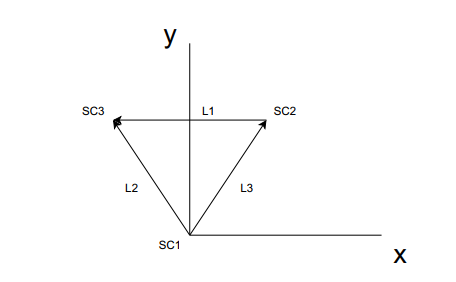
\includegraphics[width=12cm]{TianQin_config.png}
\caption{天琴探测器构型,参考文献\cite{zhang2020full}}
\label{fig2-LISA_con}
\end{center}
\end{figure}

%描述坐标系转换关系,得到臂长表达式或臂长变化量表达式。
由前人的工作\cite{hu2018fundamentals,ye2019optimizing}\cite{luo2016tianqin}\cite{tan2020impact}\cite{zhang2020full},%假如某一波源在黄道坐标系$h(\bar{\theta},\bar{\phi},\hat{\Omega})$可以得到天琴探测器在黄道坐标系(笛卡尔坐标表示)中的表示为:
天琴探测器轨道在探测器质心坐标系下表示如下所示。
\begin{equation}
x(t)=R\cos(\alpha)+\frac{1}{2} R \cdot \emph{e} \cdot \cos(2\alpha-3) +d(\cos(\theta) \cos(\phi)\cos(\gamma)-\sin(\phi)\sin(\gamma)) 
\end{equation}
\begin{equation}
\mathcal(y)(t)= R \sin (\alpha)+\frac{1}{2}R\cdot \emph{e} \cdot \sin (2\alpha)+d(\cos \theta \sin \phi \cos \gamma + \cos \phi \sin  \gamma)
\end{equation}
\begin{equation}
z(t)=-d \sin \theta \cos \gamma
\end{equation}
其中 $\alpha = 2\pi f_{\emph{e}} t+\mathcal{k}$是地球绕太阳的近日点角,$\mathcal{\Omega}$是初始角。
$\emph{e}$是地球离心率,并对其进行小量展开,保留到一阶。
$R$是地球轨道半长轴。
$d$是天琴探测器与地球之间的距离,目前设计为$10^8$米。

%需要说明坐标系转换关系: 从黄道坐标$(\bar{\theta},\bar{\phi})$,如何转换到探测器坐标下臂长的变化量。
在此基础上,探测器的臂长就能由其三角型的构型及其轨道来进行表示。参考时间记$t=0$
则臂长向量可表示为:
\begin{equation}
l_2^a=\cos{\frac{\gamma}{2}}x^a -\sin{\frac{\gamma}{2}y^a}
\end{equation}
\begin{equation}
l_3^a=\cos{\frac{\gamma}{2}}x^a +\sin{\frac{\gamma}{2}y^a}
\end{equation}
其中$\gamma=\frac{\pi}{3}$是SC1的顶角。



%说明迈克尔逊干涉原理
前面已知天琴可构造一对双臂长探测器,因此天琴能够同时探测引力波的两个偏振。基于文献\cite{cornish2001space}\cite{cornish2003lisa}\cite{cutler1998angular},引力波经过探测器会引起臂长变化。考虑波源是在黄道坐标$(\bar{\theta},\bar{\phi})$下,考虑引力波传播方向$\Omega$的自由度,引入极化角来组成新的正交坐标系$\left(
\hat{p},\hat{q},\hat{\psi} \right)$。
\begin{equation}
\hat{p}=\cos \psi\hat{\theta} +\sin{\psi}\hat{\phi}
\end{equation}
\begin{equation}
\hat{q}=-\sin\psi \hat{\theta} + \cos \psi \hat{\phi}
\end{equation}

%在x-y平面内,当$|\bf{x}-\bf{y}|$表示向量$\textbf{x}$和向量$\textbf{y}$笛卡尔距离,则构造单位向量:
%\begin{equation}
%\hat{r}_{ij}(t_i)=\frac{\textbf{x}_j(t_j)-\textbf{x}_i(t_i)}{L_{ij}(t_j)}
%\end{equation}
在静态近似(static limit)和低频近似(low frequency limit)的条件下
单个探测器响应函数可以表示为:

\begin{equation}
\begin{aligned}
h_I(t) &= \frac{\left [\delta L_1(t)-\delta L_2(t) \right ]} {L} \\ 
& =\frac{\sqrt{3}}{2}(\frac{1}{2}h_{xx}-\frac{1}{2}h_{yy}) \\
& =\frac{\sqrt{3}}{2}(A_{+}F^+_I(\theta_S,\phi_S,\psi_S)+A_{\times}F_I^{\times}(\theta_S,\phi_S,\psi_S))
\end{aligned}
\end{equation}

%说明低频近似的表达式
\begin{equation}
F^+_I(\theta_S,\phi_S,\psi_S)=\frac{1}{2}(1+\cos^2\theta_S)\cos 2\phi_S \cos 2\psi_S -\cos\theta_S \sin2\phi_S \sin 2\psi_S
\end{equation}
\begin{equation}
F_I^{\times}(\theta_S,\phi_S,\psi_S)\frac{1}{2}(1+\cos^2\theta_S)\cos 2\phi_S \sin 2\psi_S +\cos\theta_S \sin2\phi_S \cos 2\psi_S
\end{equation}

同理得到探测器"II"的响应后信号为
\begin{equation}
\begin{aligned}
h_{II} &= \frac{\sqrt{3}}{2} \frac{\left [\delta L_1(t) + \delta L_2(t) - 2 \delta L_3(t) \right]} {L}\\ 
& =\frac{\sqrt{3}}{2}(\frac{1}{2}h_{xy} +\frac{1}{2}h_{yx})
\end{aligned}
\end{equation}
且对探测器$II$的响应函数为:
\begin{equation}
F^+_{II}(\theta_S,\phi_S,\psi_S)=F_I^+(\theta_S,\phi_S-\frac{\pi}{4},\psi_S)
\end{equation}
\begin{equation}
F^{\times}_{II}(\theta_S,\phi_S,\psi_S)=F_{II}^{\times}(\theta_S,\phi_S-\frac{\pi}{4},\psi_S)
\end{equation}

由于引力波波长远远大于LISA探测臂长,故而每一组得到的迈克尔逊信号也可表示n阶谐波之和,故而可表示为$h_{\alpha}(t)\ =\ \sum_n \ h_{\alpha,n}(t) \ (\alpha=I,II),$。而其中$h_{\alpha,n}(t)$定义如(\ref{halpha})所示。故而这得到信号函数是($\theta ,\phi ,\varphi$)的函数,而这是三个自变量又随时间演化。对于不同空间探测器,主要体现在这三个角度的函数关系式不同,但是与引力波响应函数表达式是相同的。
%说明全天平均响应函数
%说明TDI*



\begin{comment}
由三角形几何关系可得
\begin{equation}
l\ =\ \frac{L_1 L_2 L_3}{\sqrt{2L_1^2 L_2^2 + 2L_2^2 L_3^2 + 2L_3^2 L_1^2 - L_1^4 -L_2^4 - L_3^4}}
\end{equation}


在激光干涉仪数据流中,数据是测量探测器两臂的激光在同一时间t内的相位差来构造,从而得到了三个航天器相关的TDI观测值。激光沿臂长$L_i$移动所需的时间$\tau_i = L_i/c$,其中$c$是光速。
由于航天器臂长是不相等的。则对应航天器1相关联的TDI响应信号是,
\begin{equation}
X(t)\ =\ s_1(t)\ -\  s_1(t-2\tau_2)\ -\ s_2(t)\ +\ s_2(t-2\tau_1) \label{eq2-tdi-1}
\end{equation}

其中$s_i(t)$是某个时刻到达航天器i的输入信号。则采用$1->2->3->1$顺序表示,其他相应两个航天器的响应信号如公式\ref{eq2-tdi-2}和\ref{eq2-tdi-3}所示。
\begin{equation}
Y(t)\ =\ s_2(t)\ -\  s_2(t-2\tau_3)\ -\ s_3(t)\ +\ s_3(t-2\tau_2) \label{eq2-tdi-2}
\end{equation}
\begin{equation}
Z(t)\ =\ s_3(t)\ -\  s_3(t-2\tau_1)\ -\ s_1(t)\ +\ s_1(t-2\tau_3)  \label{eq2-tdi-3}
\end{equation}

故而由方程(\ref{eq2-tdi-1}-\ref{eq2-tdi-3})可构造三个通道,即A、E、T 通道,到达扣除激光相位噪声的目标,且使得数据之间独立。各个通道表示如公式(\ref{eq2-A} - \ref{eg2-T})所示。
\begin{align}
A\ =\ \frac{1}{3}(2X\ -\ Y\ -\ Z)  \label{eq2-A} \\
E\ =\ -\frac{1}{\sqrt{3}}(Z\ -\ Y) \label{eq2-E} \\
T\ =\ -\frac{\sqrt{2}}{3}(X\ -\ Y\ -\ Z) \label{eq2-T}
\end{align}

A、E 和T通道数据是不相关的。且T通道在低频频段对引力波信号不敏感,只有A和E通道包含引力波信,可用于信号的搜索和分析。


实际上,采用TDI方法计算引力波相位变化对内存和计算力需求很高,故而目前空间探测器都是采用低频近似方法(Low frequency approximation)得到一对双臂探测器输出探测器信号(orthogonal signals)。令$l_1^i$,$l_2^i$,$l_3^i$作为沿着探测臂方向的单位矢量。取$L_i(t)$ 代表探测器第i个臂长。不同臂长可以组成不同探测器。三个臂长可组成两组迈克尔逊信号,且这两组信号相互垂直。如臂长1 和臂长2 可组成一组探测器I。 以LISA响应为例\cite{Cutler1998},则第一组探测器信号(即引力波强度)可以表示为:
\begin{equation}
h_I(t)\ =\ [\delta L_1(t)-\delta L_2(t)]/L = \frac{1}{2}h_{ij}(t)(l_1^il_1^j - l_2^il_2^j)=\frac{\sqrt{3}}{2}(\frac{1}{2}h_{xx}-\frac{1}{2}h_{xy}) \label{hI}
\end{equation}
第二组探测器信号则可表示为:
\begin{align}
  h_{II}(t) &=\  3^{-1/2}[\delta L_1(t) +\delta L_2(t) - 2\delta L_3(t)]/L        \\
             &=\  \frac{1}{2\sqrt{3}} h_{ij}(t)(l_1^il_1^j + l_2^il_2^j - 2l_3^il_3^j) =\frac{\sqrt{3}}{2}(\frac{1}{2}h_{xy}+\frac{1}{2}h_{yx}) \label{hII}
\end{align}
公式($\ref{hI}$)和($\ref{hII}$)中需要运用的坐标转换关系,其中$l_i^{\alpha}=cos\gamma_i x^a+sin\gamma_i y^a$,$\gamma_i=\pi/12+ (i-1)\pi/3$,$l_i^a$是沿探测臂的单位矢量,$x^a$和$y^a$分别是探测器坐标系下沿着x轴和y轴的单位矢量,$a=x,y,z$是三维空间指标。

由上一章可知,探测器响应函数跟引力波信号是线性关系,并且考虑空间探测器方位角$(\theta , \phi)$和偏振角$\varphi$,则响应后的引力波信号可表示为
\begin{equation}
h_{\alpha,n}(t)=\frac{1}{D}\frac{\sqrt{3}}{2} [ F^+_{\alpha}(t)A_n^{+}(t) + F^{\times}_{\alpha}(t)A_n^{\times}(t)] \label{halpha}
\end{equation}
%其中$A_n^{+,\times}$是由对EMRI 源进行特征表示的波形模型中的两种偏振模式系数。而系数$\frac{\sqrt{3}}{2}$是LISA臂长实际倾角是60°而不是90°。$F_{\alpha}^{+,\times}$是LISA探测器响应函数,具体表示如公式所示。
\begin{align}
 F_I{+}\      &=\  \frac{1}{2}(1+cos^2\theta)cos(2\phi)cos(2\varphi)-cos\theta sin(2\phi)sin(2\varphi)       \\
 F_I{\times}\ &=\  \frac{1}{2}(1+cos^2\theta)cos(2\phi)sin(2\varphi)+cos\theta sin(2\phi) cos(2\varphi)       \\
  F_{II}{+}\      &=\  \frac{1}{2}(1+cos^2\theta)sin(2\phi)cos(2\varphi)+cos\theta cos(2\phi)sin(2\varphi)       \\
 F_{II}{\times}\ &=\  \frac{1}{2}(1+cos^2\theta)sin(2\phi)sin(2\varphi)-cos\theta cos(2\phi) cos(2\varphi)
\end{align}


由于引力波波长远远大于LISA探测臂长,故而每一组得到的迈克尔逊信号也可表示n阶谐波之和,故而可表示为$h_{\alpha}(t)\ =\ \sum_n \ h_{\alpha,n}(t) \ (\alpha=I,II),$。而其中$h_{\alpha,n}(t)$定义如(\ref{halpha})所示。故而这得到信号函数是($\theta ,\phi ,\varphi$)的函数,而这是三个自变量又随时间演化。对于不同空间探测器,主要体现在这三个角度的函数关系式不同,但是与引力波响应函数表达式是相同的。

在考虑不旋转的探测器坐标系下,基于初始空间方位角$(\theta_S,\phi_S)$和初始相位角$\phi_0$,上述三个角度的演化公式如\ref{theta-t}所示。
\begin{equation}
cos \theta(t) = \frac{1}{2}cos \theta_S -\frac{\sqrt{3}}{2} sin \theta_S cos[\bar{\phi_0} + 2\pi(t/T) - \phi_S]
\label{theta-t}
\end{equation}
\begin{equation}
\phi(t) = \bar{a_0} + 2\pi(t/T) + tan^{-1}[\frac{\sqrt{3}cos \theta_S + sin \theta_S cos[\bar{\phi_0} + 2 \pi(t/T) - \phi_S]}{2 sin \theta_S sin[\bar{\phi_0}+ 2\pi(t/T)-\phi_S]}
\end{equation}
\begin{equation}
tan \psi =\frac{A} {B}
\end{equation}
其中
\begin{equation}
A= \{ \frac{1}{2} cos \theta_L - \frac{\sqrt{3}}{2} sin \theta_L cos[\bar{\phi_0} + 2\pi (t/T)-\phi_L] - cos \theta(t) [cos \theta_L cos \theta_S + sin \theta_L sin \theta_S cos(\phi_L - \phi_S]  \}
\end{equation}



\begin{equation}
\begin{split}
B=&[\frac{1}{2}sin \theta_L sin \theta_S sin(\phi_L - \phi_S) - \frac{\sqrt{3}}{2}cos(\bar{\phi_0} + 2\pi (t/T)) (cos \theta_L sin \theta_S sin \phi_S - cos \theta_S sin \theta_L sin \phi_L ) \\
&- \frac{\sqrt{3}}{2}sin (\bar{\phi_0} + 2 \pi (t/T)) (cos \theta_S sin \theta_L cos \phi_L - cos \theta_L sin \theta_S cos \phi_S)]
\end{split}
\end{equation}


%\begin{figure}[htbp]
%\begin{center}
%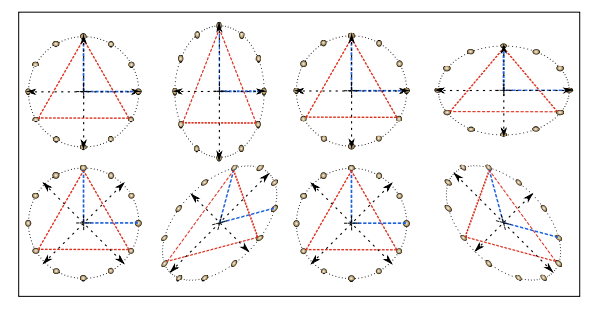
\includegraphics[width=12cm]{Figures/Chapter02/LISA.PNG}
%\caption{引力波经过LISA探测器平面引起的变化;图片来自\cite{Mitryk2012}}
%\label{fig1.1}
%\end{center}
%\end{figure}

\end{comment}



%\section{天琴对EMRI的探测能力}
范会敏等人\cite{Fan:2020zhy}基于理想信噪比的计算和FIM(Fisher Information Matrix)的方法评估了天琴对EMRI这类波源的探测事件率和物理参数估计精度。%
%事件率计算和结果。
%参数估计计算和结果

\chapter{EMRI信号探测}
%第二章介绍信号处理基础,二元统计假设检验理论,探测算法,参数估计算法。
%cite{7Ryan1995}~\cite{8Ryan1997}。

在混杂高斯噪声的引力波信号中,这需要一些工具去满足理论研究的需要和实际计算。这里面就包括了理想信噪比的计算,Fisher矩阵、误报率和探测率、$\mathcal{F}$-统计量($\mathcal{F}$-statisic)和
模板(Template placement)以及拟合因子(Fitting Factor)\cite{jaranowski2012gravitational}\cite{cutler1994gravitational}。

本章介绍数字信号处理基础,信号探测原理,通过介绍部分二元统计假设检验理论,解释探测算法原理,给出现有EMRI信号探测算法,和参数估计算法。

\section{波形模板及波形模板库}
在EMRI信号探测任务中,基于模板的算法都需要建立一个模板库,比如半相干搜索算法、MHMC算法等等。其他不基于模板的算法也需要产生模拟信号,比如time-frequency算法(Time-frequency method)。基于EMRI信号的产生机制和不同波形波形,我们产生不同数量的EMRI信号。下面提供采用AK波形模型和AAK波形模型来产生EMRI信号的源参数取值范围。

%模板数的计算
为了评估在持续时间$T$的一致性搜索所需要的模板数,一般会在模板空间上建立一个度规来进行描述(也即在参数空间上建立度规)\cite{owen1996search,balasubramanian1996erratum}。


%模板定义
在双星系统中,波形模板一般用$h(t,\mu,\lambda)$来描述,在波形的参考时刻$t$, ``$\mu$"是波形的外禀参数,``$\lambda$"是波形的内禀参数。$\lambda^i$内禀参数比如双星的质量和自旋,$\mu^i$比如双星最后的并合时刻$t_0$和并合相位$\Phi_0$。模板库一般会被归一化,即\cite{owen1996search}
\begin{equation}
\langle h(\mu,\lambda) |  h(\mu,\lambda) \rangle = 1
\end{equation}
对所有$\mu$和$\lambda$取值成立。

%定义参数空间度规
参数空间的度规建立,需要结合拟合因子(Fitting Factor)和匹配滤波的结果来考虑,综合信噪比和事件率的损失来建立参数度规。
一般而言,假如探测器输出信号能够与模板匹配,则能够得到理想信噪比。对于固定的内禀参数而言,外禀参数(影响振幅值)可以更快通过归一化计算得到,故而参数空间的大小更加受内禀参数的影响,即搜索一个信号在有效的模板空间应该满足
\begin{equation}
\mathop{\rm max}\limits_{k}   \left [ \mathop{\rm max}\limits_{\mu} \langle \ d | h(\mu,\lambda) \rangle \right ]
\end{equation}
故而针对模板库中两个模板的匹配系数(match)如下定义,这也是假设检验中的模糊函数的定义(ambiguity function)\cite{owen1996search}
\begin{equation}
\rm M(\lambda, \Delta \lambda) \equiv  \mathop{\rm max}\limits_{\mu,\Delta \mu} \langle \ h(\mu,\lambda)  | h(\mu +\Delta \mu ,\lambda+\Delta \lambda) \rangle 
\label{eq:match}
\end{equation}
使用公式\ref{eq:match}来描述两个波形的相似性。当匹配系数取得最大值时,$\Delta \lambda =0$,同时将公式多阶展开,得到的表达式如下:
\begin{equation}
\rm M(\lambda, \Delta \lambda) \approx 1 \ + \ \frac{1}{2} \left( \frac{\partial^2 \rm M }{\partial \Delta \lambda^i \partial \Delta \lambda^j} \right)_{\Delta \lambda^k=0}\Delta \lambda^i \Delta \lambda^j
\end{equation}
由此可以在参数空间上建议一个度规
\begin{equation}
g_{ij}(\lambda) =-  \ \frac{1}{2} \left( \frac{\partial^2 \rm M }{\partial \Delta \lambda^i \partial \Delta \lambda^j} \right)_{\Delta \lambda^k=0}
\end{equation}
所以不匹配系数的计算也可以定义为两个模板之间的距离。
\begin{equation}
1-\rm M = g_{ij}\Delta \lambda^i \Delta \lambda^j
\end{equation}

%求出最小匹配的值mimimal match
建立内禀参数空间(N-维)的度规之后,假设该参数空间步长为$dl$。假如一个信号存在空间中的某个格点上,最小的信噪比应该满足$E(\rho)$。而那些足够相近的模板,$\emph{i.e.} \ dl \ll 1 $,在这样的参数空间满足公式
\begin{equation}
g_{ij}\Delta \lambda^i \Delta \lambda^j= N(dl/2)^2
\end{equation}
考虑事件率损失和最小信噪比,定义了最小的匹配系数
\begin{equation}
\rm MM = 1 - N(dl/2)^2
\end{equation}
通过计算最小匹配系数得到一个最小的参数空间格点,将参数空间划分按照最小格点划分的格子数就是一个模板所需要要的模板数。
\begin{equation}
\mathcal{N} = \frac{\sum d^N \lambda \sqrt{det||g_{ij}||}}{\left[ 2\sqrt{(1-\rm MM)/N} \right]^N}
\end{equation}
假定最小匹配系数$\rm MM=0.97$,实际计算需要考虑双星系统的内禀参数和参数的最小步长,由于探测器的灵敏度会影响最小步长的设计,所以提升探测器的灵敏度能减少模板数。

%得到EMRI如何评估所需要的模板数


%得到EMRI如何评估所需要的模板数



\begin{comment}
\section{数字信号处理基础}

%首先介绍数字信号处理的一些概念,
由Nyquist采样定理可知,保证信号不失真条件下,采用频率至少是在限带宽信号中最大频率的两倍$f_{max}$。信号与噪声的统计特性是不同,先介绍噪声的统计特性,再介绍与信号相关内容。

%\subsection{噪声的统计特性}
%\subsection{Fisher矩阵}
%\subsection{拟合因子}
在探测器中,仪器噪声可近似为一个随机过程,故尽管我们不知仪器噪声的实际时间序列$x(t)$,我们也可用随机过程的统计特性描述噪声的特性。
如果该随机过程的统计特性不随时间改变统计特性,则称为平稳随机过程。则该总体均值也等价于总时间上的均值,所以$x$的期望值也可写为:
\begin{equation}
\left \langle x \right \rangle :=\  \lim\limits_{T \to \infty }{\frac{1}{2T}\int^{T}_{-T}x(t)dt}.
\end{equation}

在这样的平稳随机过程中,常见的一类就是高斯过程(Gaussian process),可以由其期望值和功率谱密度函数来描述。


{\bfseries{ 功率谱密度函数(Power Spectrum)}}

取该某个随机过程是均值为0 的分布,即\ $\left \langle x \right \rangle =\ 0$\ 。则功率可以定义为在\ $T$\ 时间内\ $x^2(t)$\ 除以 \ $T$\ 。如果该过程是平稳的,则若\ $T$\ 足够的大,则\ $x^2(t)$\ 的时间均值就等价于\ $x^2(t)$\ 的期望值,即\ $\left \langle x^2(t) \right \rangle = 0$ 。
\begin{equation}
%\left \langle x^2(t) \right \rangle :=\  \lim\limits_{T \to \infty }{\frac{1}{2T}\int^{\infty}_{-\infty}x^2(t)dt}.
\left \langle x^2(t) \right \rangle :=\  \lim\limits_{T \to \infty }{\frac{1}{2T}\int^{T}_{-T}x^2(t)dt}.
\end{equation}

由{\bfseries{Parseval}}定理可知:信号能量守恒,${\int^{\infty}_{-\infty}x^2(t)dt}\ =\ {\int^{\infty}_{-\infty}|x(f)|^2df}$\ ,由$\ref{td}$\ 得到$\ref{fd}$\ ; 且傅里叶变换是关于实数域的偶函数,即$\tilde{x}(-f)=\tilde{x}^*(f)$\ ,因而由$\ref{fd}$\  得到$\ref{ft}$\ ;由功率谱函数的定义:
\begin{equation}
\     \  S_x(\omega)\  :=\  \lim\limits_{T \to \infty }{\frac{1}{2 \pi T}|\tilde{x}(\omega)|^2}.
\end{equation}
\ $\  \tilde{}\   $\ 代表傅里叶变换,$\tilde{x}\ =\ \int^{T}_{0} dt\ x(t)e^{-j\omega t} $,由傅里叶变换的性质,也可得:$S_x(-\omega) = S_x{(\omega)}$
则由$\ref{ft}$\  得到$\ref{sw}$\

即:
\begin{align}
  \left \langle x^2 \right \rangle &=\  \lim\limits_{T \to \infty }{\frac{1}{2T}\int^{T}_{-T}x^2(t)dt}\label{td}        \\
             &=\  \lim\limits_{T \to \infty }{\frac{1}{2T}\int^{T}_{-T}|\tilde{x}(f)|^2df}\label{fd} \\
             &=\  \lim\limits_{T \to \infty }{\frac{1}{T}\int^{T}_{0}|\tilde{x}(f)|^2df} \label{ft} \\
             &=\   {\int^{\infty}_{0}S_x(f)}df  \label{sw}
\end{align}

$|x(f)|^2df$频率在$f$ 和 $f+df$内$x(t)$的分量对总能量的贡献。$\tilde{x}(f)^2$ 表示某频率$f$处的能量密度。

~\\
{\bfseries{ 自相关函数(Autocorrelation Function)}}

自相关函数的定义是:$R_x(\tau)\  :=\  \left \langle x(t)x(t+\tau )  \right \rangle$。
由$\bf{Wiener-Khinchin}$ 定理知,功率谱密度函数是自相关函数的的傅里叶变换,即
\begin{align}
\    &S_x(\omega) = \int^{\infty}_{-\infty} R_x(\tau) e^{-j\omega t} d\tau \\
\    &R_x(\tau) = \frac{1}{2 \pi}\int^{\infty}_{-\infty} S_x(\omega) e^{j\omega \tau} d\omega
\end{align}

自相关函数反映信号的周期性,功率谱密度反映信号在各个频率上的能量。白噪声是在整个频谱上能量不变的信号,即一条平行于X轴的直线,更具傅里叶变换的性质,其傅里叶反变换(信号的自相关函数)是狄拉克函数,即冲击函数。
\end{comment}

\section{信号检测理论}
如何从得到数据中得到引力波信号?这是本章要讨论的问题。通过观测数据判断信号是否存在,这一问题称为信号检测,本质上是一种统计假设检验。从计算角度看,信号检测理论(Signal Detection Theory)是一种计算框架(computational framework ),它描述如何从噪声中抽取信号,同时对可能影响抽取过程的偏差和其他因素做出解释。

所谓“统计推断”,是指对随机变量的统计特性(如概率分布等)的有关假设作出推断。本质上,假设是关于感兴趣的一个主体的某个未知特征的主张,常用H 表示统计假设。例如,关于引力波目标信号的存在,可以提出下列的假设:

$H_0$ : 目标信号不存在 $\ s(t)\ =\ n(t)$

$H_1$  : 目标信号存在\  $\ s(t)\ =\ n(t)\ +\ h(t)$\\
其中$\ s\ $代表数据,$\ n\ $代表噪声,$\ h\ $代表引力波信号,他们都是关于时间$t$的函数。{\bfseries{目标信号}}就是我们感兴趣的{\bfseries{主体}},而{\bfseries{存在}}就是这些总体的{\bfseries{未知特征}}。

只有两个统计假设$\ H_0\ $ ?和$\ H_1\ $的问题称为二元统计假设检验问题。%习惯使用$\ H_0\ $ 表示随机事件不发生的基本假设, $\ H_1\ $表示随机事件偶然发生的假设。基本假设$\ H_0\ $ 称为零假设(null hypothesis)或原(始)假设(original hypothesis),与之对立的假设$\ H_1\ $称为备择假设(alternative hypothesis)或对立假设。
因此这个二元统计假设检验的基本问题是:对假设$H_0$是否为真做出具体判断。为此,需要设计一种规则,它能够根据实验数据对是否拒绝$H_0$ 假设做出判断。这种规则称为统计假设检验。关于一个统计假设的决策本质上是基于观测数据的统计量的一个推断过程。




而当要从已知噪声统计特性过程中抽取信号,这种可以构造理想探测统计量。理想统计量最能简单直接量化表明数据中含有期望信号的概率。继续采用以上的假设可知,可采用似然比值$ O(H_1|s)\ =\ P(H_1|s)\ :\ P(H_0|s)$。这个比值的含义是:在给定数据$s(t)$的情形下,备选假设$\ H_1\ $是成立的概率与零假设$\ H_0\ $成立的概率。而计算这个比值会有多种种方法,比如:Neyman-Pearson准则、一致最大功效准则、贝叶斯准则。%而采用贝叶斯准则也是后面匹配滤波算法作为探测信号的原理。$\\ $

%统计判决准则
理论上信号是否存在的条件概率分布式不一样的,因而信号能够被正确检测。实际上,由于数据有观测噪声且数据是有限长的等因素的存在,决策统计量(似然函数比)的估计就不免出现误差,出现信号数据被检测为噪声,噪声数据被检测为信号。即在二元假设检验问题上,会存在两类错误。在第一类错误中,$H_0$假设为真却被拒绝,其发生概率也被称为误报率(False Alarm Probability),体现的是检测显著性(significance of the test)。在第二类错误中,$H_1$假设为真但判决为$H_0$为真,其发生概率也被称为漏警率(Dismisal Probability),体现的是检测能力(Power of the test)。
则第一类错误概率定义为$H_0$假设下决策统计量$g=g(y)$大于阈值Th 的条件概率$P(g>Th|H_0$)。
% 画出决策空间图像

%统计量的阈值确定
一般而言,探测统计量的阈值是由误报率决定的。
\begin{equation}
\rm Th = \frac{\sqrt{2}\sigma}{\sqrt{N}} \rm erfc^{-1} (2\alpha)
\label{eq:threshold}
\end{equation}
其中``Th''是阈值,``$\sigma$''是噪声的方差,``$N$''是数据样本长度,``$\alpha$''是误报率。

%{\bfseries{ 贝叶斯理论(Bayes's Theorem)}}


%由条件概率的定义可得$\ P(A|B):=\frac{P(A,B)}{P(B)}\ $ 且$\ P(B|A):=\frac{P(A,B)}{P(A)}\ $,故而联立两个方程可得,$P(B|A):=\frac{P(B)P(A|B)}{P(A)}$
%在方程中,$P(B)$是先验概率函数,$P(A)$是A的边缘分布概率函数,也是证据量(evidence),在方程中视为一个归一化常数。$P(B|A)$是在A成立的条件下B 成立的后验概率,$P(A|B)$ 是假定B成立条件下A成立的概率函数。

%贝叶斯理论提供了一个完备的关系:$P(A)\ =\ P(A|B)P(B)+P(A|\neg B)P(\neg B)\ $,其中$P(\neg B)=1-P(B)$。由此,我们可以发现,
%\begin{equation}
%P(B|A)=\frac{P(B)P(A|B)}{P(A|B)P(B)+P(A|\neg B)P(\neg B)}=\frac{\Lambda (B|A)}{\Lambda (B|A)+P(\neg B)/P(B)}
%\end{equation}
%其中$\Lambda (B|A):=\frac{P(A|B)}{P(A|\neg B)}$ ,这是一个似然比。
在引力波探测中,一般采用Neyman-Pearson 准则。
引力波信号微弱,所以更希望误报率高一点,也不允许错过一个引力波信号。这具体测度描述在后面探测测度中会描述。主要第二类错误不能发生太高,把有信号的数据当做没有信号而错过。

其后验概率分布中会出现很多局部最大值,这是由EMRI信号本身的特点所决定的。一个EMRI信号是由三个基本轨道相关频率所组成的多阶谐波构成,这三个频率分别是,且他们都随着时间变化而演化。这些谐波不同于强度(strain),也不同于由于不同时间匹配最强引力波相位谐波带来的局部最大值。
%It is possible for a signal with very different parameters to match the dominant harmonic very well for the whole duration of the signal but miss completely all the other harmonics.
%Babak \cite{Babak2009}他们组的看法是


该类任务可以看作引力波天文学、信号处理(随机信号)和信息通信、统计学交叉的领域。所以从随机信号的角度来解读信息是基础。
\begin{comment}
在信息论和统计学中,信息熵简称为熵,是表示随机变量的不确定性的度量。信息熵是对信息的量化度量,它对于通信、数据压缩等等都有很强的指导意义。

假设数据D是一离散型随机变量,其概率分布为:
$$P(D=d_k)=p_k,\  k=1,2,3,...,n$$
则随机变量的信息熵定义为:
$$H(D)=-\sum^n_{i=1} p_i \ \times  \ log p_i,\ i =1,2,3,...,n$$
$log p_i$ 是以2为底的对数。
\end{comment}

\section{传统探测算法}
%探测的各个方法可以各自写一节
%自己采用的算法实验及结果写一节
从是否采用模板匹配提取信号的角度,传统探测算法可以分为匹配模板类算法和非匹配模板类算法。匹配模板类算法包括半相干算法、$\mathcal{F}$-统计等方法。非匹配类模板主要是时间-频率算法。 本节主要介绍这些两大类算法特性、适用场景和优缺点。

\subsection{匹配模板类算法}
%Matching Filtering
由前面内容讨论可知,对于“探测”问题,我们期望能通过似然比的计算,从而得到探测信号的概率比值。即表示如下,
\begin{equation}
\Lambda (H_1|s)= \frac{p(s|H_1)}{p(s|H_0}
\end{equation}
(在实际计算中,采用概率密度函数代替概率函数。)

假设噪声是高斯噪声,则可计算概率密度函数在$H_0,s(t)=n(t)$假设下,$p(s|H_0) =P_n[s(t)]\propto e^{-(s,s)/2}$
%\begin{equation}
%\end{equation}
而在备选假设$H_1,n(t)=s(t)-h(t)$条件下,$p(s|H_1) =P_n[s(t)-h(t)]\propto e^{-(s-h,s-h)/2}$
%\begin{equation}
%\end{equation}
因此似然比作为探测统计量可以表示为
\begin{equation}
\Lambda (H_1|s)=\frac{e^{-(s-h|s-h)/2}}{e^{-(s,s)/2}}=e^{(s,h)}e^{-(h|h)/2}
\end{equation}
可以看到,似然比依赖于数据$s(t)$只通过内积$(s,h)$,更进一步说,内积的定义是,
\begin{equation}
(s,h):=4Re\ \int^{\infty}_0 \ \frac{\tilde{s(f)}\tilde{ h}^{\ast}(f)}{S_n(f)}
\end{equation}

由此也可知,信噪比也可以一个理想探测统计量。对于信噪比任何选定的阈值,其都能表示从噪声中多大概率认定为有信号的表征。因此$(s,h)$被称为匹配滤波。而h为给定的模板。



总的来说,匹配滤波是将探测器的输出乘以一个代表理想波形的模板函数(关于时间的函数),求和之后就是匹配滤波的结果。如果是纯粹的噪声,则乘积后的结果应当是很小的,自然达不到认定为信号的阈值。当然会存在误判的情形。关于阈值的选定,根据定义\ref{eq:threshold}同样在加性高斯白噪声($\mu=0,\sigma=1$)情况下,由于误报率与/或漏警率的不同,需要确定的阈值Th与/或样本长度N。假如误报率$\alpha=0.01$且$N=1000$(数据数目),则计算阈值为:
\begin{equation}
\rm Th=\frac{\sqrt{2}\sigma}{N}\rm erfc^{-1}(2\alpha)=\sqrt{2/N} \times 1.64 =0.0733
\end{equation}
%采用匹配滤波算法来探测引力波信号,前提是有匹配模板。


设定误报率$\alpha=0.1$,漏警率$\beta=0.05$,为了满足这些错误概率所需要设置的阈值$Th$和样本数目$N$
\begin{equation}
\alpha = \frac{1}{2} \rm erfc(\frac{\rm Th}{\sqrt{2/N}})
\end{equation}
\begin{equation}
\beta = 1-\frac{1}{2} \rm erfc \left (  \frac{\rm Th-1}{\sqrt{(2/N)}} \right )
\end{equation}
结合条件得到下面的方程。
\begin{comment}
\begin{equation}
Th = \frac{\sqrt{2}}{\sqrt{N}} \erfc^{-1}(2\alpha)=\frac{\sqrt{2}}{\sqrt{N}} \erfc^{-1}(0.2)
\end{equation}

\begin{equation}
\rm Th-1 = \frac{\sqrt{2}}{\sqrt{N}} \erfc^{-1}[2(1-\beta)]=\frac{\sqrt{2}}{\sqrt{N}} \erfc^{-1}(1.998)
\end{equation}
\end{comment}
两个方程得到的结果是
\begin{equation}
\frac{Th}{Th-1}=\frac{erfc^{-1}(0.2)}{erfc^{-1}(1.998)} =\frac{0.91}{-1.16} =-0.784
\end{equation}
解得$Th=0.439$.将这个阈值带入$Th=\frac{\sqrt{2}}{\sqrt{N}} erfc^{-1}(0.2)=\frac{\sqrt{2}}{\sqrt{N}} \times 0.91 =0.439$,故而$N=9(8.593)$





\subsubsection*{半相干算法}
在Cutlter等人首次估计EMRI事件率的时候,采用半相干算法进行了探测EMRI事件。而半相干算法是在Pletsch等人\cite{pletsch2010parameter}引入到进行连续引力波信号探测。

%算法的核心思想和过程
由于一个EMRI信号用14个物理参数进行波形建模,计算所需的模板数达$10^{40}$个。无论考虑多少计算效率的提升,采用一个全数据直接匹配模板的方法,穷尽计算资源也不能完成计算。故而采用了半相干算法。将整个观测数据分成多个子段。对每个子段的探测统计量求和,即该统计量之和近似于真实观测数据的探测统计量值。

%展开说明细节
假如一个四极引力波可以解析为5阶谐波$h_i(\lambda_\alpha;t)$(i=1,2,...,5), 内禀参数主要影响波形相位,外禀参数主要影响波形振幅。当一个数据分为$N$段,每段探测统计量为信噪比的平方。
\begin{equation}
\rho^2 = \sum_{\alpha=I}^{II} \sum_{i=1}^{5} \langle h_i(\lambda_\alpha),S_\alpha \rangle^2
\end{equation}
其中``<>''是$\langle a,b \rangle = 4\mathcal{R} \left [\frac{\tilde{a}^{\star}(f)\tilde{b}(f)}{S_b(f)} df  \right ]$
$S_b(f)$是$b$探测器的单边功率谱密度。 $\tilde{\alpha}$是$\alpha$的傅里叶变换后的数据。在$\rho^2$中是将外禀参数最大化。

算子段(single-segment)探测统计量时,采用的模板参数空间可以称为``粗网格"(coarse grid),记参数空间的某一个格对应的参数集为$\hat{\lambda}$;而对应单个全数据来说,采用的模板参数空间可以称为``细网格"(fine grid)。前者把参数空间划分的格数是小于或等于后者的格数。



%算法的适用场景和优劣势。


\subsubsection*{$\mathcal{F}$-统计}


% 介绍算法的核心思想
%为了搜索到引力波信号,使用$\mathcal{F}$-统计方法只需要在内禀参数空间上进行。
%由于假设仪器噪声是高斯平稳的高斯过程,则统计量$\mathcal{F}$符合

将所有物理源参数空间化作网格,每个网格格点意味着一个模板。当引力波波源参数越多,则源参数的联合概率分布越复杂,参数空间也越高维。在探测信号过程,越高效地计算探测统计量就变得越重要。从传统意义上说,似然函数比通常作为探测统计量。
%说明因由
\cite{jaranowski1998data, prix2007statistic}在搜索连续引力波时使用$\mathcal{F}$-统计的方法来计算似然函数比。这也是基于模板匹配的算法。一个数据的似然函数比通常表示为公式\ref{eq:likelihood_ratio}。
\begin{equation}
log \Lambda (\bf{\theta}) = (s|h(\bf{\theta}))-\frac{1}{2}(h(\bf{\theta}|h\bf{\theta})
\label{eq:likelihood_ratio}
\end{equation}
其中h为单个波形模板,$s$为数据。要得到最优的参数集合$\theta$,取$L(\bf{\theta})=log\Lambda(\bf{\theta})=\langle{s|h(\theta)}\rangle - \frac{1}{2}\langle h(\theta)|h(\theta) \rangle$,令$\frac{L(\theta)}{\partial \theta}=0$ 则我们就能在参数空间上取得极值。

在王龑\cite{wang2012extreme}对EMRI波形采用的是唯象波形(PW)。在源坐标下,一个单一谐波可以采用高阶相位(展开到2阶)来描述,则波形描述为如下形式。
\begin{equation}
h(t)=A_+ cos(\Phi(t)+\Phi_0)e_+ +A_{\times} sin(\Phi(t)+\Phi_0)e_{\times}
\end{equation}
\begin{equation}
\Phi(t)=2\pi f(t-t_0)+\pi \dot{f}(t-t_0)^2 +\frac{1}{3} f(t-t_0)^3 + \frac{\pi}{12}f(t-t_0)^4
\end{equation}
那么将这样一个源波形考虑上探测器的响应,则可以将波形分解成是否包含时间的两项。表示为两个响应后的信号
\begin{equation}
h_I(t)=A^{\mu}h_{\mu}^I(t),h_{II}(t)=A^{\mu}h_{\mu}^{II}(t)
\label{eq:simplified_wav}
\end{equation}
其中$A^{\mu}$是不含时间的变量,即不随时间发生演变,只取决于$A_+,A_{\times},\Phi_0,\Psi$, 这些是外禀参数,相对应的是$\mu=1,2,3,4$。然而$h_{\mu}^I,h_{\mu}^{II}$是($\theta^S,\phi^S,f,\dot{f}$)的函数,这些内禀参数会随时间发生变化。故而采用$\mathcal{F}$-统计方法来降维参数空间时,会将外禀参数约化为固定的常数,只对内并参数进行最大似然估计。
在实际数据中,将波形叠加了噪声后,得到的联合对数似然函数是每一个对数似然函数之和。
\begin{equation}
L(\theta,A^{mu}) =\langle S_i|h_i(\theta) \rangle -\frac{1}{2}\langle h_i(\theta) | h_i(\theta)\rangle
\label{eq:likelihood_ratio_data}
\end{equation}
这里$i=I,II$是两个正交引力波信号的指标。将方程\ref{eq:simplified_wav}带入方程\ref{eq:likelihood_ratio_data}中,得到似然函数为:
\begin{equation}
L(\theta,A^{\mu})=A^{\mu}s_{\mu}^{i}(\theta)-\frac{1}{2}A^{\mu} M^i_{\mu\nu }(\theta)A^\nu
\label{eq:MLE_1}
\end{equation}
其中$i=I,II$,
$S_\mu^i=\langle s_i |h_\mu^i\rangle$,
$M^i_{\mu\nu}=\langle h_\mu^i |h_\nu ^I \rangle$。将公式\ref{eq:MLE_1}中外禀参数约去,联合概率分布取导得到似然函数的极值,则得到方程。
\begin{equation}
\frac{\partial(L(\theta,A^mu)}{\partial A^\mu}=(s^I_{\mu}+ s^{II}_{\mu}) + (M^I_{\mu\nu}+M^{II}_{mu\nu})A^\nu =0
\end{equation}
则自然可以直接得到$A^\mu=[(M^I+M^{II})^{-1}]^{\mu\nu} \times (s^I_\nu +s^{II}_\nu)$。在外禀参数空间上将似然函数最大化,这就是$\mathcal{F}$-统计,可记为:
\begin{equation}
F(\theta) \equiv max L(\theta,A^\mu)=\frac{1}{2}(s^I_{\mu}+ s^{II}_{\mu})[(M^I+M^{II})^{-1}]^{\mu\nu} \times (s^I_\nu +s^{II}_\nu)
\end{equation}
则该$\mathcal{F}$值与信噪比联系起来得到如下公式。
\begin{equation}
E[F(\theta)] = \frac{1}{2} SNR^2 +2
\end{equation}

\begin{comment}
在模板库中任意取一个模板去计算似然函数比,则可化为矩阵形式。
\begin{equation}
log \Lambda = a^T N -\frac{1}{2}a^T M a
\end{equation}
其中$s$表示的是科学数据,且$s(t)=n(t)+h(t)$。向量$N$和矩阵$M$表示为
$$N^{(k)}:=(s|h^{(k)}),M^{(k)(l)}:=(h^{(k)}|h^{(l)})$$
对于采用最大似然估计方法(Maximum likehood estimation),外禀参数可以用最大似然估计得到$\hat{a}=M^{-1}N$
\end{comment}


%举例来说,计算双星并合产生的引力波得到的$\mathcal{F}$


\subsection{非匹配模板类算法}
不基于波形模板匹配的算法主要是时间-频率算法。基本思想是:将数据流按某一时长分割成段,再各自做傅里叶变换,可得到时间-频率-功率三维数据;再将其与相对应的噪声功率的统计分布做比较。如果是信号,他将不符合噪声功率的统计分布特性。如果是高斯稳态噪声,其概率分布函数符合$χ^2$分布;如果是非高斯平稳噪声,做白化操作后,可得到高斯噪声。
目前时间-频率算法可以分为超功率法和HACR法 。
	超功率法(Excess Power search method)\cite{gair2005detecting}
将数据流按照一段时间间隔分割,并做快速傅里叶变换。按照一定的时间间隔和一定的频率分割得到分段数据的功率,而频率是时间的函数,将选定时间与频率内数据中存在的功率,与已知的噪声功率的统计分布进行比较,如果探测器噪声是平稳高斯噪声,那么噪声功率将遵循 ${\chi}^2 $ 分布,其自由度数量等于时间-频率值的两倍。因此,设定引力波信号的误报率,调整持续观测时间和频带宽,可得到间隔$(bin step )$ 的大小
,
设定探测到引力波的阈值,如果超过该阈值,则该功率点值是信号功率点值。所以探测率的效率取决于持续观测时间、频率带宽,间隔大小,误报率设定值。Gair等人\cite{gair2005detecting}给出综合效益最好的探测结果是,在误报率为0.1\%的情况下,探测到2Gpc的经典EMRI信号(大质量黑洞质量为 $10^6 M_{\odot}$ 小天体的质量为$10M_{\odot}$)的探测率是$60\%$。但是该算法对盲数据(Blind Data,即未知源参数)的搜索效果却很差
	HACR法(Hierarchical Algorithm for Clusters and Ridges)\cite{gair2008constrained}
跟超功率法的基本思路一致,但是在搜索段功率值是否超过功率阈值时,会

探测器得到时域信号后,采用时间-频率分析法也是一种分层方法。第一层,将时间和频率进行分解,把已经记录到数据文件中的各个数据元[一段时间的信号]进行傅里叶变换,多数取3-4 个月数据。具体就是在固定的时间间隔内把探测到的数据抽样,对这
些数据切片进行傅里叶展开。把给定的频率间隔内存在的功率与已知的噪声功率的统计分布进行比较,寻找引力波存在的证据。在这种分析中,给定的频率间隔是时间的函数。对于不同源的处理方法不同,但手段很多,如对未知源,一般采用小波变换。

时间-频率分析方法是一种不依赖模板的方法。


\section{神经网络算法}

在当代计算机软硬件及网络的普及下,计算机的计算、存储和搜索能力显著提升,又因为大数据,由此打开了机器学习(Machine Learning, ML)、深度学习(Deep Learning, DL)\cite{Goodfellow_2016_MITpress} 的新格局。另一方面,近年来多信使天文学(Multi-Messenger Astrophysics,MMA)催生的科学需求,交叉领域的科学社区、科学平台及观测站都将慢慢发展起来,比如建立目标与观测管理系统(Target and Observation Manager System, TOM)、新一代望远镜(以更高精度定位引力波波源)等等[2018arxiv]。


本章介绍机器学习算法常用的目标函数(损失函数)、人工神经元的学习机制,依赖于反向传播算法来实现权重优化,从而更好地学习数据特征,区分数据集。接着介绍卷积神经网络及其基本结构,过渡到循环递归神经网络,用以处理引力波数据。

\subsection{目标函数和优化函数}

机器学习和深度学习\cite{Goodfellow_2016_MITpress, zhou2016machine, huang2017deep}是由数据驱动的科学。在分类问题上,他们的目的归结为尽量准确的学习到数据间的变量关系,还原样本数据的概率分布。如本文中,在已知数据条件下,求该数据是引力波信号的概率分布。交叉熵和相对熵正是衡量概率分布或者函数之间相似性的度量方法。
设有随机变量X,其真实概率分布是p(x),通过模型训练得到的概率分布为q(x),对于衡量q(x)和p(x)的相似性,我们可以用交叉熵和相对熵来衡量。

相对熵,全称是Kullback-Leibler Divergence, 也称为KL散度,KL距离,其定义为:
$$KL(p(x)||q(x)=\sum_{x \in X} p(x) \times log_2{(\frac{p(x)}{q(x)})} $$

相对熵不是传统意义上的“距离”,这是因为相对熵不具有对称性。当预测的分布q(x)与真实概率分布p(x)完全相同时,相对熵KL(p(x)||q(x))=0。如果两个分布的差异越大,那么相对熵越大;反之,两个分布的差异越小,那么相对熵越小。相对熵满足非负性,即$KL(p(x)||q(x))>=0$。相对熵最早用在信号处理上。

交叉熵全称为cross-entropy, 定义如\ref{eq:cross-entropy}示。
\begin{equation}
\label{eq:cross-entropy}
    H(p(x),q(x))=H(X) +KL(p(x)||q(x))
\end{equation}
其中H(X)表示随机变量X的信息熵,$H(X)=-\sum_{x \in X}p(x) \times log_2 p(x)$。由于真实分布p(x)是一个固定值,因此H(X)是一个不变量,故有:
$$H(p(x),q(x)) \approx KL(p(x)||q(x))$$
在深度学习领域,交叉熵代价函数(cost function)是常用的目标函数。

%\subsubsection{目标函数和优化算法}
针对信号探测问题,我们由探测原理可知,这是一个二元假设统计理论,对应到机器学习领域,这是一个分类问题。我们希望神经网络输出的结果也是一个概率值。这种情况下,一般我们选择二元交叉熵(binary cross entropy ),在多分类问题里选用softmax函数如果也是应用于二分类,这也等价于二元交叉熵。当然针对输出概率值的模型,交叉熵并不是唯一选择,还有平均值方差(mean squared error)等等。但是在实践中往往交叉熵是最好的选择。在本工作中,EMRI信号的概率分布与噪声的概率分布显然不同,我们用交叉熵来衡量概率分布之间的距离。卷积神经网络算法通过学习训练数据中的信号概率分布(即目标分布),来预测真实信号分布。
%一般而言,采用交叉熵来度量两个分布的相似性,特别是在深度学习领域,交叉熵代价函数是常用的目标函数。

%\subsection{神经元的学习机制}
%生物神经元 ->线性回归,logistic 回归和softmax分类->解释反向传播过程、权重优化、随机梯度下降。

神经网络算法中,最小的单元是人工神经元(Artificial Neuron),它的定义来源于生物神经元(The Biological Neuron)。生物神经细胞功能最显著的特征是动作电位(action potential)。这种机制让神经元可以可靠地长距离传递信息,而不会出现传输衰减。而人工神经元也需要同样实现信息传递的功能,且其中的激活函数类似于生物神经元的突触功能,可以使得该神经元调整为是否出于激活态。与生物神经元联系起来,则可以总结如图\ref{fig3-AN}所示。

\begin{figure}[htbp]
\begin{center}
%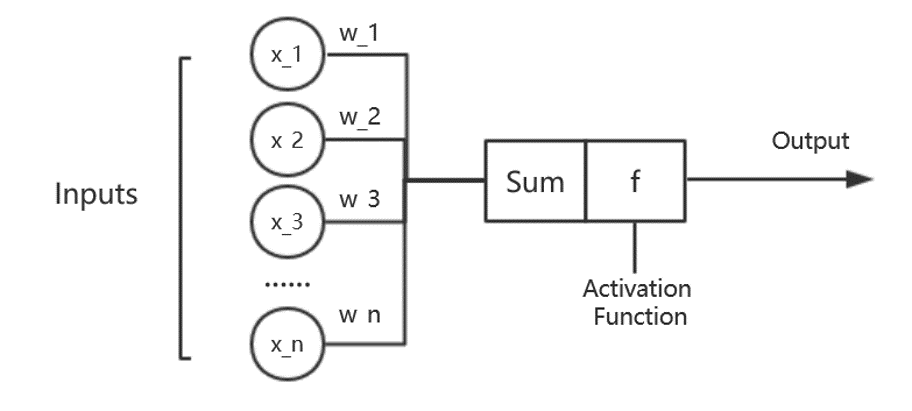
\includegraphics[width=10cm,height=4cm]{Figures/Chapter03/AN.PNG}
\caption{人工神经元结构}
\label{fig3-AN}
\end{center}
\end{figure}


人工神经网络靠的是正向和反向传播来更新神经元,从而形成一个完整的神经系统,本质上,这是一个能让计算机处理和优化的数学模型。而生物神经网络是通过刺激,产生新的联结,让信号能够通过新的联结传递而形成反馈。那么神经元是如何学习事物特征的呢?人工神经元的学习过程被视为一个权重优化不断迭代的结果。也由此也确定这种学习类型是监督学习。权重的调整,以训练数据为基础,结果是已知的类型[也即监督学习]。优化权重是为了最小化损失函数,最优权重可以用来计算未知数据预测结果的类别概率。%这也表明对预期结果的概率。
这里面涉及权重函数的优化和随机梯度算法。从关系上说,就是通过随机梯度下降实现权重优化。

一开始模型只是简单的线性回归模型,作用是为了实现分类。这种类型模型是一个简单神经元的模型,而是线性模型。这样对非线数据的处理就要考虑新的问题。故而引入激活函数(Activate Function)。从另一个侧面考虑了人工神经元会自动学习事物特征,自然而然涉及随机梯度下降算法(或随机梯度上升算法)。下面先介绍简单回归模型Percepton,理解其中的激活函数等,再通过Adaline 理解随机梯度下降算法\ref{fig3-PA}。

\begin{figure}
\begin{center}
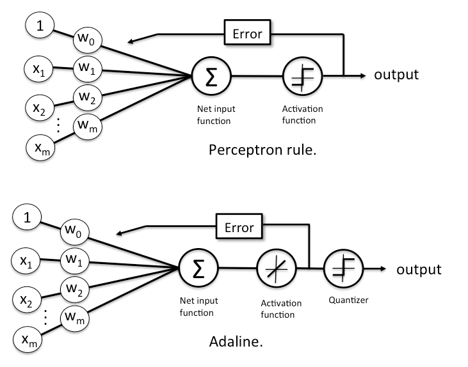
\includegraphics[width=10cm,height=8cm]{Percepton-Adaline.PNG}
\caption{人工神经元模型规则}
\label{fig3-PA}
\end{center}
\end{figure}

在感知机(Percepton)模型中,这里可以看做一个线性回归模型。
对于线性回归问题,优点:结果易于理解,计算上不复杂。缺点:对非线性的数据拟合不好。适用数据类型:数值型和标称型数据。
假设寻找找到最佳拟合直线:y=0.1*x-0.3, 0.1和-0.3 称为回归系数。这样一条直线的确立也是对二分类问题的解。利用线性回归得到最佳拟合曲线,其实求回归方程中的系数,就可以得到回归方程。一般使用的求解方法是最小二乘法。而得到最佳拟合曲线一旦得到,对于新的数据的分类问题,自然而然能够预测该数据属于哪个类别,这也是回归作为分类学习算法的原理。

$X$ =
$\left(
  \begin{array}{ccccc}
    x_{11} & x_{12} & \cdots & x_{1d} & 1 \\
    x_{21} & x_{22} & \cdots & x_{2d} & 1 \\
    \vdots & \vdots & \ddots & \vdots & \vdots \\
    x_{m1} & x_{m2} & \cdots & x_{md} & 1 \\
  \end{array}
\right)
$
=
$\left(
   \begin{array}{cc}
     x^{T}_{1} & 1 \\
     x^{T}_{2} & 1 \\
     \vdots & \vdots \\
     x^{T}_{m} & 1 \\
   \end{array}
 \right)
 $

再把标记也写成向量形式 $\bf{y}$ = ($y_{1}$;$y_{2}$;$\ldots$;$y_{m}$), 则得到的解便是回归系数。

上面的问题是一个线性数据模型,可以认为该模型的传递函数为恒等式(即保持数值不变);直接输出结果。当数据是非线性关系的时候,就考虑新的模型处理数据。引入Logitic 回归。而对Logistic回归而言,传递函数是Sigmoid函数。传递函数即为激活函数。Logitic 回归模型解决非线性二分类问题。那么多分类问题就需要用softmax函数。Softmax分类是对Logistic回归在多个不同的值上的推广。 Logistic回归的激活函数是 Sigmoid函数,而Softmax的激活函数是 一个叠加的Sigmoid函数。
\begin{figure}[htbp]
\begin{center}
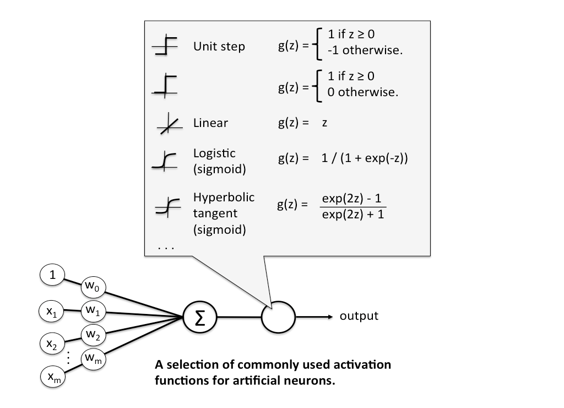
\includegraphics[width=12cm,height=10cm]{AFunction.PNG}
\caption{激活函数}
\label{fig3-AF}
\end{center}
\end{figure}

那么权重函数是如何优化?$W $代表特征权重(Weight),首先给一个随机初始值(可以相等,也可以考虑用截断的高斯分布随机值)。这里假定对数据建模的公式为$y_i = W_i*X_i + bias_i$,bias作为偏差值(也是阈值)决定最后y的分类结果。如果模型的学习结果跟实际结果相同,则这个权重是非负比例的特征权重,所以不对权重进行调整,但是如果模型的学习结果与实际结果相反,则这一次学习对权重需要有所调整。推导如\ref{eq3-weight}所示。

\begin{align}
 W     &:=\  W\ +\ \Delta W     \label{eq3-weight}  \\
 \Delta W_j &=\  -\eta \frac{\partial J}{\partial W_j}\ \nonumber \\
 &=\  \ -\eta \sum_i (target^{(i)} - output^{(i)})(-x_j^{(i)})  \nonumber     \\
 &=\  \eta \sum_i (target^{(i)} - output^{(i)})x_j^{(i)}
\end{align}
其中 $J$是目标函数(成本函数),也是用来判别结果是否来调整权重的损失函数。$\eta$是学习率,一般学习率设置需要适当,不然会导致取不到最优值,也可能会陷入局部最优值。
\begin{align}
  \frac{\partial J}{\partial W_j} &=\  \frac{\partial}{\partial W_j} \sum_i \frac{1}{2} (target^{(i)} - output^{(i)})^2\ \nonumber \\
 &=\    \frac{1}{2}  \sum_i \frac{\partial}{\partial W_j} (target^{(i)} - output^{(i)})^2   \nonumber     \\
 &=\  \frac{1}{2}  \sum_i 2 * (target^{(i)} - output^{(i)})\frac{\partial}{\partial W_j} (target^{(i)} - output^{(i)}) \nonumber \\
 &=\   \sum_i  (target^{(i)} - output^{(i)})\frac{\partial}{\partial W_j} (target^{(i)} - \sum_j w_j x_j^{(i)})  \nonumber \\
 &=\   \sum_i (target^{(i)} - output^{(i)})(-x_j^{(i)})
\end{align}

总结来说,人工神经元通过卷积核映射学习数据特征,通过正向或反向传播传递误差,在随机梯度下降算法支持下优化损失函数,从而更新权重函数,进而实现对数据特征自动学习。

\subsection{卷积神经网络}
从提出人工神经元,到提出卷积神经网络。自1998年Lecun等人\cite{lecun2015lenet}实现第一个运算完整的卷积神经网络模型LeNet-5模型,在这之后网络基本结构就相对固定下来了。后续在(Large Scale Visual Recognition Challenge)中提出了更多更复杂有效的模型,按照提交时间排序为AlexNet(2012)\cite{krizhevsky2012imagenet},
VGG-16(2014),
Inception-v1(,
Inception-v3,
ResNet-50(
Xception
Inception-v4
Inception-ResNets
ResNeXt-50(2015)
这些模型都在不同应用比赛中名列前茅。

% definition
卷积神经网络 ( Convolution neural network, CNN ) 由一组非线性函数映射或者仿射变换函数组成,通过学习训练数据,得到由训练集定义的经验分布,从而用来预测未来数据的概率分布函数等等。之所以称为“卷积神经网络”,表明该神经网络中至少一层使用了卷积( convolution ) 运算。卷积网络会提供一些工具,在具体环境中选择相应的工具给出通用的准则很有必要。卷积神经网络结构的研究进展发展很迅速,以至于针对特定基准(benchmark),没多久就会公开一个新的最优的网络结构。

对于一般的二分类问题而言,卷积神经网络通过学习这两个类别数据的不同之处来得到一个“分类器”,在应用这个“分类器”,之后能得到描述两个分布的概率密度函数,我们一般只关心正样本数据的概率分布。

%更细致地来说,从感知机(Perceptron)发展到卷积神经网络,其基本原理是在高维空间中,寻找一个最优的分割面,也被称为边界超平面,这个分割面能将不同类别的数据集分离。但是最开始的“MP"模型或感知机,他们只针对线性可分或近似线性可分的数据集有很好的效果,对于线性不可分的数据,后者渐渐发展激活函数,可以部分解决这种问题。





%\subsection{卷积神经网络结构}
卷积神经网络一般是针对图像处理,其特点表现在卷积层的作用,卷积层类似于自动提取信号特征,再借助激活函数做降维或者分类。一般的卷积神经网络有以下四层,第一是输入层,处理数据格式;第二是卷积层,自动提取特征;第三是池化层,降低数据维度,提取更高代表性特征,第四是全连接层(类似多层感知机),输出结果。这种结构下一定会卷积层,中间的隐层层的构建取决于数据构建与结果分析。

\begin{figure}[htbp]
\begin{center}
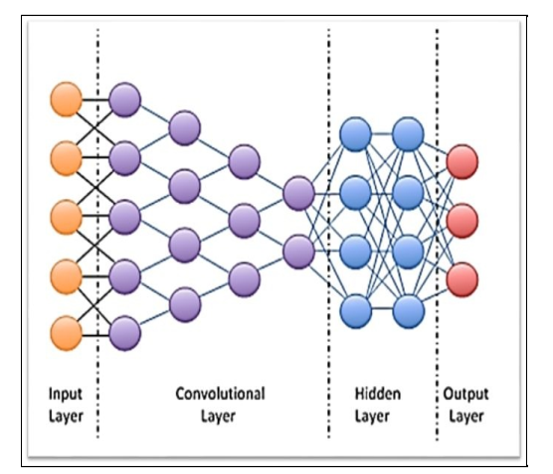
\includegraphics[width=8cm,height=5cm]{CNN.PNG}
\caption{CNN结构;图片来自\cite{zaccone2018deep}}
\label{fig3-CNN}
\end{center}
\end{figure}

所以一般卷积神经网络的层次结构分为:输入层-卷积层-激励层-池化层-(迭代)-全连接层-输出层。下面分层功能进行解释。

%\subsubsection{卷积层}
卷积层一般用于自动提取特征,其中卷积运算是理论上是对两个实变函数的一种数学运算(operation)。在一些数据上,比如时间序列函数,时间上越近的测量结果越相关。故而会采取某种运算使得对最近的测量结果赋予更高的权重,例如采用加权平均操作。实现这种运算可以得到卷积的定义。卷积运算通常用"*"表示。
$$s(t)=(x*w)(t)$$

一般而言,卷积的第一个参数(即公式中的“x”)通常是输入(input),第二个参数(函数“w”)叫做核函数(kernel function)。输出一般被称作特征映射(feature map)。
具体举例来说,
假设输入的图像数据为5*5=25的图像;卷积核为3*3=9的矩阵,那么移动卷积核过程中提取出来的特征是3*3=9的特征矩阵。
\begin{figure}[htbp]
\begin{center}
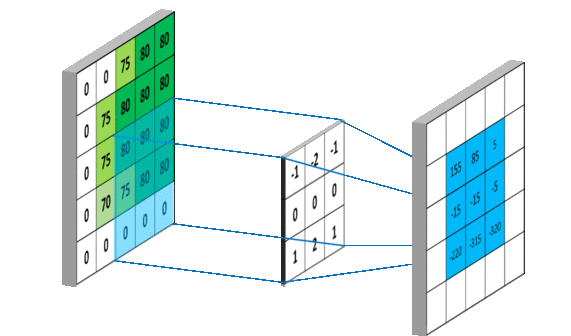
\includegraphics[width=12cm,height=6cm]{cl.PNG}
\caption{卷积层;图片来自\cite{Robinson2018}}
\label{fig3-CL}
\end{center}
\end{figure}

在机器学习应用中,输入通常是多维数据,而核函数是由学习算法优化得到多维数组的参数。卷积运算不仅仅可以在一个维度上做运算,也可以多维做运算,而且可以实现可交换。

%卷积层实现自动提取特征功能。
实际训练过程中,
每层卷积层由若干卷积单元组成,每个卷积单元的参数都是通过反向传播算法优化。卷积运算的目的是提取输入数据的不同特征,第一层卷集层可能只能提取一些低级的特征,如边缘、线条、和角等层级,更高层的网络是从底层的特征中迭代提取出来的,称为更加复杂的特征。
    %在卷积层中提取特征我们需要用到卷积核,卷积核就是一个矩阵。

%\subsubsection{池化层}
%池化层实现特征的表示与降维。
池化层,也称为下采样,与之相对的是上采样(卷积层),主要用于特征降维,压缩或减少数据和参数的数量,减少过拟合,同时提高模型的容错性和训练速度。池化层的输入一般源于上一个卷集层的输出,它的作用是保留主要的特征,同时减少下一层的参数和计算量,防止过拟合。如保持某种不变性,平移、选旋转、尺度缩放、加噪声等等。

 \begin{figure}[htbp]
\begin{center}
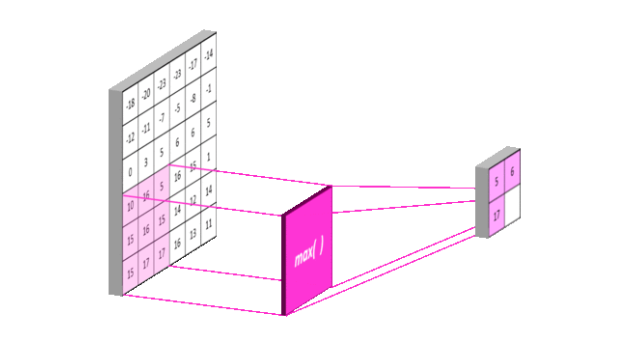
\includegraphics[width=12cm,height=6cm]{pl_2.PNG}
\caption{池化层;图片来自\cite{Robinson2018}}
\label{fig3-PL}
\end{center}
\end{figure}
一般采用的方法有最大池化和均值池化。(最大值采样、均值采样)选择最大池化层和平均池化层的区别。最大池化层是提取最明显的特征,平均池化 层是顾及每一个像素,取平均值。
 \begin{figure}[htbp]
\begin{center}
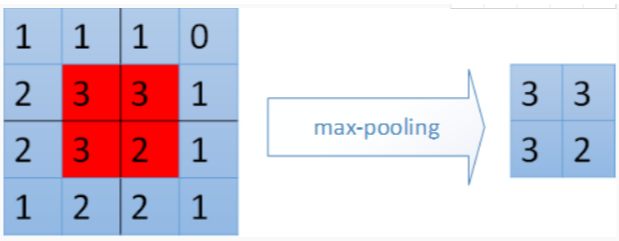
\includegraphics[width=8cm,height=4cm]{maxSampling.PNG}
\caption{最大池化:图片来自\cite{Robinson2018}}
\label{fig3-MS}
\end{center}
\end{figure}
 \begin{figure}[htbp]
\begin{center}
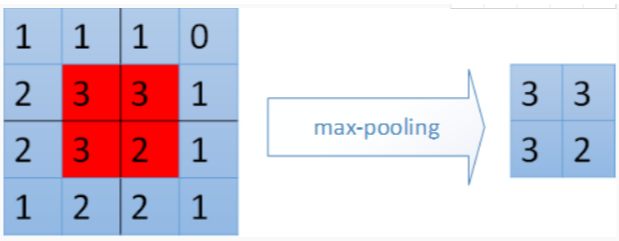
\includegraphics[width=8cm,height=4cm]{maxSampling.PNG}
\caption{均值池化;图片来自\cite{Robinson2018}}
\label{fig3-MaxS}
\end{center}
\end{figure}

%\subsubsection{全连接层}
全连接层的作用就是类似于多层感知机。把之前通过多层神经元映射得到的特征映射图结合起来,且经过激活函数,多层的神经元激活使得当前最优且线性不可分的特征表示 通过非线性的激活操作,使得数据(以特征表示)在输出层变成线性可分。全连接层一般为两到三层,神经网络的性能就到达一定的极值[黄安埠《深入浅出深度学习(原理剖析与python实践]

%\subsubsection{激活函数}
无论经过卷积成还是池化层,出来的数据都是连续性的,假设数据的范围在0与1之间,那么可以是0和1之间的任何数。线性化的模型不能直接解决类似“异或”这种非线性化的问题。
    
而选取激活函数是用来加入非线性因素的考量,因为线性模型的表达能力不够。对于时间序列,我们也采用的是卷积方式来处理,对每个时间观测值都赋予一个权值,这个操作显然是线性的。但是对于我们的样本来说不一定是线性的,为了解决这个问题,我们可以进行线性变换,或者引入非线性的因素解决问题,即隐藏层中激活函数的引入。非线性的激活函数使得复杂的非线性数据集也能被处理,且切实提高了模型的学习和表示能力。经过激活函数处理后,模型中神经元会被赋予不同权重,权重意味这该神经元是否被激活,那该神经元所表示的数据的特征就会不同程度地被采纳,从而实现模型能自动提取特征的作用。

% 举例说明 激活函数的作用
举例来说,Lee等人在音频的时间序列里,通过时频图来展示一个音频数据,经过激活函数后的特征权重被调整为(0,1)之内的值,且遵循sigmoid函数的特性。不同的权重意味着对不同特征的重视程度,多种特征的组合之后得到最优特征表示,达到关键信息中自动提取关键特征的作用。
\begin{figure}[htb]
 \centering
 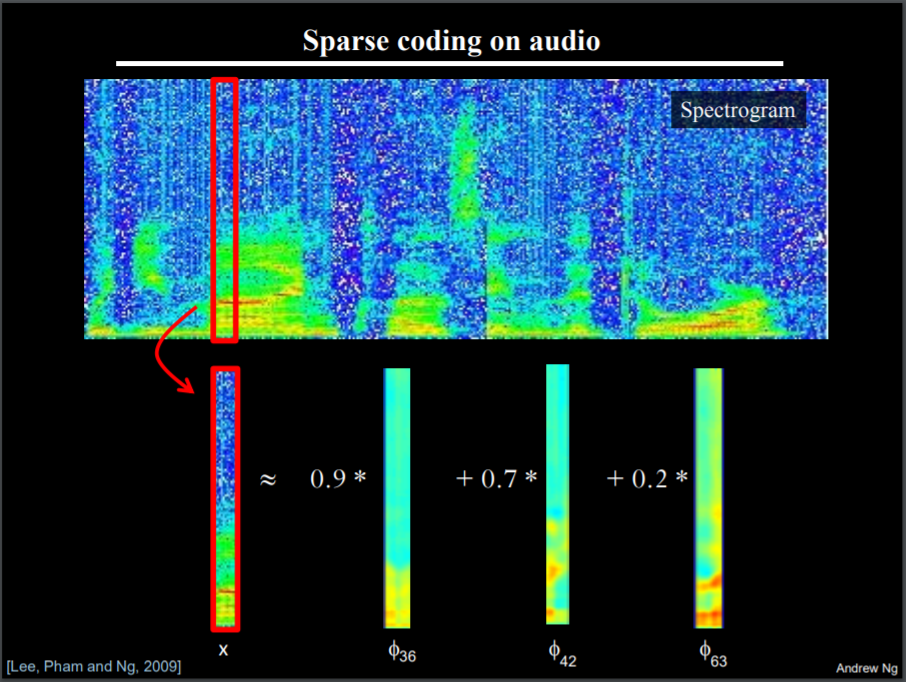
\includegraphics[width=.8\linewidth]{SparseRepresent.png}
    \caption{\label{fig:SR}音频数据时频图的自动提取特征过程}
\end{figure}



在卷积神经网络中,Alex等人\cite{krizhevsky2012imagenet}研究表明Relu函数比传统激活函数(如sigmoid函数)优,能够缓解训练过程中的梯度消失问题。具体表达式如式(\ref{eq3-relu})所示,。
\begin{equation}
ReLU(x)=
\begin{cases}
x& \text{if\ x $>$ 0}\\
0& \text{if x $\leq$ 0}
\end{cases}
\label{eq3-relu}
\end{equation}


\begin{comment}
\subsection{数据集准备}
%\subsubsection{数据集准备}

在机器学习算法中,一般会准备3种数据集,分别是训练数据集、验证数据集和测试数据集。他们三个数据集完全不同,他们的作用也各不相同。训练数据集顾名思义用来训练神经网络算法,使得神经网络算法能够从中学习到数据的特性或特征。而验证数据集则用来检验神经网络学习效果,如果神经网络算法也能够正确辨别验证数据集,证明该算法正走向正确标签的类别,如果不能正确辨识验证数据集,则会用来惩罚该学习过程,使得学习过程能够修正方向。故而训练数据和验证数据一般是独立同分布(Independently Identically Distribution, IID )的数据构成。最后是测试数据集,这个一般是正式应用的数据集打包而成。而且最接近真实应用场景的数据,它一般只经过最少的数据预处理,用于检验前面训练得到的神经网络算法是否具备真实辨识能力和能做到什么样的程度。

在这个过程中,其实假设了真实数据的分布信息蕴含在数据中,但是有时候真实数据量很少,并不能完全分割为三种数据集,且我们并不知道数据真实分部信息。所以采用了模拟的数据集,假设了数据服从更宽泛的分布范围,神经网络算法能从中学习,且能够应该于真实分布的测试数据。故而,我们采用的训练数据要尽可能采用更宽泛的分布模拟数据,用于检验该算法学习效果的验证数据集也采用跟训练数据一样的分布信息。测试数据集采用真实的观测数据或者最接近真实的模拟数据。具体来说,在本论文中,训练数据和验证数据中波形是采用同样随机分布得到所有引力波源参数(如中心黑洞质量都是采用log分布)产生的EMRI波形,而测试数据集则采用天文学模型得到引力波源参数来产生EMRI波形。之后都是以同样方式叠加模拟的高斯噪声,用来作为正样本。在三种数据集中的负样本都是同样方法产生的随机高斯噪声。
\end{comment}

\subsection{循环神经网络}
%\subsubsection{循环神经网络}
循环神经网络(Recurrent Neural Network,RNN)是一类专门用于处理时序数据样本的神经网络,它的每一层不仅输出给下一层,同时还输出一个隐状态,给当前层在处理下一个样本时使用。就像卷积神经网络可以很容易地扩展到具有很大宽度和高度的图像,而且一些卷积神经网络还可以处理不同尺寸的图像,循环神经网络可以扩展到更长的序列数据,而且大多数的循环神经网络可以处理序列长度不同的数据(for 循环,变量长度可变)。它可以看作是带自循环反馈的全连接神经网络。
%其网络结构如下图所示。

\begin{figure}[htbp]
\begin{center}
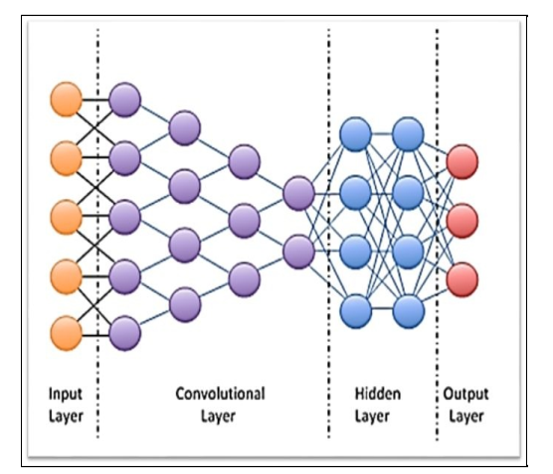
\includegraphics[width=8cm,height=6cm]{CNN.PNG}
\caption{RNN结构;图片来自\cite{zaccone2018deep}}
\label{fig3-RNN}
\end{center}
\end{figure}

长短时记忆网络(LSTM),时序反向传播算法按照时间的逆序将错误信息一步步地往前传递。当每个时序训练数据的长度$T$较大或者时刻$t$较小时,损失函数关于$t$时刻隐藏层变量的梯度比较容易出现消失或爆炸的问题(或称长期依赖问题)。


\begin{comment}
\subsection{探测结果分析}
%描述四种概率
%描述误报率和阈值的计算,比如如何求出来的信噪比大于8
%ROC curve 和efficiency curve

%描述如何计算阈值的过程,这很有分量,但是实际我还没有算出来为什么是20?是由于模板的精度决定的吗?
在信号探测中,检测概率和错误概率是最常需要的计算。目前在我们理论计算过程中,通常假设噪声都是高斯噪声,实际探测过程会是非高斯、非稳态的噪声,但这种需要在实际仪器运行过程中才能评估噪声特性。所以我们还是基于高斯稳态噪声的假设下进行的探测检验。

高斯噪声n(t)顾名思义其数据点特性满足高斯分布,则n分布密度函数为:

$p(n)=\frac{1}{\sqrt{2\pi}\sigma}e^{-(n-\mu_n)^2/2\sigma_n^2}$

公式中$\mu_n$和$\sigma_n^2$分别是噪声的均值和方差。从高斯函数特性也可得到n的累积分布函数(cumulative distribution function, CDF)为:

$F(n)=\int_n^{\infty}p(n)dn = \frac{1}{\sqrt{2\pi}}\sum_n^{\infty}e^{-(n-\mu_n)^2/2\sigma^2_n}
=\frac{1}{2}\frac{2}{\sqrt{\pi}}\sum^{\infty}_{(n-\mu_n)/\sqrt{2}\sigma}{e^{-t^2}dt}$

定义误差函数(error function)
$$
和误差补余函数
$$

则可以把累积分布函数和误差函数以及误差补余函数函数都串联起来。
即高斯噪声n的累积分布函数可以写成:
$F(n)=\frac{1}{2}erfc(\frac{(n-\mu_n)}{\sqrt{2}\sigma_n})=\frac{1}{2}[1-erf(\frac{(n-\mu_n)}{\sqrt{2}\sigma_n})]$

\end{comment}
%\section{参数估计}
%\clearpage

\chapter{天琴对EMRI信号探测初探}

本章将介绍如何利用深度卷积神经网络算法构建天琴探测流水线,用以进行EMRI信号探测。主要内容分为四个部分。首先是数据的准备工作,包括信号建模,天琴仪器噪声建模,数据清洗等预处理工作;第二,进行数据的验证,验证模拟数据的正确性;第三,构建卷积神经网络模型,包括模型结构,目标函数及优化函数的选取等;最后,评估探测模型的性能和分析结果。




\section{准备数据}
%% 1. 介绍noisy signal 构造和noise only 样本的构造
%% 2. 正负样本的验证工作
%% 3、各个数据集的准备工作
在机器学习算法中,一般会准备3种数据集,分别是训练数据集、验证数据集和测试数据集。他们三个数据集完全不同,他们的作用也各不相同。训练数据集顾名思义用来训练神经网络算法,使得神经网络算法能够从中学习到数据的特性或特征。而验证数据集则用来检验神经网络学习效果,如果神经网络算法也能够正确辨别验证数据集,证明该算法正走向正确辨识数据类别的方向上。如果不能正确辨识验证数据集,则会用来惩罚该学习过程,使得学习过程能够修正方向。故而训练数据和验证数据一般是独立同分布(Independently Identically Distribution, IID )的数据构成。最后是测试数据集,这个一般是正式应用的数据集打包而成。而且最接近真实应用场景的数据,它一般只经过最少的数据预处理,用于检验前面训练得到的神经网络算法是否具备真实辨识能力和能做到什么样的程度。

在这个过程中,其实假设了真实数据的分布信息蕴含在数据中,但是有时候真实数据量很少,并不能完全分割为三种数据集,且我们并不知道数据真实分布信息。模拟的数据集假设服从更宽泛的分布范围,神经网络算法能从中学习,且能够应用于真实分布的测试数据。故而,我们采用的训练数据要尽可能采用更宽泛的分布模拟数据,用于检验该算法学习效果的验证数据集也采用跟训练数据一样的分布信息。测试数据集采用真实的观测数据或者最接近真实的模拟数据。具体来说,本文训练数据和验证数据中波形是采用同样随机分布得到所有引力波源参数(如中心黑洞质量都是采用log分布)产生的EMRI波形,而测试数据集则采用天文学模型得到引力波源参数来产生EMRI波形。之后都是以同样方式叠加模拟的高斯噪声,用来作为正样本。在三种数据集中正负样本各占一半,且负样本都是采用天琴噪声曲线的高斯噪声。



%按照前面关于卷积神经网络算法的介绍,这需要准备三种数据集,
概括来说,
一个是训练数据集,该数据集的大小一般没有上限,样本数量越充分,就越能更多表示EMRI信号的特点;一个是验证数据集,一般采用训练数据集大小的10\%,用于反馈训练效果;第三个数据集是测试数据集。三种数据集的准备过程基本完全一样,除了训练数据和验证数据会使用数据增强技术增加样本数量。
%以某个数据集的某个数据构建用以说明流程。
取训练数据的构建来描述数据的准备过程,数据准备工作基本流程如图\ref{fig:data_prep}
所示。
\begin{figure}[htbp]
 \centering
 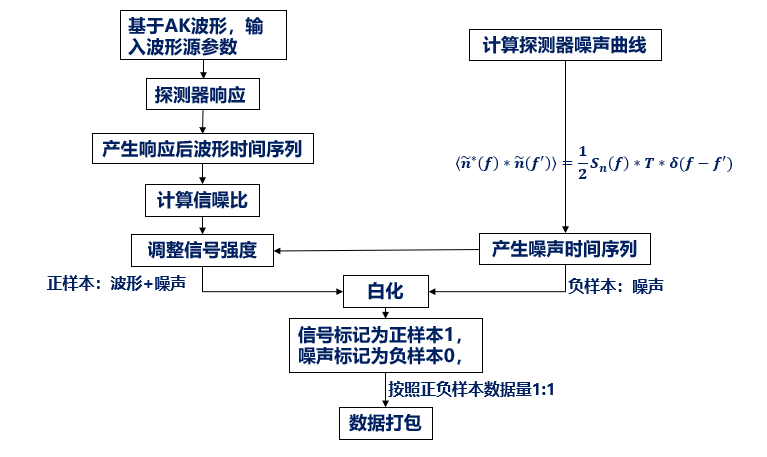
\includegraphics[width=1.1\linewidth]{data_prep}
    \caption{\label{fig:data_prep}训练数据准备流程图}
\end{figure}


%% targets: 由天琴噪声曲线产生高斯噪声

第一,介绍EMRI信号建模。采用AK波形来描述EMRI信号,需要设置14个物理源参数,如中心黑洞质量$\bf{M}$,小致密天体的质量$\bf{m}$等14个参数。在训练数据中,中心黑洞质量满足log分布($\sim log[10^4,10^7]M_\odot$),小致密天体的质量为10$\bf{M_\odot}$,其他的参数都服从均匀分布,具体源参数设置如表\ref{tab:AKW-sources}所示。
\begin{table}[htbp]
    \caption{\label{tab:AKW-sources}AK波形模型源参数取值范围}
    \wuhao
    \begin{tabularx}{\linewidth}{c|c|X<{\centering}}
        \hline
        参数符号 & 参数物理含义 &取值范围 \\ \hline
        M  & 中心黑洞质量 & log distribution[$10^4M_{\odot},10^7 M_{\odot}$]\\ \hline
        $\mu $ & 致密小天体  & 10$M_{\odot}$\\ \hline
        $a=S/M^2$ & 中心黑洞自旋 & uniform [0.5,1] \\ \hline
        $e_{lso}$ & 最内稳定轨道的偏心率值 & uniform [0,0.2]\\ \hline
        $\Phi_0$  & 初始相位 & uniform[$0.0,2*\pi$]\\ \hline
        $\alpha_0$  & 近日点进动角 & uniform[$0.0,2*\pi$]\\ \hline
        $\gamma_0$ & 轨道面进动角 & uniform[$0.0,2*\pi$]\\ \hline
        $\lambda$  & 轨道倾角 & cos($\lambda$)= uniform[-1,1]\\ \hline
        $\nu_{lso}$  & 最内稳定轨道截止频率 & 由$e_{lso}$决定\\ \hline
        $\theta_S$  & 黄道坐标下源的纬度 & uniform[$0.0,2.0*\pi$]\\ \hline
        $\phi_S$  & 黄道坐标下源的经度 & cos($\phi_S$)=uniform[$-1.0,1.0$]\\ \hline
        $\theta_K$  & 黄道坐标下中心黑洞自旋的纬度 & uniform[$0.0,2.0*\pi$]\\ \hline
        $\phi_K$  & 黄道坐标下中心黑洞自旋的经度 & cos($\phi_K$)=uniform[$-1.0,1.0$]\\ \hline
        $D_L$  & 初始光度距离 & $4.418*10^8$ [$\rm Psec$]\\ \hline
    \end{tabularx}
\end{table}

故而基于所有物理源参数的分布,可产生随机的源参数,采用AK波形得到模拟的EMRI源信号。之后基于探测器迈克尔逊低频近似响应,得到天琴响应后的EMRI信号。具体天琴响应方程式如公式所示。天琴响应主要影响极化角、方位角和多普勒平移的计算。

%说明极化角和多普勒平移的实际计算。
关于极化角$\psi_S$计算,$\bf{S}$表示源坐标下。具体公式计算如所示,实际带入天琴响应函数时,需要进行坐标转换,跟源方位角一样,都采用探测器坐标表示。
\begin{equation}
\tan \psi_S = \frac{\hat{L} \cdot \hat{z}-(\hat{L}\cdot \hat{z})(\hat{z}\cdot \hat{n})}{\hat{n}\cdot (\hat{L}\times \hat{z})}
\end{equation}
其中$\hat{L}$是轨道角动量方向的单位向量,$\hat{n}$是相对引力波波源传播反方向的单位向量。根据文献\cite{luo2016tianqin}, 天线响应函数中$\theta_S$不随时间变化,而$\phi_S$随时间变化。当$\phi_S$转换到探测器坐标系下,天琴的绕转周期为1天,即$\omega=2\times 10^{-5} rad/s$,则$\bar{\phi}(t)=\bar{\phi_0}+\omega t$。极化角$\psi_S$也会由于轨道角动量随时间变化而发生变化。
%多普勒平移
此外,因为探测器会随地球质心每年的周期运动而引入一个多普勒平移项,故而在时间域响应的信号上,相位多添加一项。则$\bar{\phi}_{\rm Doppler} (t)=\bar{\phi_0} +2\pi t/ T$,$\bar{\phi_0}$代表探测器在初始时刻$t=0$的位置,$T=1 year$表示地球绕太阳的轨道周期。

%说明EMRI波形产生速度慢,需要提前产生,计算一下产生效率的问题。
由于EMRI波形产生速度相对而言较慢,故而我们产生了$10^6$个模拟EMRI波形存储在硬盘。

%利用天琴噪声曲线产生模拟仪器噪声。
第二,产生模拟噪声。基于天琴探测器噪声曲线,产生高斯平稳的噪声序列。即利用噪声功率谱定义,产生模拟高斯噪声。
\begin{equation}
<\tilde{n}(f)\tilde{n}(f')>=\frac{1}{2}S_n(f)\times T_{obs} \times\delta(f-f')
\end{equation}
其中$\tilde{n}$表示频率域的噪声,$S_n(f)$是天琴噪声单边功率谱密度,具体表达式如公式表示,由文献\cite{luo2016tianqin}给出。$T_{obs}$表示观测时长。
\begin{equation}
S_n(f)=\frac{1}{L^2}\lbrack \frac{4S_a}{{(2\pi f)^4}} (\frac{1+10^{-4}Hz}{f}) + S_x \rbrack \lbrack 1+ 0.6((\frac{f}{f_*})^2)\rbrack
\end{equation}
$S_a$ 是加速度噪声, $S_a^{1/2}=1\times 10^{-15}m s^{-2}/\sqrt{Hz}$, $S_x$ 是位置噪声且 $S_x^{1/2}=1\times10^{-12}m/\sqrt{Hz}$, $f_*$ 是噪声极限且 $f_* =\frac{c}{2\pi L}$,$L$是探测器轨道臂长且$L=1.0\times 10^5 km$,$c$是光的传播速度。

产生频率域的噪声之后,由逆傅里叶变换可得到时间域的噪声序列。纯粹的噪声可以充当负样本,被标记为``0"。在时间域上,正样本由EMRI波形叠加噪声得到。并且正负样本都会经过白化操作并进行归一化。具体的白化操作表示如公式所示。
\begin{equation}
s = \frac{s}{\sqrt{S_n(f)}}
\end{equation}
其中$s$表示就是数据,如果是纯噪声,则$s(t)=n(t)$;如果数据含有信号,则$s(t)=h(t)+n(t)$,$h(t)$为时间域的EMRI信号模板。

%调整信噪比
第三,调整一个某信号的信噪比。由于EMRI信号非常复杂,显然其信号强度越弱,信噪比就可能越低,探测就越困难。为了简化EMRI信号探测问题,我们选取信噪比满足[50,120]的均匀分布的EMRI信号来构造数据集的样本。这里面涉及调整信噪比的操作。

当给定一个初始光度距离$D_L$和其他随机的物理源参数,能够产生一个初始响应后的EMRI信号,利用理想信噪比公式计算得到初始信噪比$\rho$。从均匀分布[50,120]中产生一个随机数$\rho_a$,由于波源距离与引力波强度成反比的关系,我们可以通过调整距离使得该波形强度调整为满足某信噪比的波形强度,即该波形新距离调整为$D_{\rm new}=\frac{\rho \times D_L}{\rho_a}$。理想信噪比的计算公式如\ref{exp:optimal_snr}所示,由于天琴可视作两个迈克尔逊干涉仪,则两个探测器对某一个引力波信号的总信噪比等于两个单独的信噪比的平方和后开方。
\begin{equation}\label{exp:optimal_snr}
\rho^2 = 4 \sum \frac{h(f)^2}{S_n(f)} df
\end{equation}

以上就是构建数据集中正负样本的基本过程,训练数据和验证数据是完全一样的准备过程,只是采用不同的源参数分布种子产生随机数,得到不同波形。但考虑由此得到数据集总数还不充分,还会通过数据增强技术增加样本数量。而测试数据集则没有用数据增强技术,但会采用其他源参数分布和波形模型用以构造不同的正样本,对最终的信号探测模型进行评估。


%数据增强
在训练数据和验证数据的准备上,尽管我们采用多进程产生波形,并且利用天河超级计算机的计算资源,产生EMRI波形的数量需求仍有所欠缺,而且考虑到存储的顾虑,因而我们也采用了数据增强技术,增加了训练数据和验证数据的正样本数量,用以增强探测模型的鲁棒性和避免卷积神经网络模型训练过程中出现过拟合问题。
具体的做法是,产生一个EMRI波形,训练过程中会产生 $n$个 噪声时间序列,且叠加到同一个EMRI波形上,则可以构造$n$个正样本(
$1\times n$),又免去存储的顾虑。
在本文实验中,采用$n=8$。实际上,数据增强技术在其他领域也发挥了举足轻重的作用,可详细参考文献[data-aug]

%其他源参数分布、波形模型
在测试数据集的准备上,会构造不同测试数据用以评估得到探测CNN模型的性能且不使用数据增强技术。测试数据集正负样本各一半。
%第一种,基于AK波形,采用与训练数据相同的源参数分布和信噪比分布($SNR \sim U[50,120]$) 产生的EMRI波形。第二种,基于AK波形,采用与训练数据相同源参数分布,但更广范围的信噪比分布,产生EMRI波形。第三种,基于AK波形,采用源参数的天文学分布,产生EMRI波形。第四种,基于AAK波形,采用与训练数据相同源参数分布和信噪比分布,产生EMRI波形。
其中负样本都是采用天琴噪声曲线产生的高斯噪声,满足独立同分布;而正样本模拟信号会由于模拟波形不同而不同,其样本概率分布会有所差异。模拟波形的不同影响因素有两种。一是波形模型,AK模型和AAK模型。二是波源物理参数,模拟联合概率分布(simulated joint probability)和源天文学分布(astronomical model)。其中还需要特别考虑模拟信号的强度不能太弱(信噪比),一方面在天文学模型中利用共动体积撒点得到光度距离,假如得到波源信噪比小于50,则丢弃;另一方面模拟源参数分布中可利用理想信噪比的计算来调整波源光度距离,从而选择合理的模拟波形。在这其中信噪比分布有均匀分布[50,120],也有从[10,130]取固定某个信噪比。

与训练数据相比较,基于以上两种影响模拟波形的因素可以构造6种测试模拟信号,具体模拟信号的情况如表\ref{tab:test-wave}。与此同时,也会产生跟模拟信号相同数目的模拟噪声样本。
\begin{table}[!htbp] 
\caption{测试数据集情况}  
\wuhao
\begin{tabularx}{\textwidth}
	{p{0.05\textwidth}%
	p{0.07\textwidth}%
	p{0.5\textwidth}%
	p{0.1\textwidth}%
	p{0.15\textwidth}}  % 10cm 減去前兩個欄位寬度後,剩下的通通給  
\hline                      % 第三欄位使用,文字超出的部份會自動折行  
类型 & 波形模型  & 源参数分布   & 模拟信号数目 & 评估指标  \\  
\hline  
1  & AK & 模拟联合概率分布, 信噪比服从均匀分布[50,120] & 500  & 混淆矩阵, ROC曲线  \\ 
2  & AK & 天文学模型 M12,信噪比大于50 & 500  & ROC曲线 \\ 
3  & AAK & 模拟联合概率分布, 信噪比服从均匀分布[50,120] & 500  & ROC曲线  \\ 
4  & AK & 模拟联合概率分布,固定信噪比[10,130] & 1000  & 有效性曲线\\ 
4  & AK & 固定MBH质量 $[10^4, 10^7M_{\odot}]$ & 1000  & 有效性曲线\\
5  & AK & 固定MBH自旋 $[0.0, 0.98]$ & 1000  & 有效性曲线\\
6  & AK & $\rm MBH\ 10^6M_{\odot},\rm spin\ 0.8$,固定红移 $[0.1,0.35]$ & 1000  & 有效性曲线\\
\hline  
\end{tabularx} 
\label{tab:test-wave} 
\end{table}  



\section{数据验证}
% 时间域高斯噪声满足高斯分布,且得到的时频图满足卡方分布。
在上一节的工作中,数据的准备工作就已经完成,但是数据质量决定了真实探测模型的起步和关键,所以数据验证工作就尤为重要。EMRI信号的验证通过计算信噪比和频率域图像来进行。噪声验证通过不同形式数据满足不同的分布特性来进行。

%展示一个数据样本:A和E画在同一个子图上
目前数据的正负样本如图和图所示。在时间域上,正样本由中心黑洞$10^6 M_{\odot}$-小天体$10 M_{\odot}$的双星系统得到EMRI信号构造而成。而负样本是纯噪声时间序列。白化前,负样本满足高斯分布(0,sigma),白化后,负样本满足N(0,1)的高斯分布。
\begin{figure}[!htbp]
 \centering
 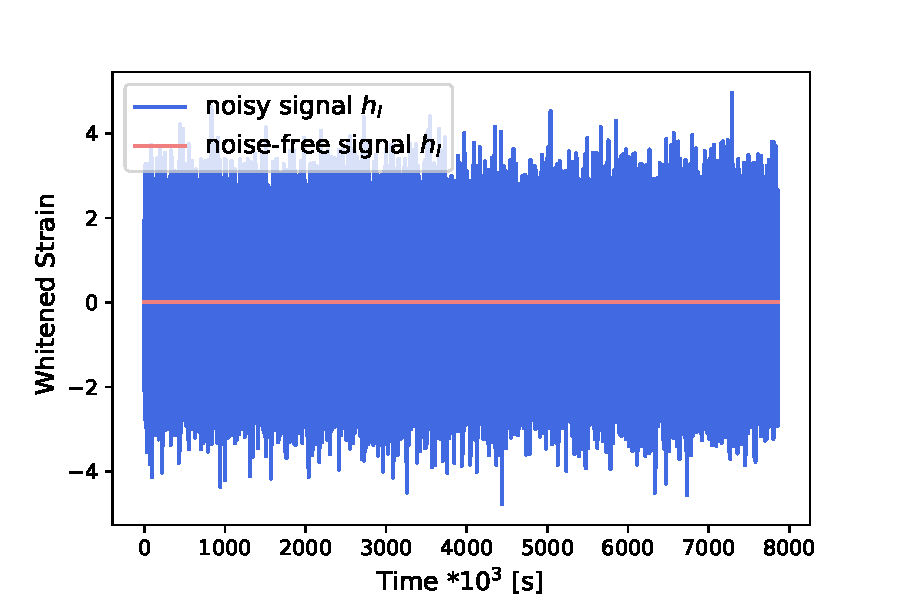
\includegraphics[width=.6\linewidth]{input-data-20210315.pdf}
    \caption{\label{fig:input-data}白化后的模拟信号样本和没有叠加噪声的模拟信号白化后的样本。天琴能够响应得到两个正交模拟信号,将其都经过白化操作,打包成一个正样本,数据维度为$(2 \times 262144)$}
\end{figure}



%高斯分布
以某一个时间域的噪声时间序列为例,白化前后都满足高斯分布,但两个高斯分布的标准差是不一样。
%开方分布
将时间域上的噪声用时频图进行转换,其功率值满足卡方分布,如图所示。自此验证了噪声模拟工作的正确性。

%在信号的模拟上,
在EMRI模拟信号的验证上,即验证波形的准确性。由于AK波形和AAK波形分别由文献\cite{chua2015improved}及其开源代码给出,主要添加探测器天线响应,我们通过取特定的方位角方式验证了响应函数的正确性,其中包括验证坐标系转换等工作。最后通过频率域图像,展示波形的正确性。将天琴的灵敏度曲线和某一个EMRI信号画在同一个图像上,并计算信噪比的合理性。


\section{构建卷积神经网络模型}
%描述模型结构
%训练策略

\subsection{模型结构}
在前人工作的借鉴下\cite{Hunter2018:PhysRevLett.120.141103, George:2016hay}, 设计了初始的神经网络结果,一步步进行训练测试得到了现在的卷积神经网模型。具体模型结构如图所示。一共有9层网络,3层卷积层,3层池化层,2层全连接层,1层输出层。

%模型结构
\begin{figure}[!htbp]
 \centering
 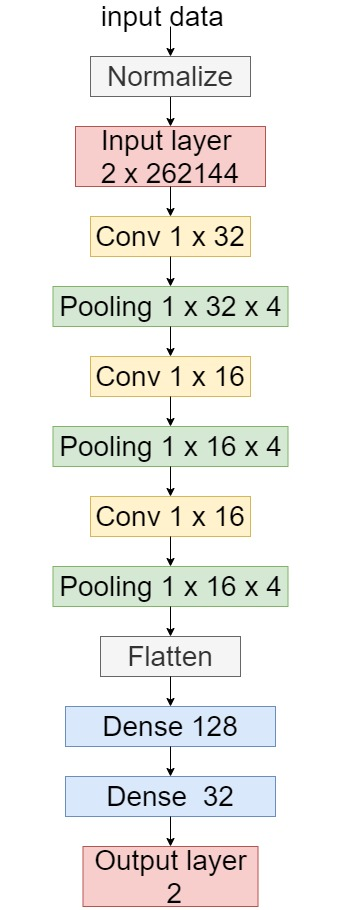
\includegraphics[width=.3\linewidth]{CNN-1}
    \caption[CNN模型结构]{\label{fig:CNN-arch}CNN模型结构。输入数据的维度是$(2 \times 262144)$,将输入数据输入CNN模型的输入层(Input layer)会采用两个通道读入该输入数据。经过三次的卷积(Conv)+池化(Pooling)作用,模型自动提取了特征。经过平铺(Flatten),把所有特征放到同一个维度上来表示。2层完成连接层(Dense layer)实现多层感知机的作用,将特征空间映射到2维的输出空间,从而得到该输入数据属于二分类中某个类别的概率。}
\end{figure}

具体实验环境中,搭建模型的实现和运行过程采用Python3.7、keras2.2.4 和 Tensorflow等软件,相对应的配置硬件环境是GPU Tesla V100 PCIe 16GB,
%CPU Intel Xeon Gold 6140 (72) @2.3,
%Memory 256GB, OS Ubuntu 18.04.4 LTS x86_64。


\subsection{训练过程}
实际训练过程中,模型过拟合问题不可避免[周志华,2016]\cite{zhou2016machine}\cite{ng2013unsupervised},但可以描述当前模型是否能够被接受。为了降低过拟合的影响,本文采用增加样本数据、添加dropout层的方法。具体为,在全连接层之前增加dropout层,参数设置为0.1。在训练数据中采用数据增强方法增加数据量,从而大大降低模型过拟合问题。在目标函数的选取上,选择了二分类交叉熵函数,其公式表示如式所示。
\begin{equation}
L=-\sum_{i=1}^{i=M}[y_i \log \hat{y_i}+(1-y_i)\log(1-\hat{y})]
\end{equation}
其中“L"表示目标函数损失值,``M"表示训练样本数目,$y_i$表示对应样本$i$的真实标签,$\hat{y_i}$对应样本$i$的预测标签。优化算法选择Ndam算法\cite{dozat2016incorporating}。

在训练过程中,由于单个数据大小约为4MB,考虑到内存(256G)和GPU存储容量(16G)的限制,选择了单批次训练数目为56个,设置训练300轮。这也意味着在每一轮训练中,每次会从全部训练数据中随机挑选56个数据进行训练,其中正负样本都各占一半。在具体训练过程中,也同时添加了提早结束训练机制(Early Stopping),假如验证准确率在50轮训练中没有任何提升,则结束模型训练。故而实际训练轮数会有所不同。

模型训练过程中的损失和准确率如图所示,图中展示训练150轮的训练和验证损失值,训练和验证准确率表现。当模型能够学习得到EMRI特征时,则无论是训练和验证损失值都会降低。但模型的实际表现会用测试数据集来评估。

最终训练数据为500000个,验证数据为50000个。

%\section{评估模型}
\section{分析结果}
%验证结果:信号处理分析指标、混淆矩阵、ROC曲线、AUC曲线
%基于本章第一节给出的四种测试数据,对训练得到的CNN模型进行了性能评估,描述的是受过训练以后的模型对未知数据的预测能力,也即泛化能力\cite{li2012s1, li2019s2}。经过训练后的CNN模型也可称为“分类器”或”判别器”。
经过训练后的CNN模型也可称为``分类器"(classifier) 或``判别器”,也称为``判别模型"。判别模型是由数据直接学习决策函数$Y=f(X)$或条件概率分布$P(Y|X)$作为预测模型\cite{li2012s1}。
%不能反映训练数据本身的特性,但它寻找不同类别之间的最优分类面,反映的是异类数据之间的差异。
%直接面对预测,往往学习的准确率更高。由于直接学习P(Y|X)或P(X),可以对数据进行不同维度上的定义特征、抽象化并使用,因此可以简化学习问题。


对训练得到的CNN模型进行了性能评估,描述的是受过训练以后的模型对未知数据的预测能力,也即泛化能力\cite{li2012s1}\cite{li2019s2}。而给出性能评估,就要构造合理评估模型性能的测试数据集,所有的结果都应该基于没有经过训练的测试数据进行检验。因此针对这个分类器的性能评估,实质上就是要分析该模型$Y=f(X)$[$P(Y|X)$]是否合理,从概率角度,我们应该让通过采用更接近真实数据概率分布得到测试样本对模型进行测试。即采用上一节内容中所说的六种测试数据对CNN模型进行测试,并采用相应的评估标准进行展示。


%总结评估指标
参考一般用于信号探测和机器学习算法的评价指标(measure)\cite{li2012s1},本文采用正确率(accuracy),查全率(Recall),查准率(Precision),ROC(Receiver Operating Characteristic)曲线,有效性曲线(efficiency curve)
来分析模型表现。
%误报率(false alarm probability), 漏报率(false missals probality),

对每一个测试数据集,都能得到其经过分类器后的类别结果,也即混淆矩阵(Confusion Metrix)。在这其中,``TP"(True Positive)表示正样本正确分类为正样本的数量,即信号正确分类为信号的数量;``TF"(True Negative)表示为负样本正确分类为负样本的数量,即噪声正确分类为噪声的数量,这两类的结果落在矩阵对角线,对角线的数量越多证明分类模型性能越好。同理可知“FP"(False Positive)表示噪声被错分为信号的数量,``FN"表示信号被错分到噪声的数量。

\begin{table}[!htbp]
\centering
\wuhao
\begin{tabular}{|c|c|c|}
%\begin{tabularx}{\linewidth}{c|X<{\centering}}
\hline
\diagbox{真实标签}{预测标签}&正样本&负样本\\ %添加斜线表头
\hline
正样本&TP&FN\\
\hline
负样本&FP&TN\\
\hline
\end{tabular}
\end{table}



\subsection{准确率、查全率、查准率}
准确率是数据被正确分类的概率,包含信号正确识别为信号,噪声正确识别噪声。具体表达式如公式所示\cite{li2012s1}。
\begin{equation}
\rm Accuracy = \frac{\rm TP+ \rm TN}{\rm TP+\rm FN+\rm FP+\rm TN}
\end{equation}
查准率是正样本被正确分类的数目占全部预测正样本数目的比例。
\begin{equation}
\rm Precision= \frac{\rm TP }{\rm TP+\rm FP}
\end{equation}
查全率,又被称做召回率,表示正样本被正确分类的数目占全部真正正样本数目的比例。
\begin{equation}
\rm Recall = \frac{\rm TP}{\rm TP+\rm FN}
\end{equation}

准确率是描述广泛问题的通用指标,但是由于不同应用场景下会有一些偏好,所以需要同时参考查准率和召回率。在引力波信号探测中,由于引力波信号比较微弱,所以我们更希望不要漏掉可能的引力波信号,故而召回率会更加被偏重考虑。综合考虑查准率和查全率有所侧重,可以引入一个新指标F-score。
\begin{equation}
\rm F-score = (1+\beta^2)   \frac{\rm Precision}{\rm Recall}{\beta^2(\rm Precision + \rm Recall)}
\end{equation}
其中$\beta$是权重系数。当$\beta=1$, 意味着查准率和查全率并重,则该F值是它们两者的调和平均值记为$F_1$,且表达式如下所示。
\begin{equation}
\rm F_1 = \frac{2\times \rm Precision\times \rm Recall}{(\rm Precision+ \rm Recall)}=\frac{2}{\frac{1}{\rm Precision}+\frac{1}{\rm Recall}}
\end{equation}


以跟训练数据独立同分布的1000个测试数据为例,其中500个信号,500个噪声,得到的混淆矩阵如图\ref{fig:cm-iid}所示。%将六种数据类型\ref{tab:test-wave},
得到的汇总准确率等结果指标如表\ref{tab:acc}所示。
\begin{figure}[!htbp]
 \centering
 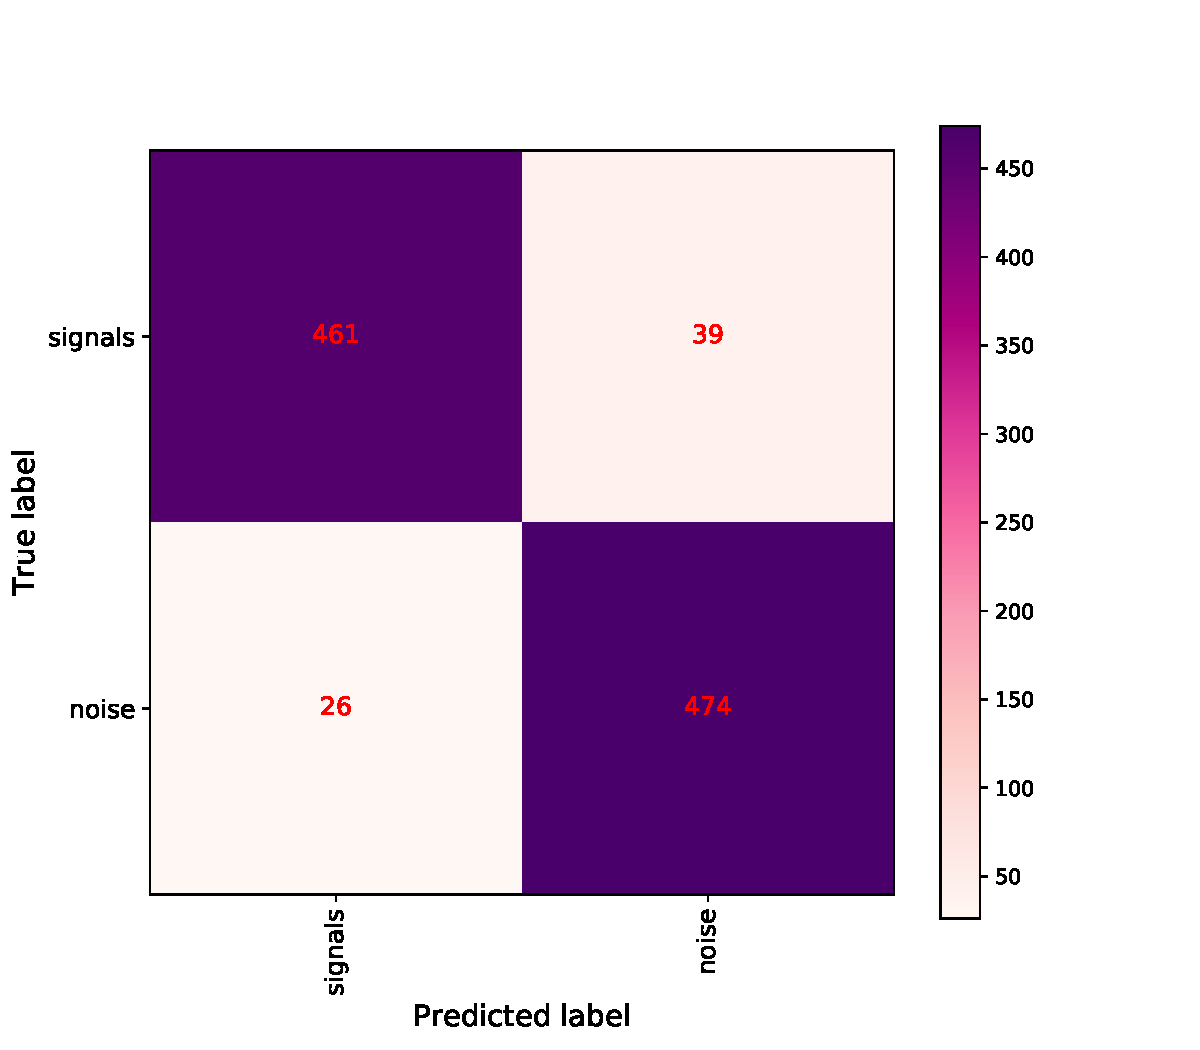
\includegraphics[width=.6\linewidth]{lisatools-AK_cm-20210315-2.pdf}%{lisatools-AK_cm.png}
    \caption{\label{fig:cm-iid}与训练数据独立同分布测试数据}
\end{figure}

\begin{table}[!htbp]
\centering
\wuhao
\begin{tabular}{|c|c|c|c|c|c|}
\hline
%\diagbox{数据集类型}{}&正样本&负样本\\ %添加斜线表头
测试数据集类型&数据数量&准确率&查准率&查全率&$F_1$\\
\hline
类型 1&1000&91\%& & &\\
\hline
\end{tabular}
\label{tab:acc}
\end{table}
%不同类型说明在[准备数据]该节内容有说明。

\subsection{ROC曲线}
ROC曲线表示随着误报率阈值的变化,真正率(True Positive Rate,TRP)和相对应假证率(False Positive Rate,FPR)的变化。针对某一个误报率阈值,如误报率(False alarm Rate)为0.1时,以假正率为横轴,真正率为纵轴,得到的曲线越往左上角,表明分类器得到误报率设置相对较低时,真实探测率相对较高,意味着分类器的性能越好。

基于AK波形,与训练数据独立同分布产生波形源参数得到EMRI信号的测试数据,分类器得到的ROC曲线如图\ref{fig:ROC-astro}和图\ref{fig:ROC-AAK-iid}中蓝线所示所示。两图中的蓝线是一致的。当固定误报率为1\%时,真值率约为90\%。

基于AK波形,与训练数据源参数分布不同,采用天文学分布产生波形源参数模拟得到EMRI信号的测试数据集,其中模拟信号不会调整其信噪比,分类器得到ROC曲线如图\ref{fig:ROC-astro}红线所示。从图中可以看出,相比于蓝线,误报率越低,红线的真值率也会更低。固定误报率为1\%时,红线的真值率为72\%左右。细致分析了该红线的测试数据集,发现其包含的模拟信号都是信噪比约为50的信号,故而真值率会比较低。

\begin{figure}[!htbp]
 \centering
 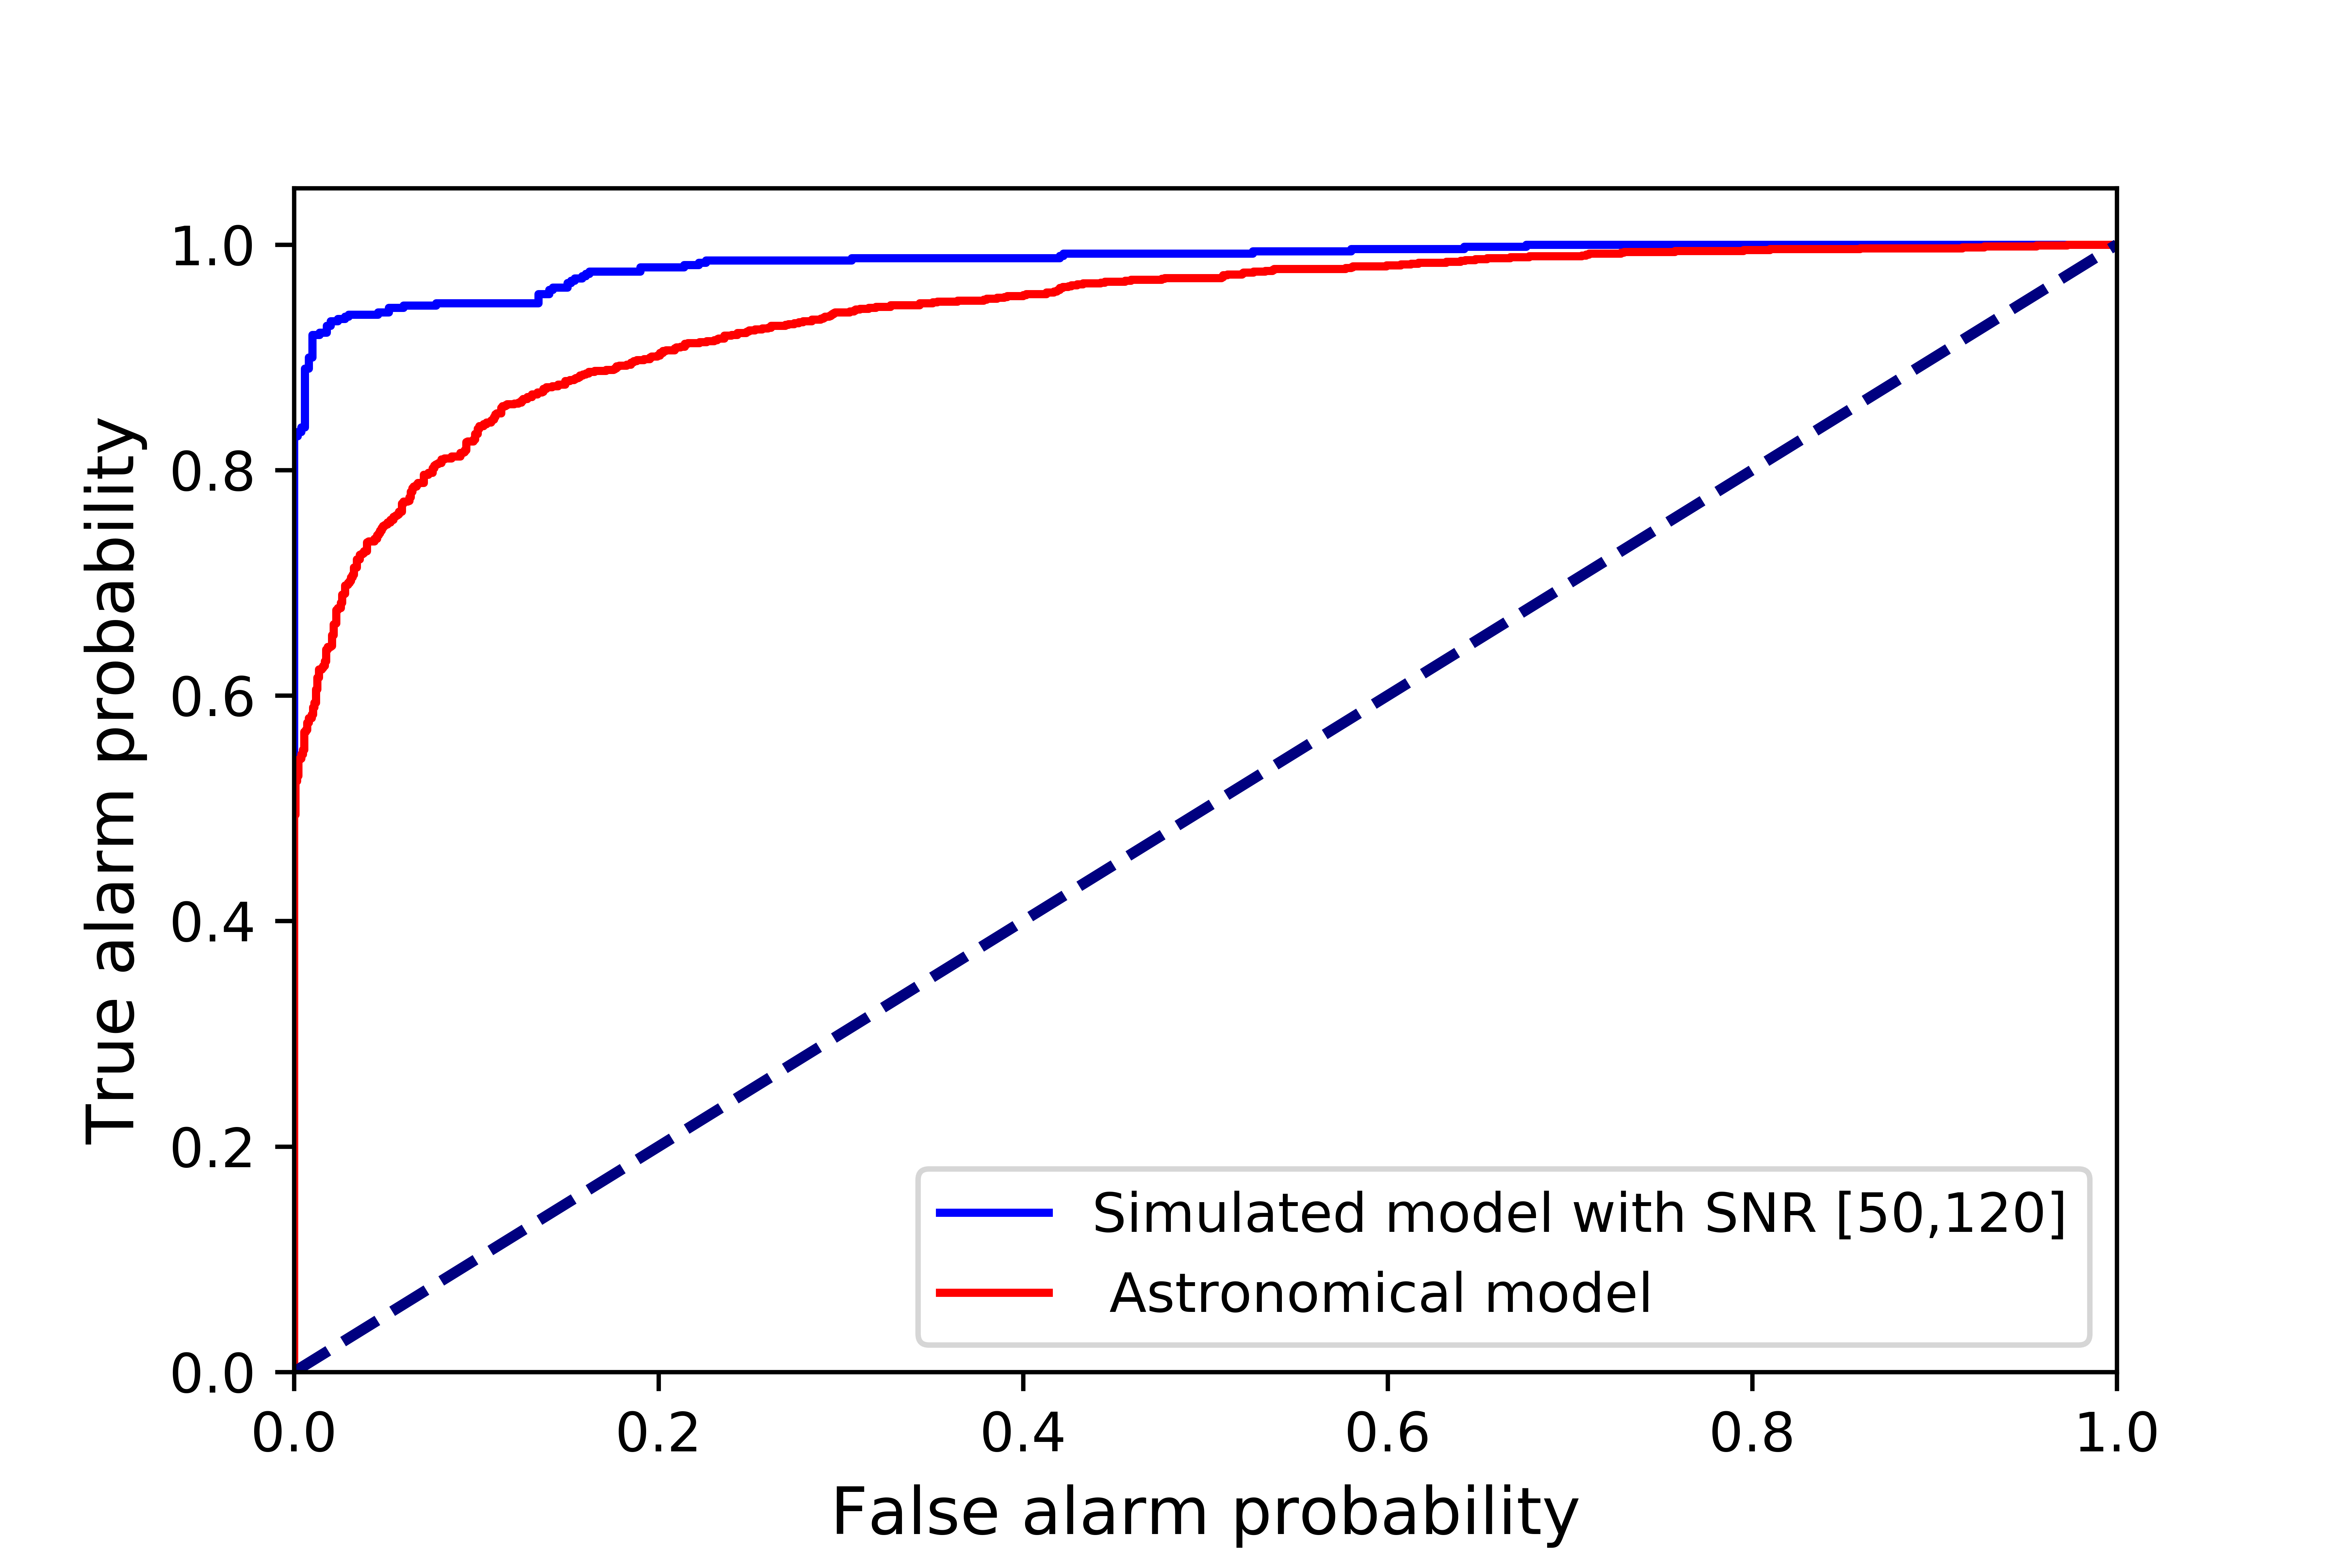
\includegraphics[width=.8\linewidth]{0113-M12-ROCcurve.png}
    \caption{\label{fig:ROC-astro}采用天文学模型模拟得到的EMRI信号测试得到的ROC曲线}
\end{figure}


基于AAK波形,与训练数据独立同分布产生波源参模拟得到EMRI信号的测试数据,即模拟信号的产生除了更换波形模型,源参数的选取跟训练过程中的模拟信号采用同样分布。则分类器得到的ROC曲线如图中\ref{fig:ROC-AAK-iid}红线所示。相比于蓝线,红线与蓝线取得基本一致的结果。这表明采用AK波形和AAK波形所模拟的EMRI信号他们具备了基本一致的EMRI信号特征,这跟原本波形模型的特点是一致的。AAK波形模型就是在参考时间上对相位进行了校准(时间维度的相位偏移),但是保持了AK波形对EMRI信号所建模的相位特点。故而他们能取得一致结果也是可以验证的。
\begin{figure}[!htbp]
 \centering
 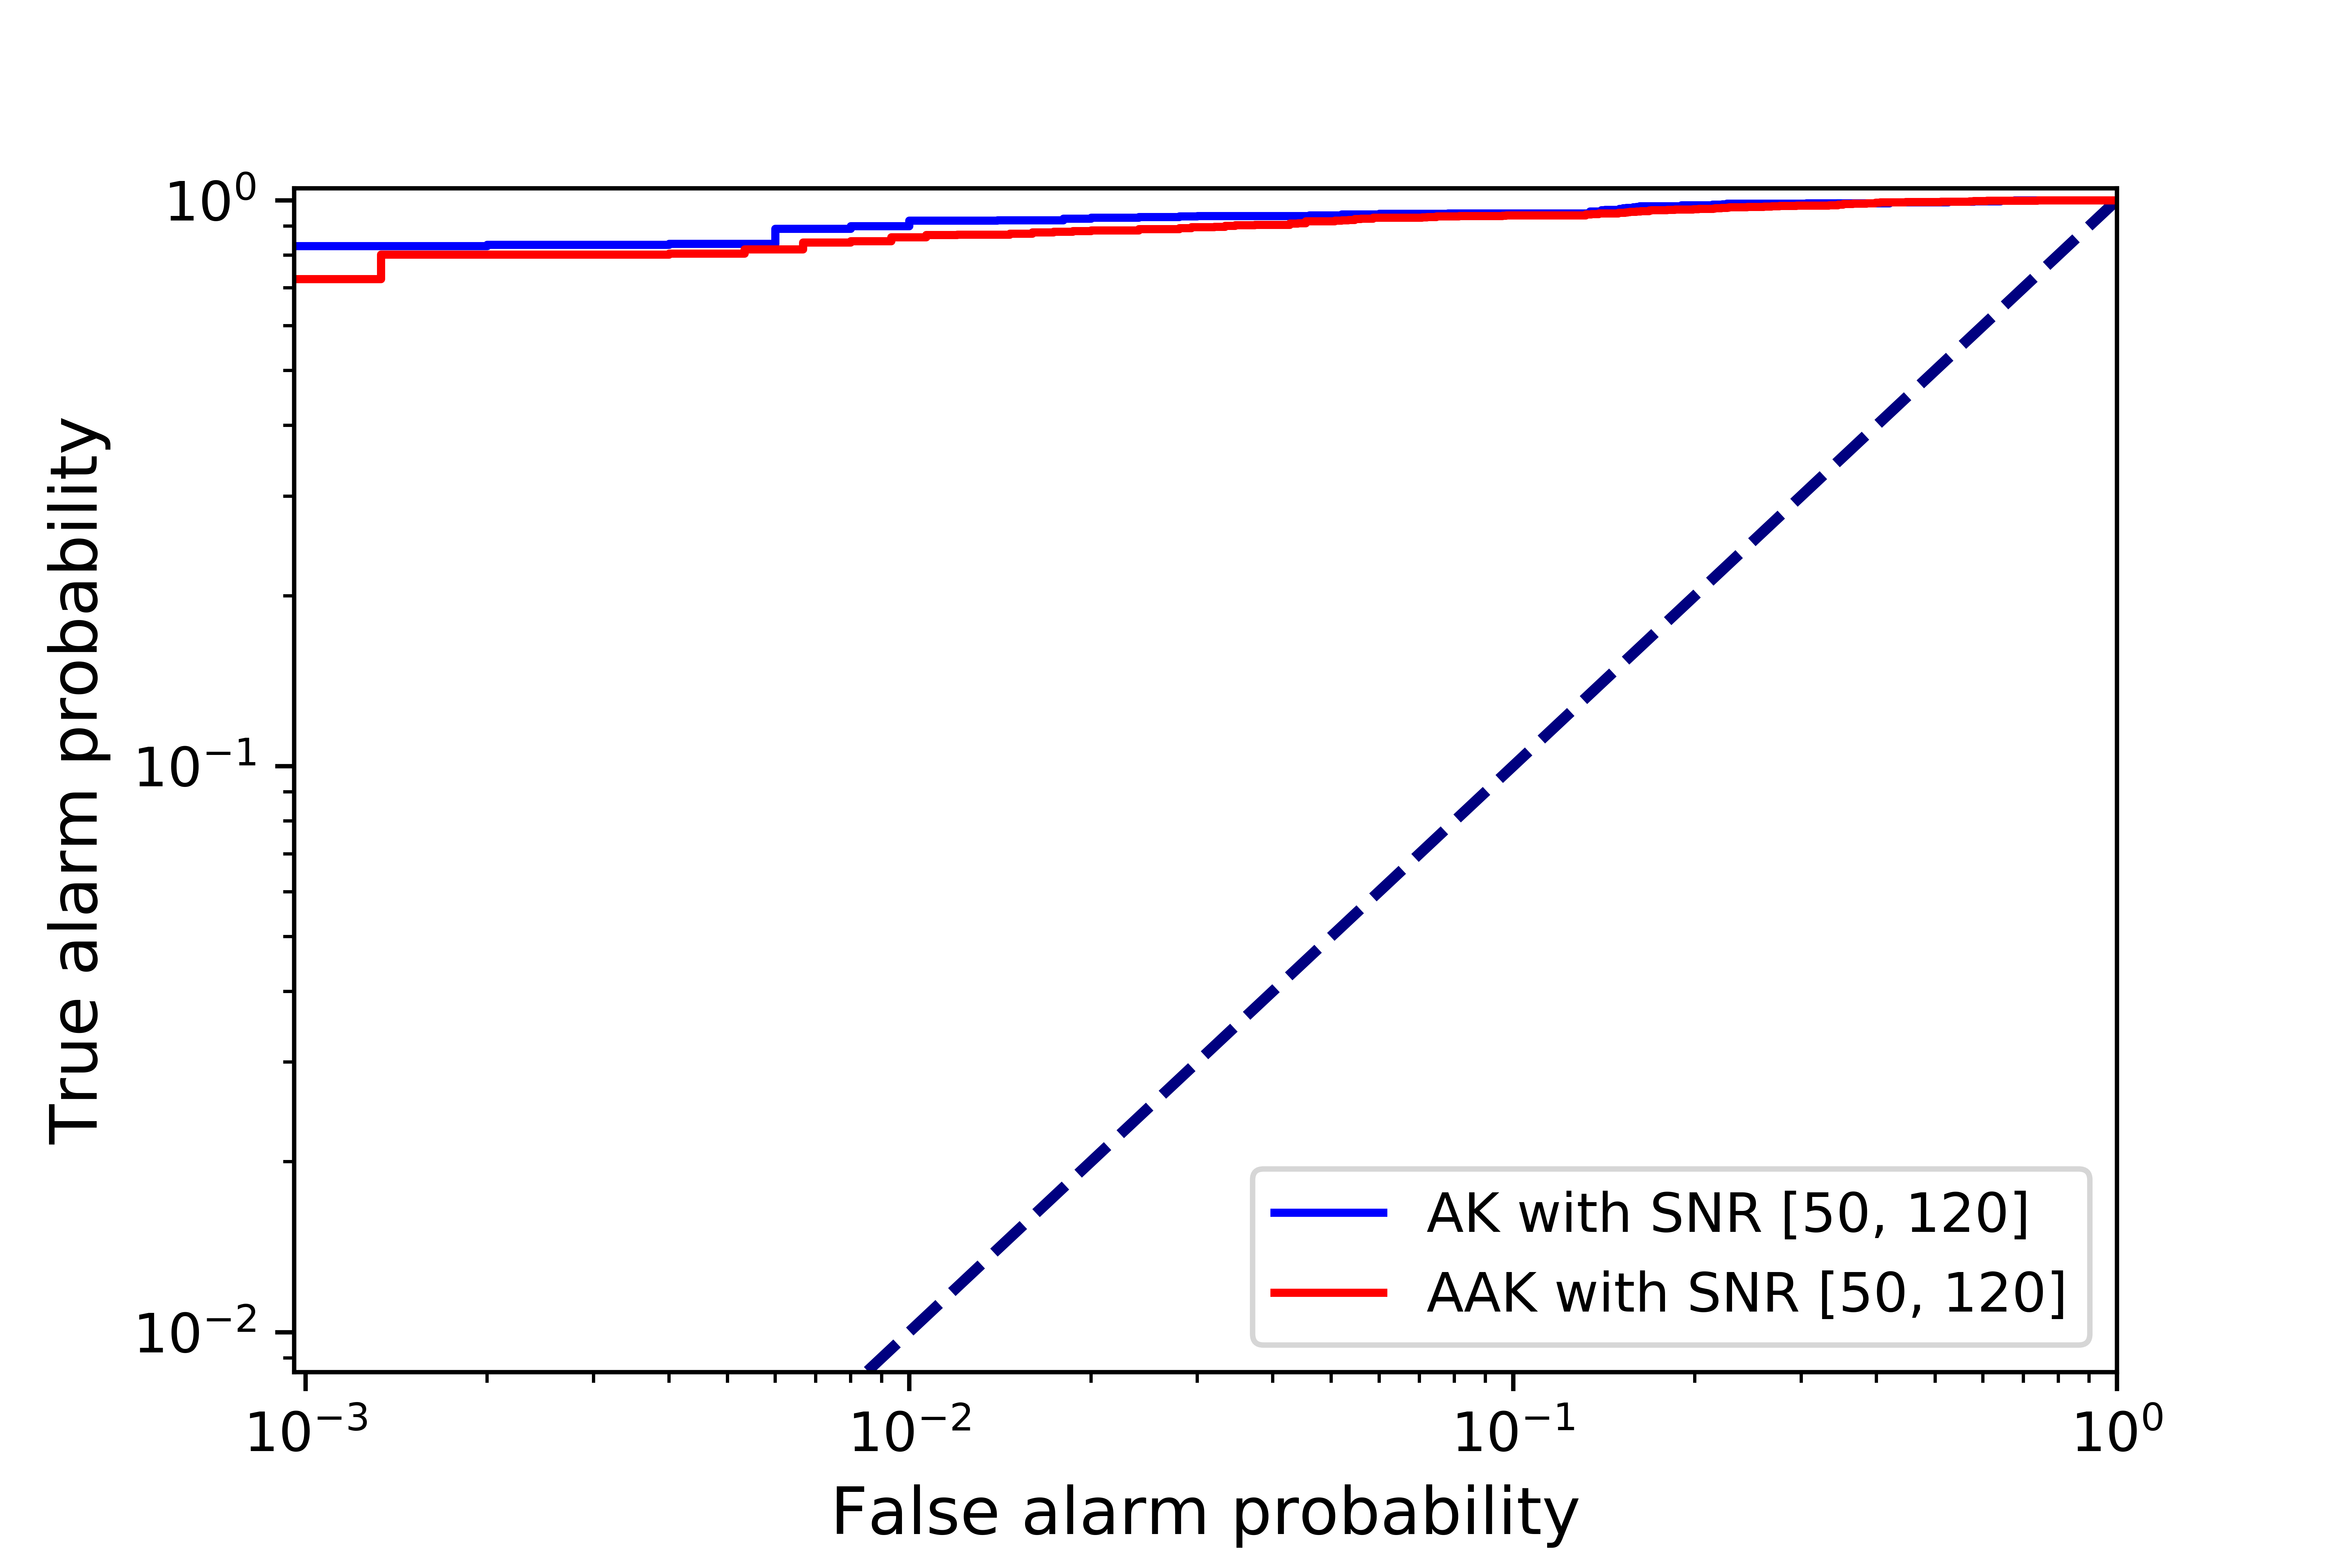
\includegraphics[width=.8\linewidth]{0113-ROC-AAK-AK.png}
\caption{\label{fig:ROC-AAK-iid}基于AAK波形模拟的EMRI信号测试得到的ROC曲线}
\end{figure}

\subsection{有效性曲线}
基于ROC曲线的定义,取固定误报率的前提下,基于AK 模拟的EMRI波形,用以查看对CNN模型对不同源参数的灵敏度变化。在本文中,构造了信号信噪比、中心质量黑洞质量、自旋参数不同的测试数据集,用以测试CNN 模型得到的真正率变化,即类型4-6的测试数据集\ref{tab:test-wave}。

第一,构造了固定信噪比不同的EMRI波形,比如构造了信噪比为10的EMRI信号和信噪比为130的EMRI信号,各2000个。把这两个数据集都用该分类器进行测试性能,分别设置误报率为1\%和0.1\%时,得到两个真正率(TPR)。同理可以构造其他固定信噪比的数据集,得到相应的真正率,绘制有效性曲线,结果如图\ref{fig:EC-SNR}所示。
\begin{figure}[!htbp]
\centering
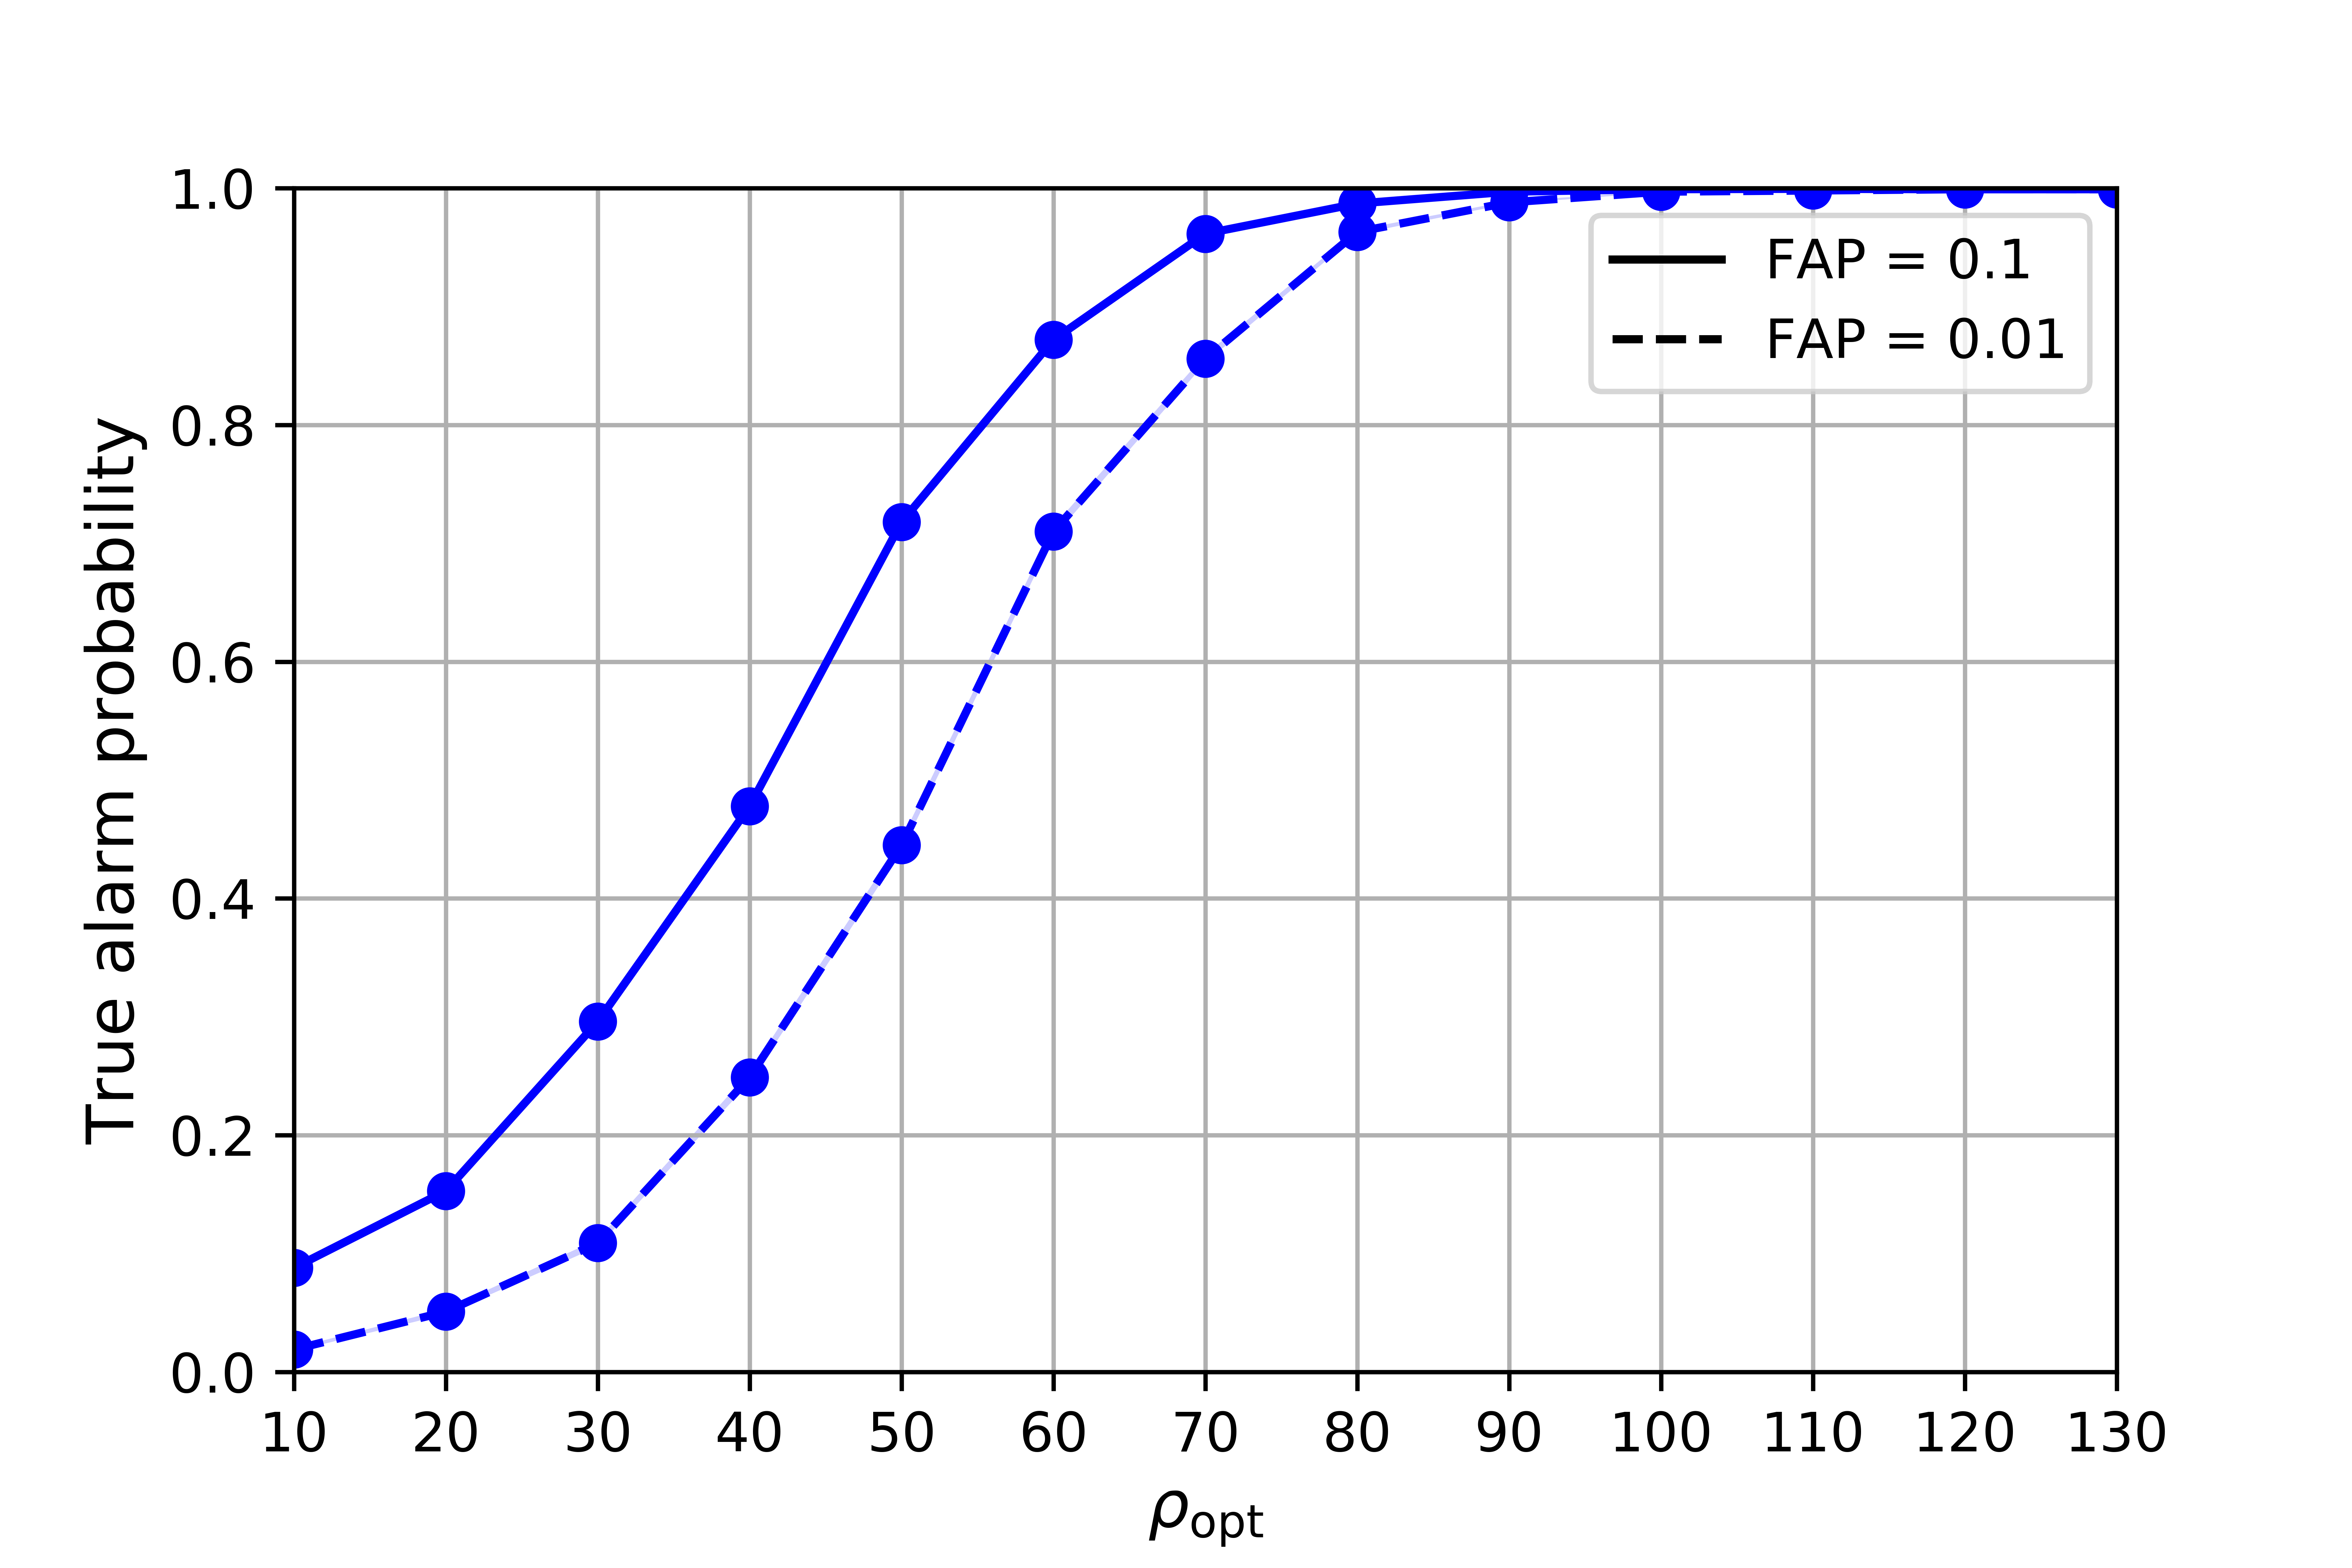
\includegraphics[width=.8\linewidth]{efficiency-SNR.png}
\caption{\label{fig:EC-SNR}有效性曲线:含有固定信噪比不同模拟信号的测试数据集}
\end{figure}

第二,构造了不同固定中心黑洞质量的EMRI波形的数据集。其中自旋固定为0.98,其他源参数随机产生。每个测试数据集数目为2000个,其中1000个模拟信号,1000 个模拟噪声。得到的真正率随中心黑洞质量该参数变化的曲线,结果如图\ref{fig:EC-SMBHmass}所示。
\begin{figure}[!htbp]
 \centering
 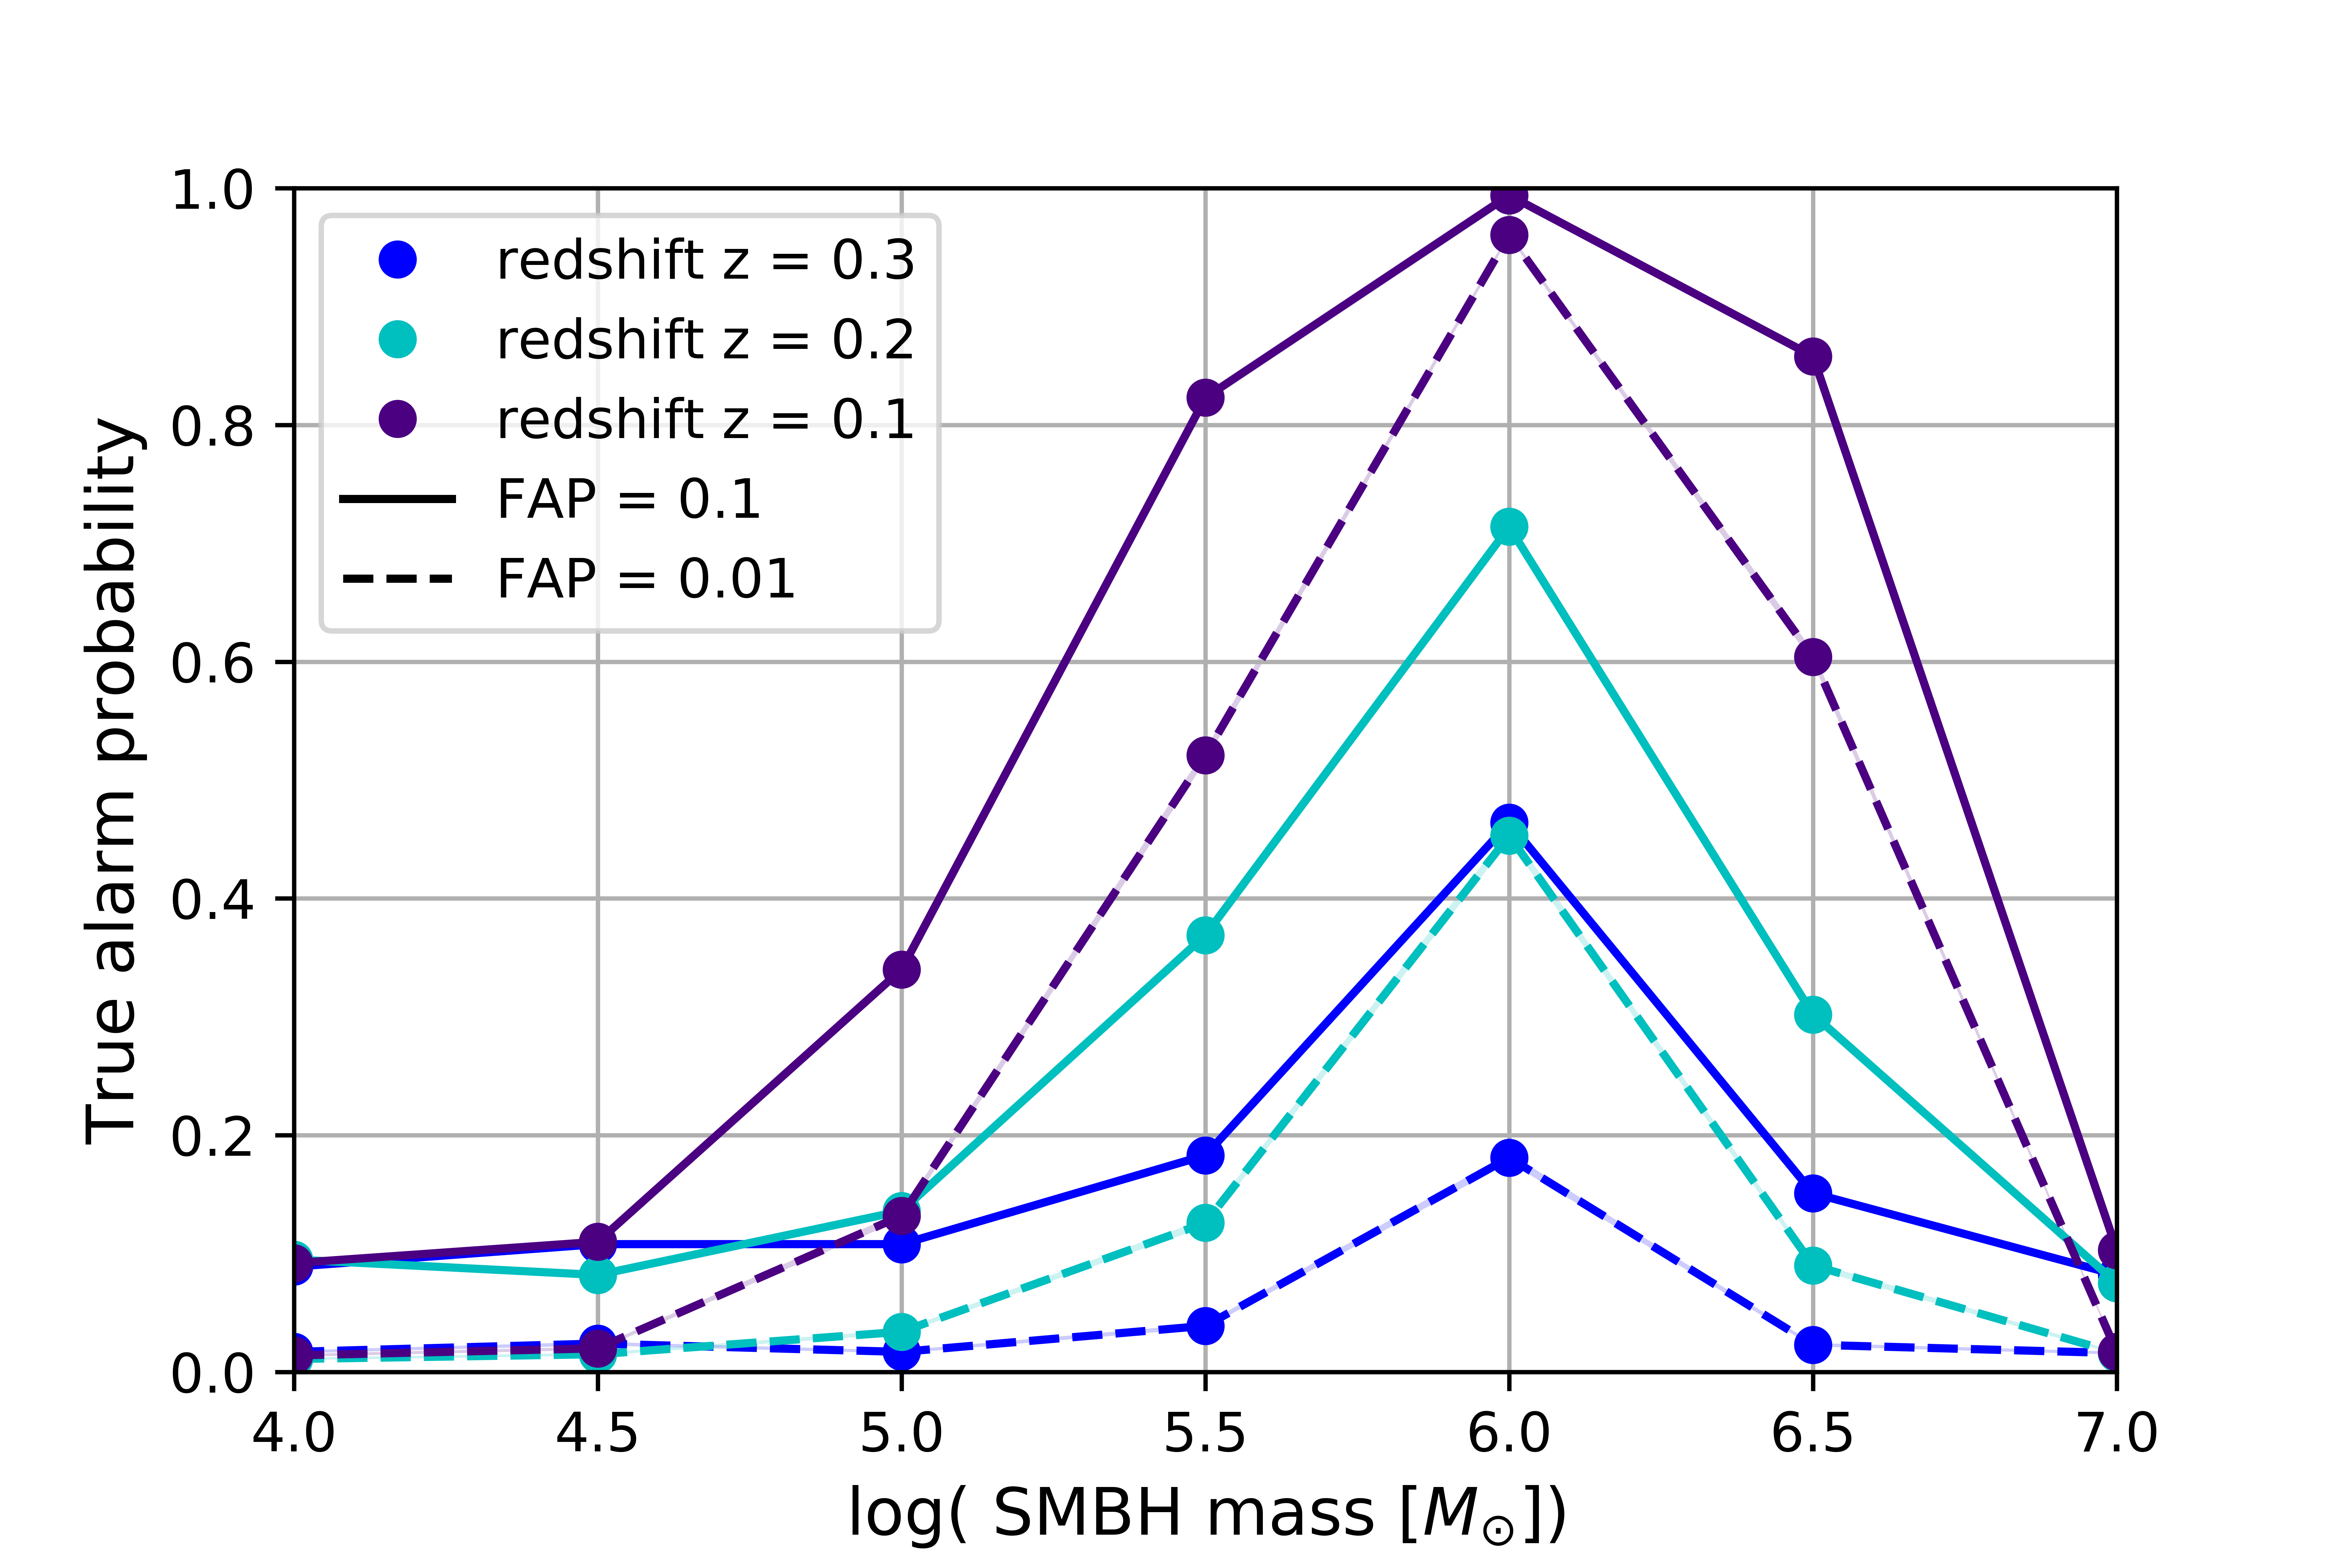
\includegraphics[width=.8\linewidth]{efficiency-SMBHmass.png}
    \caption{\label{fig:EC-SMBHmass}有效性曲线:含有固定中心大质量黑洞不同模拟信号的测试数据集}
\end{figure}

第三,构造了不同中心黑洞自旋的EMRI波形的数据集。设置中心大质量黑洞为$10^6 M_{\odot}$,其他源参数随机产生,不调整信噪比。同理,每个测试数据集数目也为2000个,模拟信号和模拟噪声各占一半。则得到的真正率随中心黑洞自旋该参数变化的曲线,结果如图\ref{fig:EC-Spin}所示。
\begin{figure}[!htbp]
 \centering
 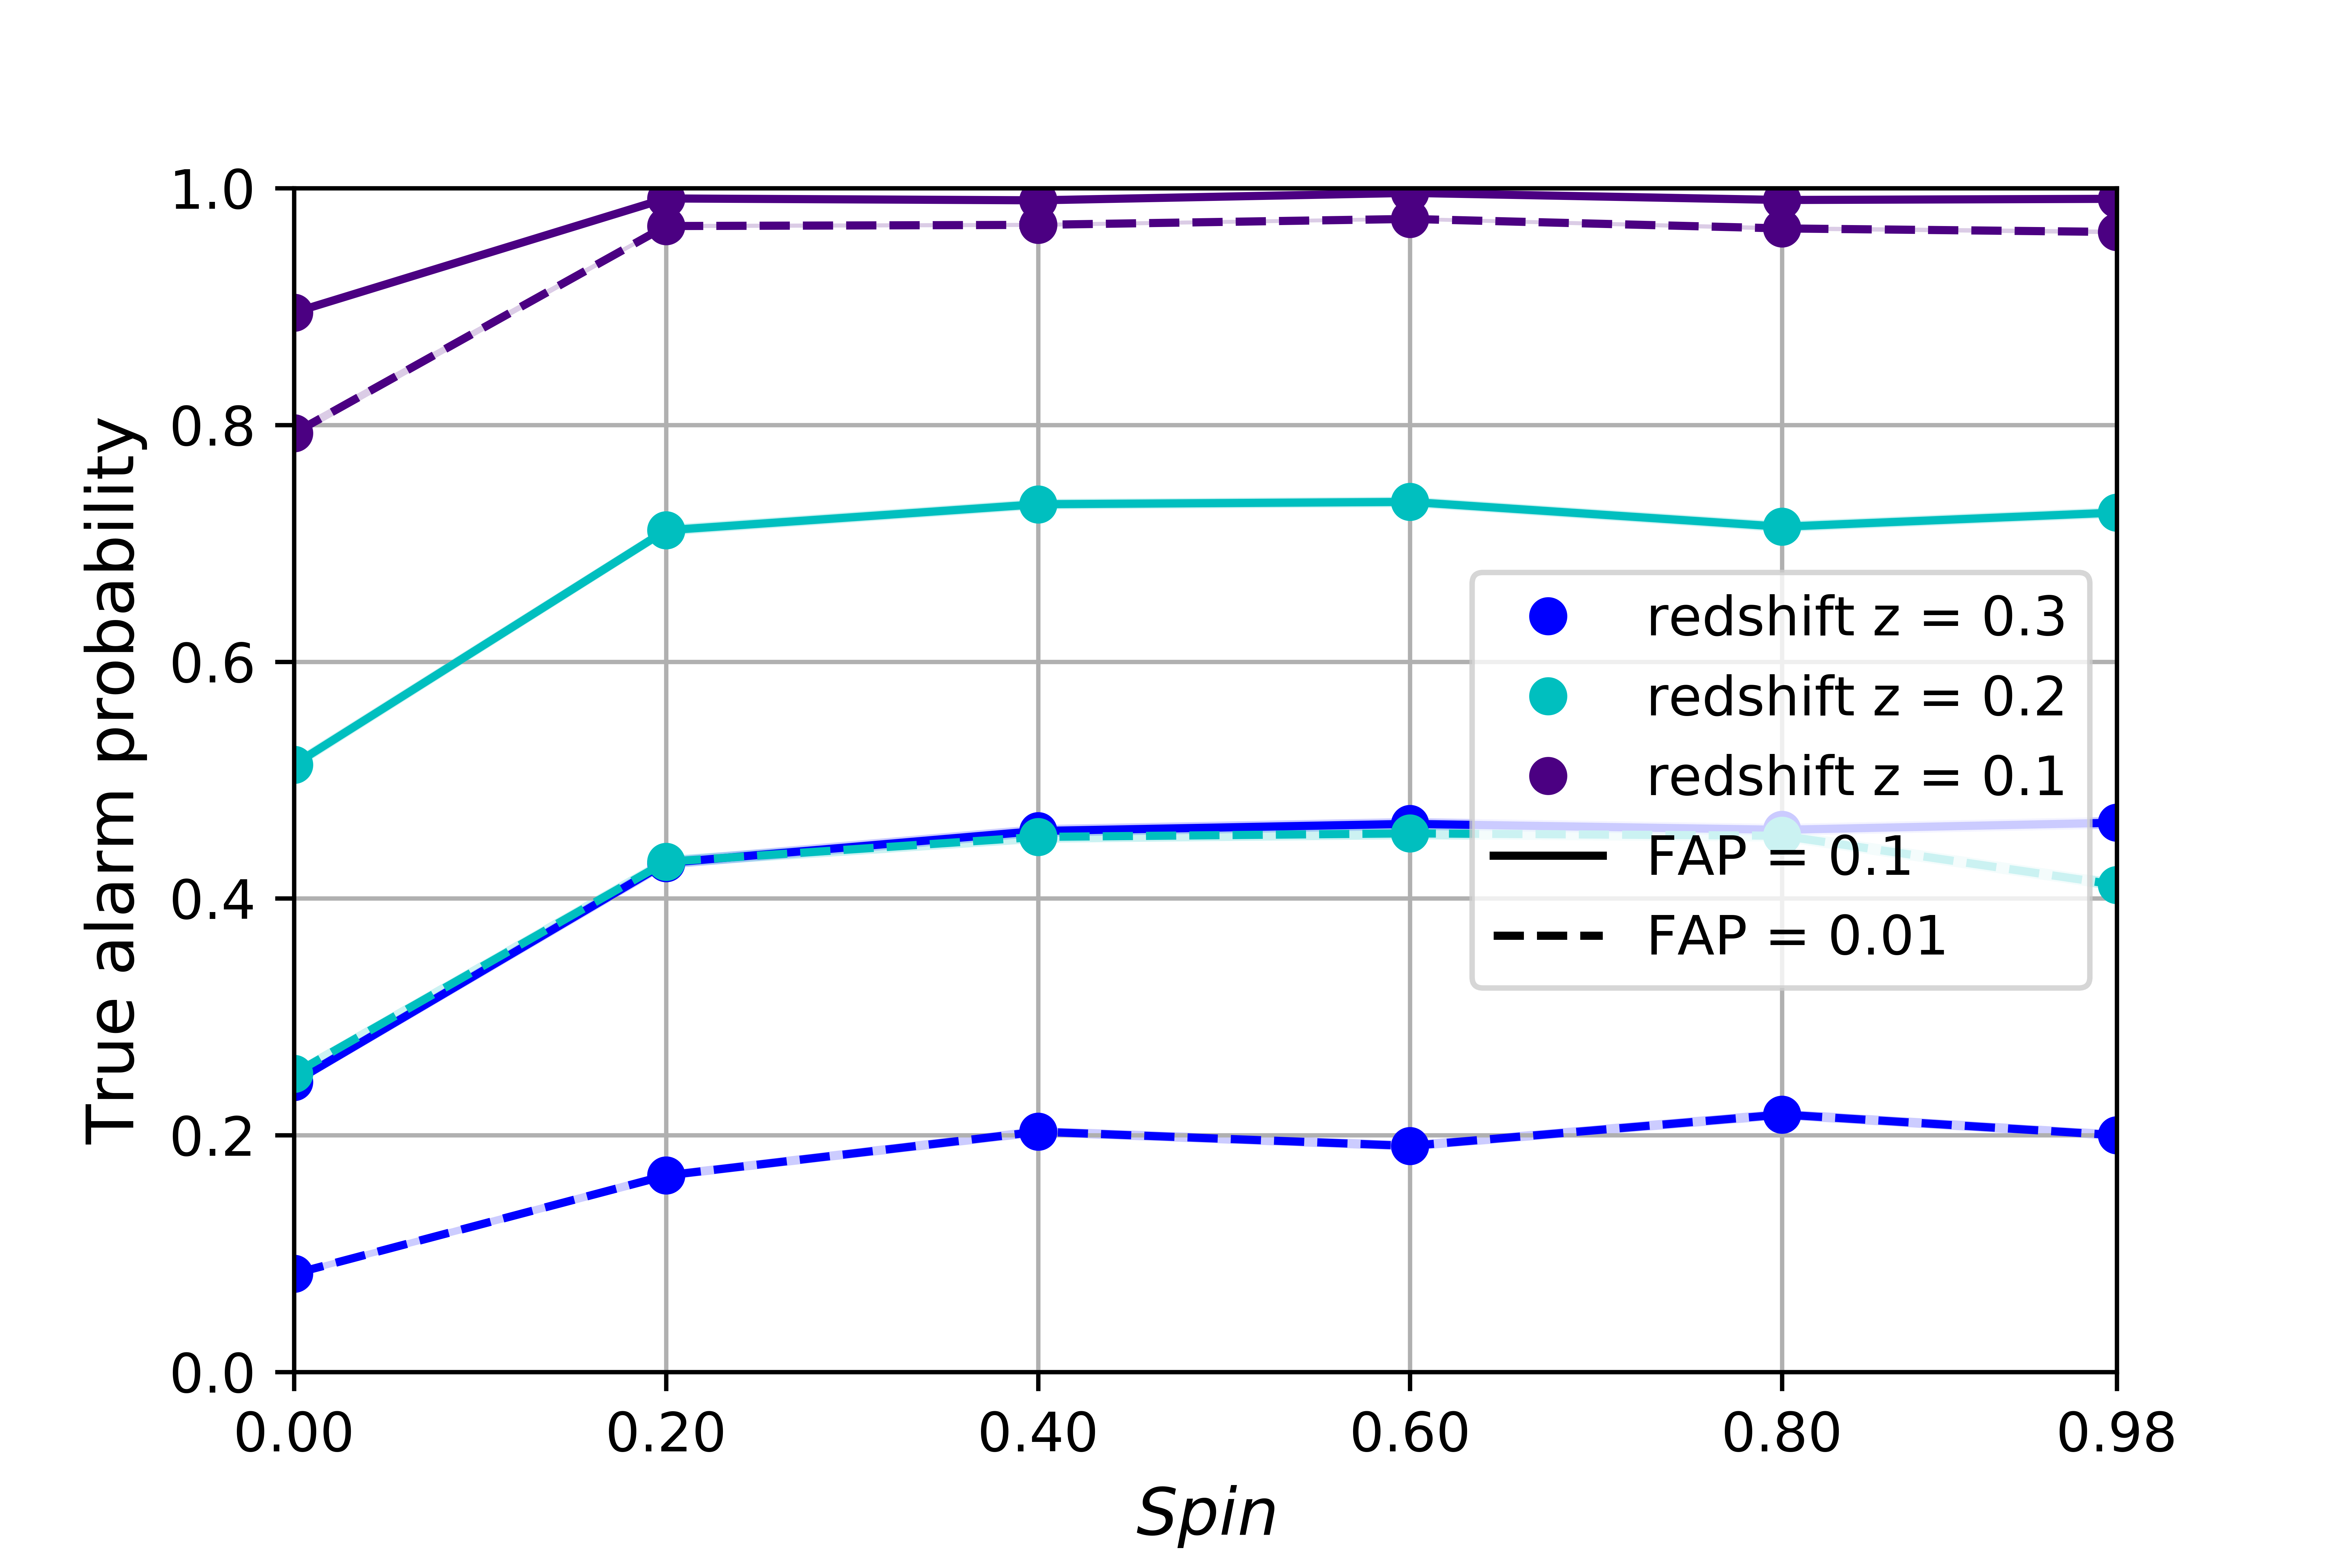
\includegraphics[width=.8\linewidth]{efficiency-Spin.png}
    \caption{\label{fig:EC-Spin}有效性曲线:含有固定大质量黑洞自旋不同模拟信号的测试数据集}
\end{figure}

\begin{figure}[!htbp]
\centering
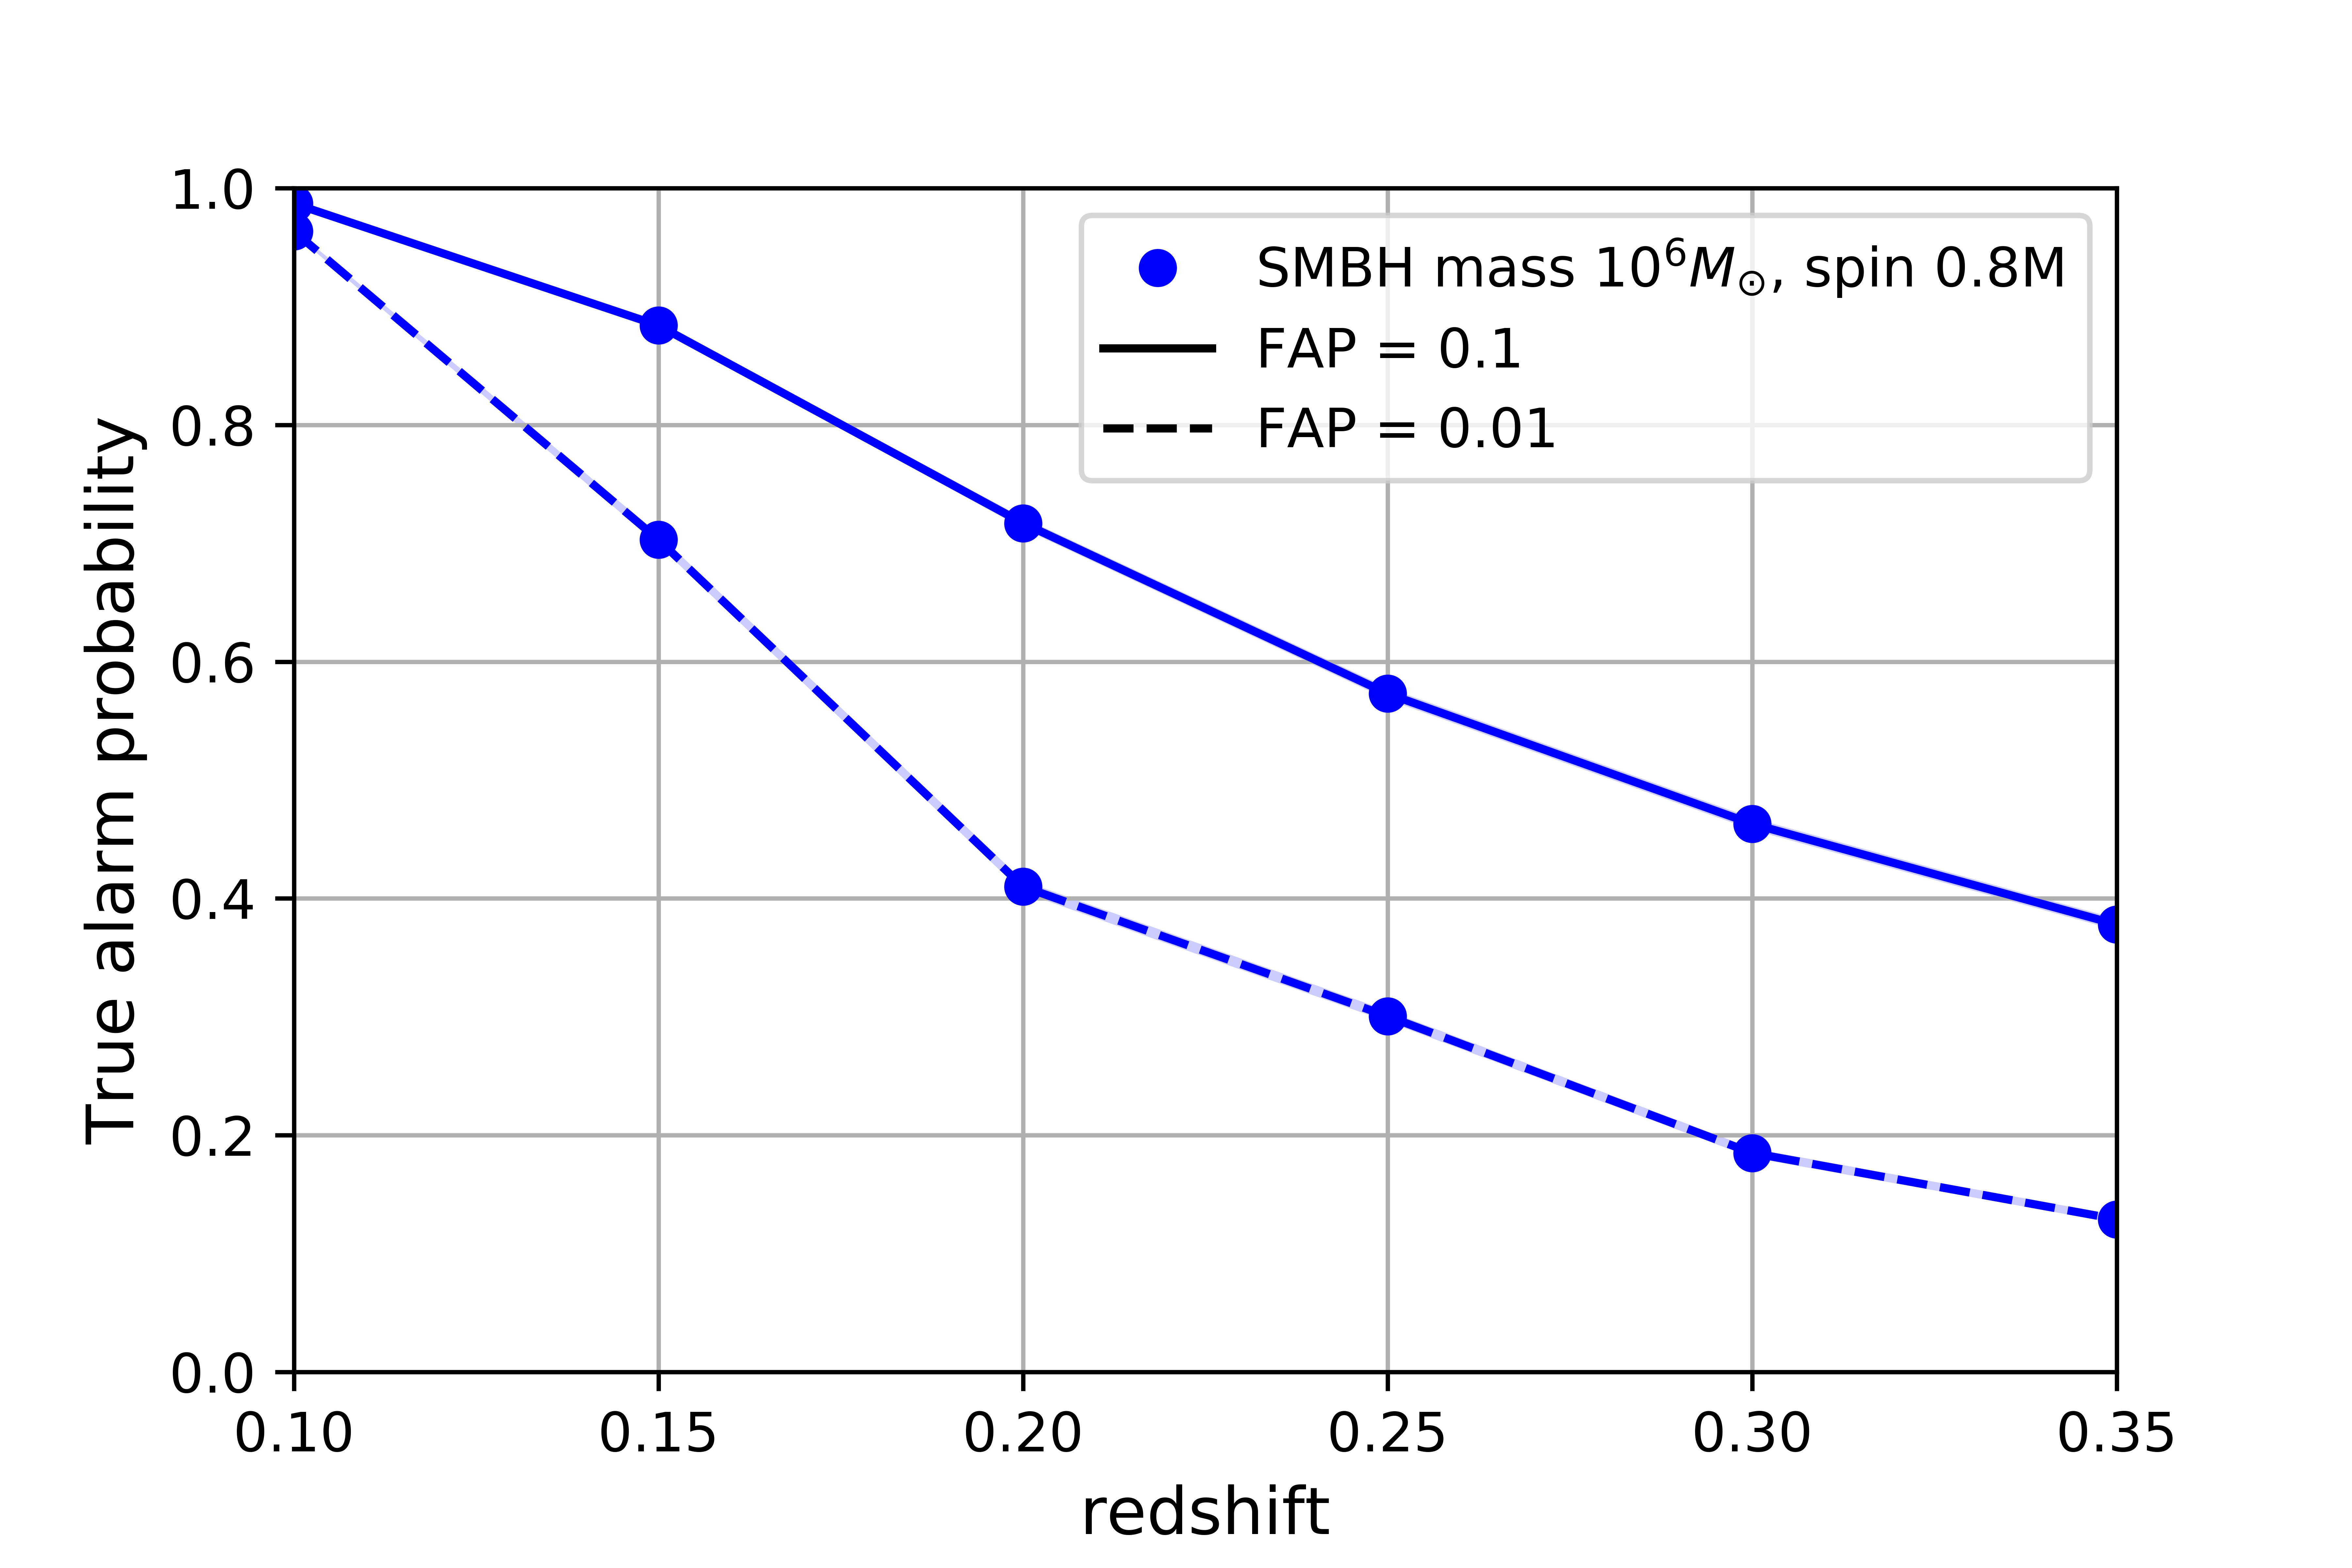
\includegraphics[width=.8\linewidth]{efficiency-Redshift.png}
\caption{\label{fig:EC-SNR}有效性曲线:含有固定信噪比不同模拟信号的测试数据集}
\end{figure}


%\chapter{EMRI信号参数估计}
%现有参数估计的方法及结果

%\chapter{数据处理流水线设计:以EMRI波源数据处理提出需求}
% !Mode:: "TeX:UTF-8"

\chapter{总结及展望}

结束语:画龙点睛

归纳全文的创新点

指出下一步需要开展的工作

约3页左右,3000字左右

%总结



%%====================
%% 参考文献

%\addcontentsline{toc}{chapter}{\bibname}
\bibliographystyle{gbt7714-2005}
\bibliography{refs}

\clearpage

\backmatter

%%====================
%% 发表工作
% !Mode:: "TeX:UTF-8"

\markboth{攻读硕士学位期间发表学术论文情况}{攻读硕士学位期间发表学术论文情况}
\addcontentsline{toc}{chapter}{攻读硕士学位期间发表学术论文情况}
%\setcounter{page}{1}       % 如果需要从该页开始从 1 开始编页,则取消该注释
\chapter*{攻读硕士学位期间发表学术论文情况}

%\noindent[1] \textbf{Bao, J.}, Shi, C., Wang, H., Zhang, J. D., Hu, Y. M., Mei, J., and Luo, J. (2019). Constraining modified gravity with ringdown signals: An explicit example. Physical Review D, 100(8), 084024.

\clearpage
\mainmatter

% !Mode:: "TeX:UTF-8"

\markboth{致\quad 谢}{致\quad 谢}
\addcontentsline{toc}{chapter}{致\quad 谢} % 添加到目录中
\chapter*{致\quad 谢}
几年的研究生生活过去很快,

感谢老师

感谢领导

感谢同学

感谢父母

感天动地


\end{document}
